\section{A Toy Model}
%
%
\begin{frame}
  So far we have worked out a sound theoretical foundation to understand the
  errors incurred when building learning algorithms.  In this section we will
  analyze in detail how these concepts look with a toy model.
\end{frame}
%
%
\begin{frame}
  Our data generating process will be very simple so that we can fully analyse
  the situation:

  \begin{align*}
    X &\sim U(0, 2 \pi) \\
    Y &\sim \sin(X) + N(0, \epsilon)
  \end{align*}

  Where $U$ is the uniform distribution on an interval, and $N$ is the normal
  distribution with a given mean and variance.
\end{frame}
%
%
\begin{frame}
  \begin{figure}
    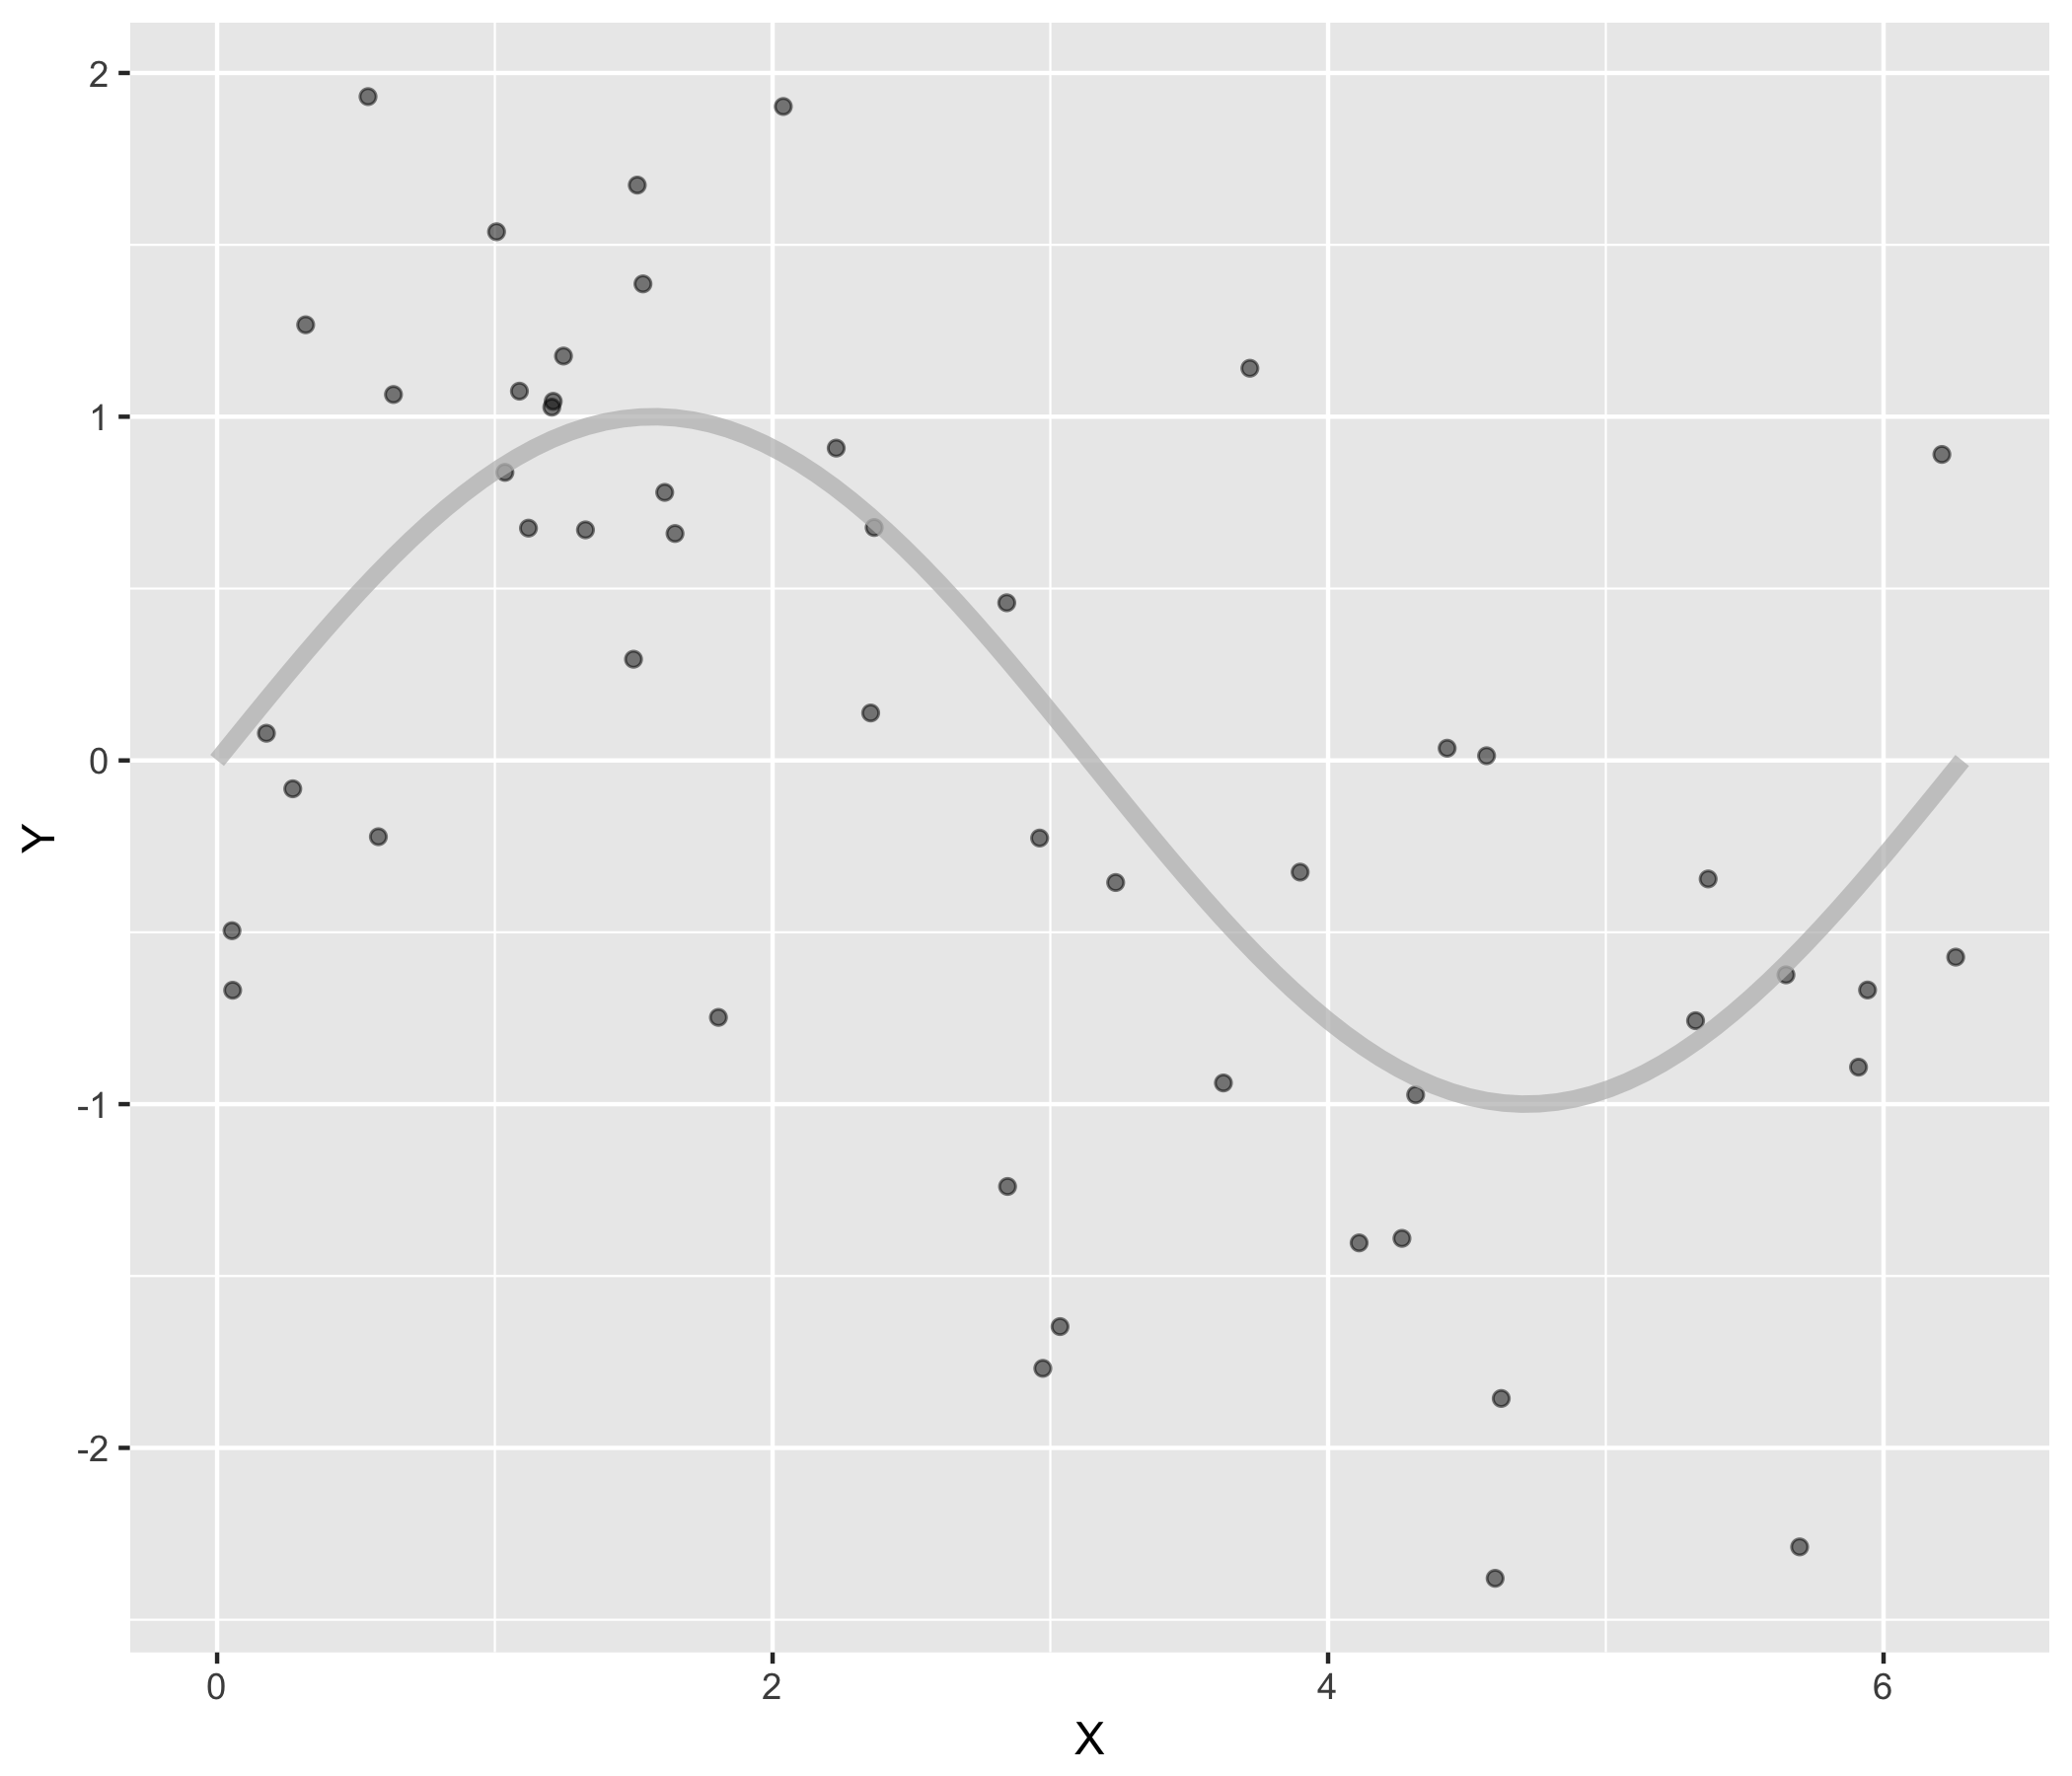
\includegraphics[scale=0.09]{true_signal}
  \end{figure}

  Clearly, the regression function $E(Y \mid X)$ is given by:
  $$ \F(X) = E[ \sin(x) + N(0, \epsilon) \mid x ] = \sin(x) $$
\end{frame}
%
%
\begin{frame}
  The irreducible error component, which does not depend on our choice of
  learning algorithm, is easy to compute straight from the definition:

  \begin{align*}
      \IESE(x) &= E_Y \left[ \left( y - \F(x) \right)^2 \mid x \right] \\
      &= E_Y \left[ \left( \sin(x) + N(0, \epsilon) - \sin(x) \right)^2 \right] \\
      &= E_Y \left[ N(0, \epsilon)^2 \right] \\
      &= \epsilon
  \end{align*}
   
\end{frame}
%
%
\begin{frame}
  We take as our learning algorithm \textbf{linear regression}:
  $$ \LinReg: \D \mapsto \LinReg({\D}_{X}, {\D}_{Y}) $$
  \begin{figure}
    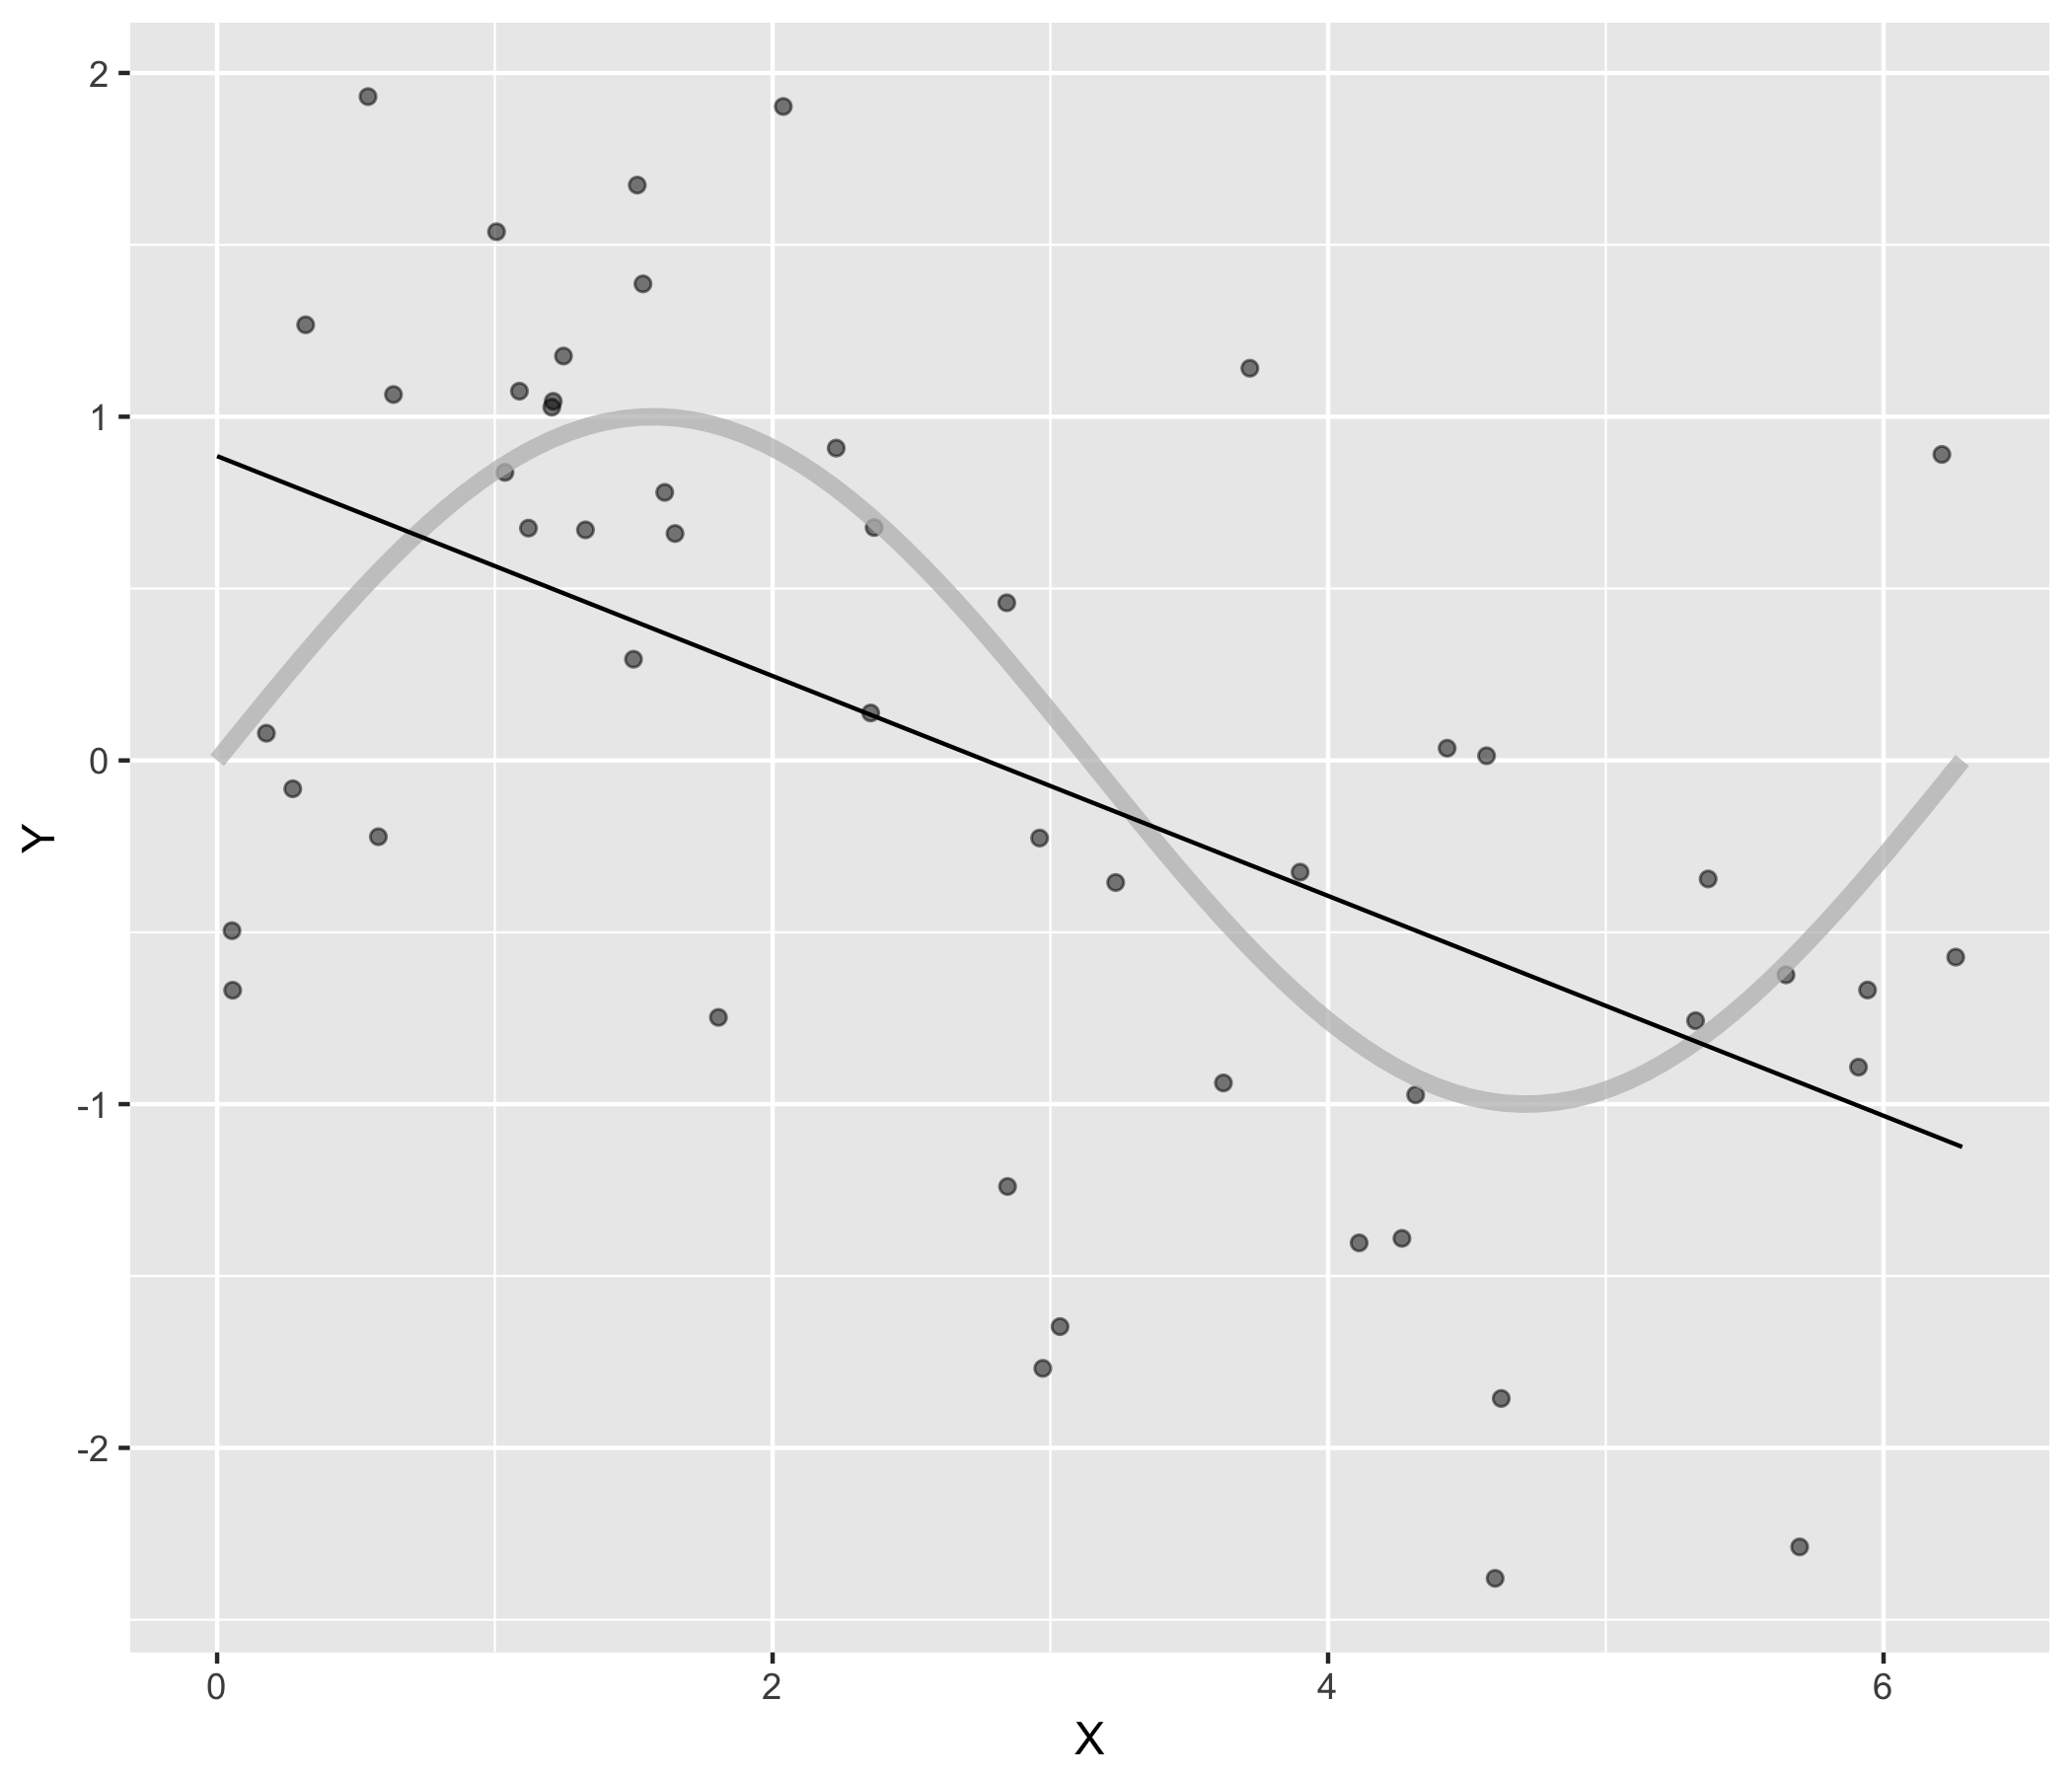
\includegraphics[scale=0.09]{single_fitted_line}
  \end{figure}
\end{frame}
%
%
\begin{frame}
  Let's study the bias of our toy model.  Recall the definition:
  \begin{align*}
    \BIAS (x)^2 = \left( \F(x) - Ef(x) \right)^2
  \end{align*}
  Where:
  \begin{align*}
    Ef(x) = E_D \left[ f(x; \D) \mid x \right] \\ 
  \end{align*}
  is the expected output of our modeling algorithm.
\end{frame}
%
%
\begin{frame}
  For our toy situation we can calculate $Ef$ numerically (I used scipy):
  $$ Ef(x) \approx -0.304 x +  0.955 $$
\end{frame}
%
%
\begin{frame}
  \begin{figure}
    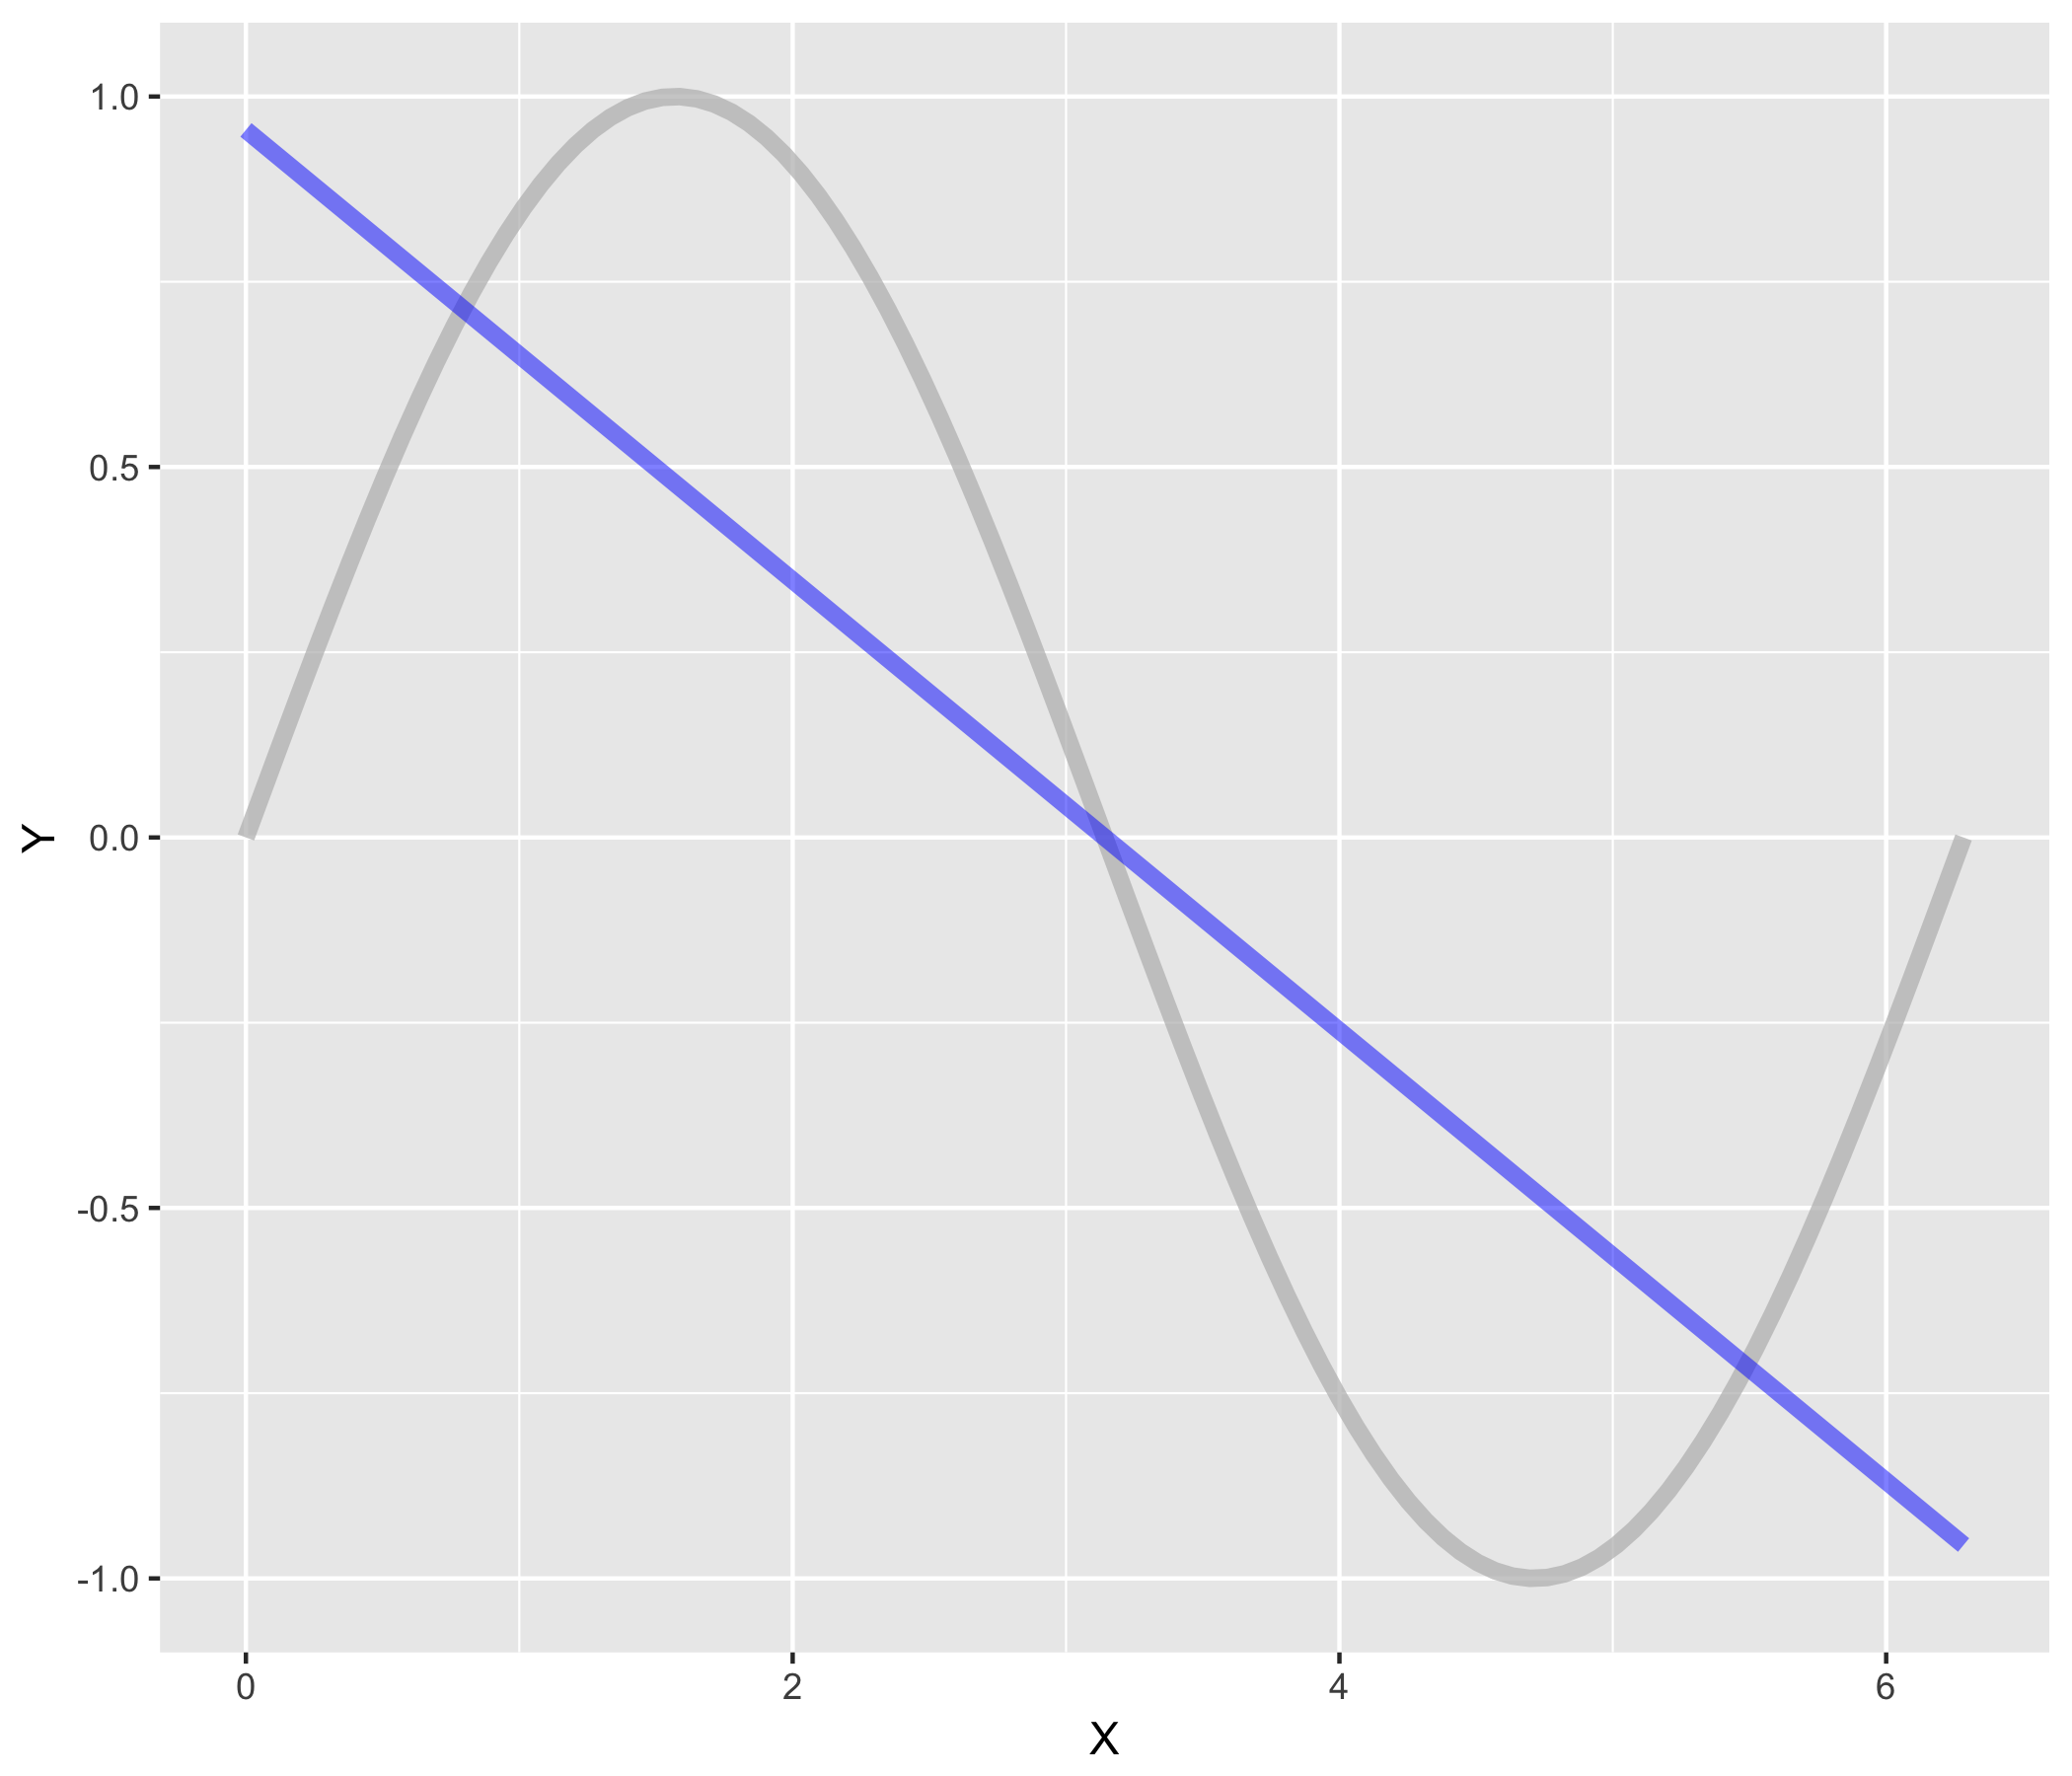
\includegraphics[scale=0.12]{best_linear_fit}
  \end{figure}
\end{frame}
%
%
\begin{frame}
  The bias at a point is the square of the vertical distance between the true
  signal and the best linear fit.
  \begin{figure}
    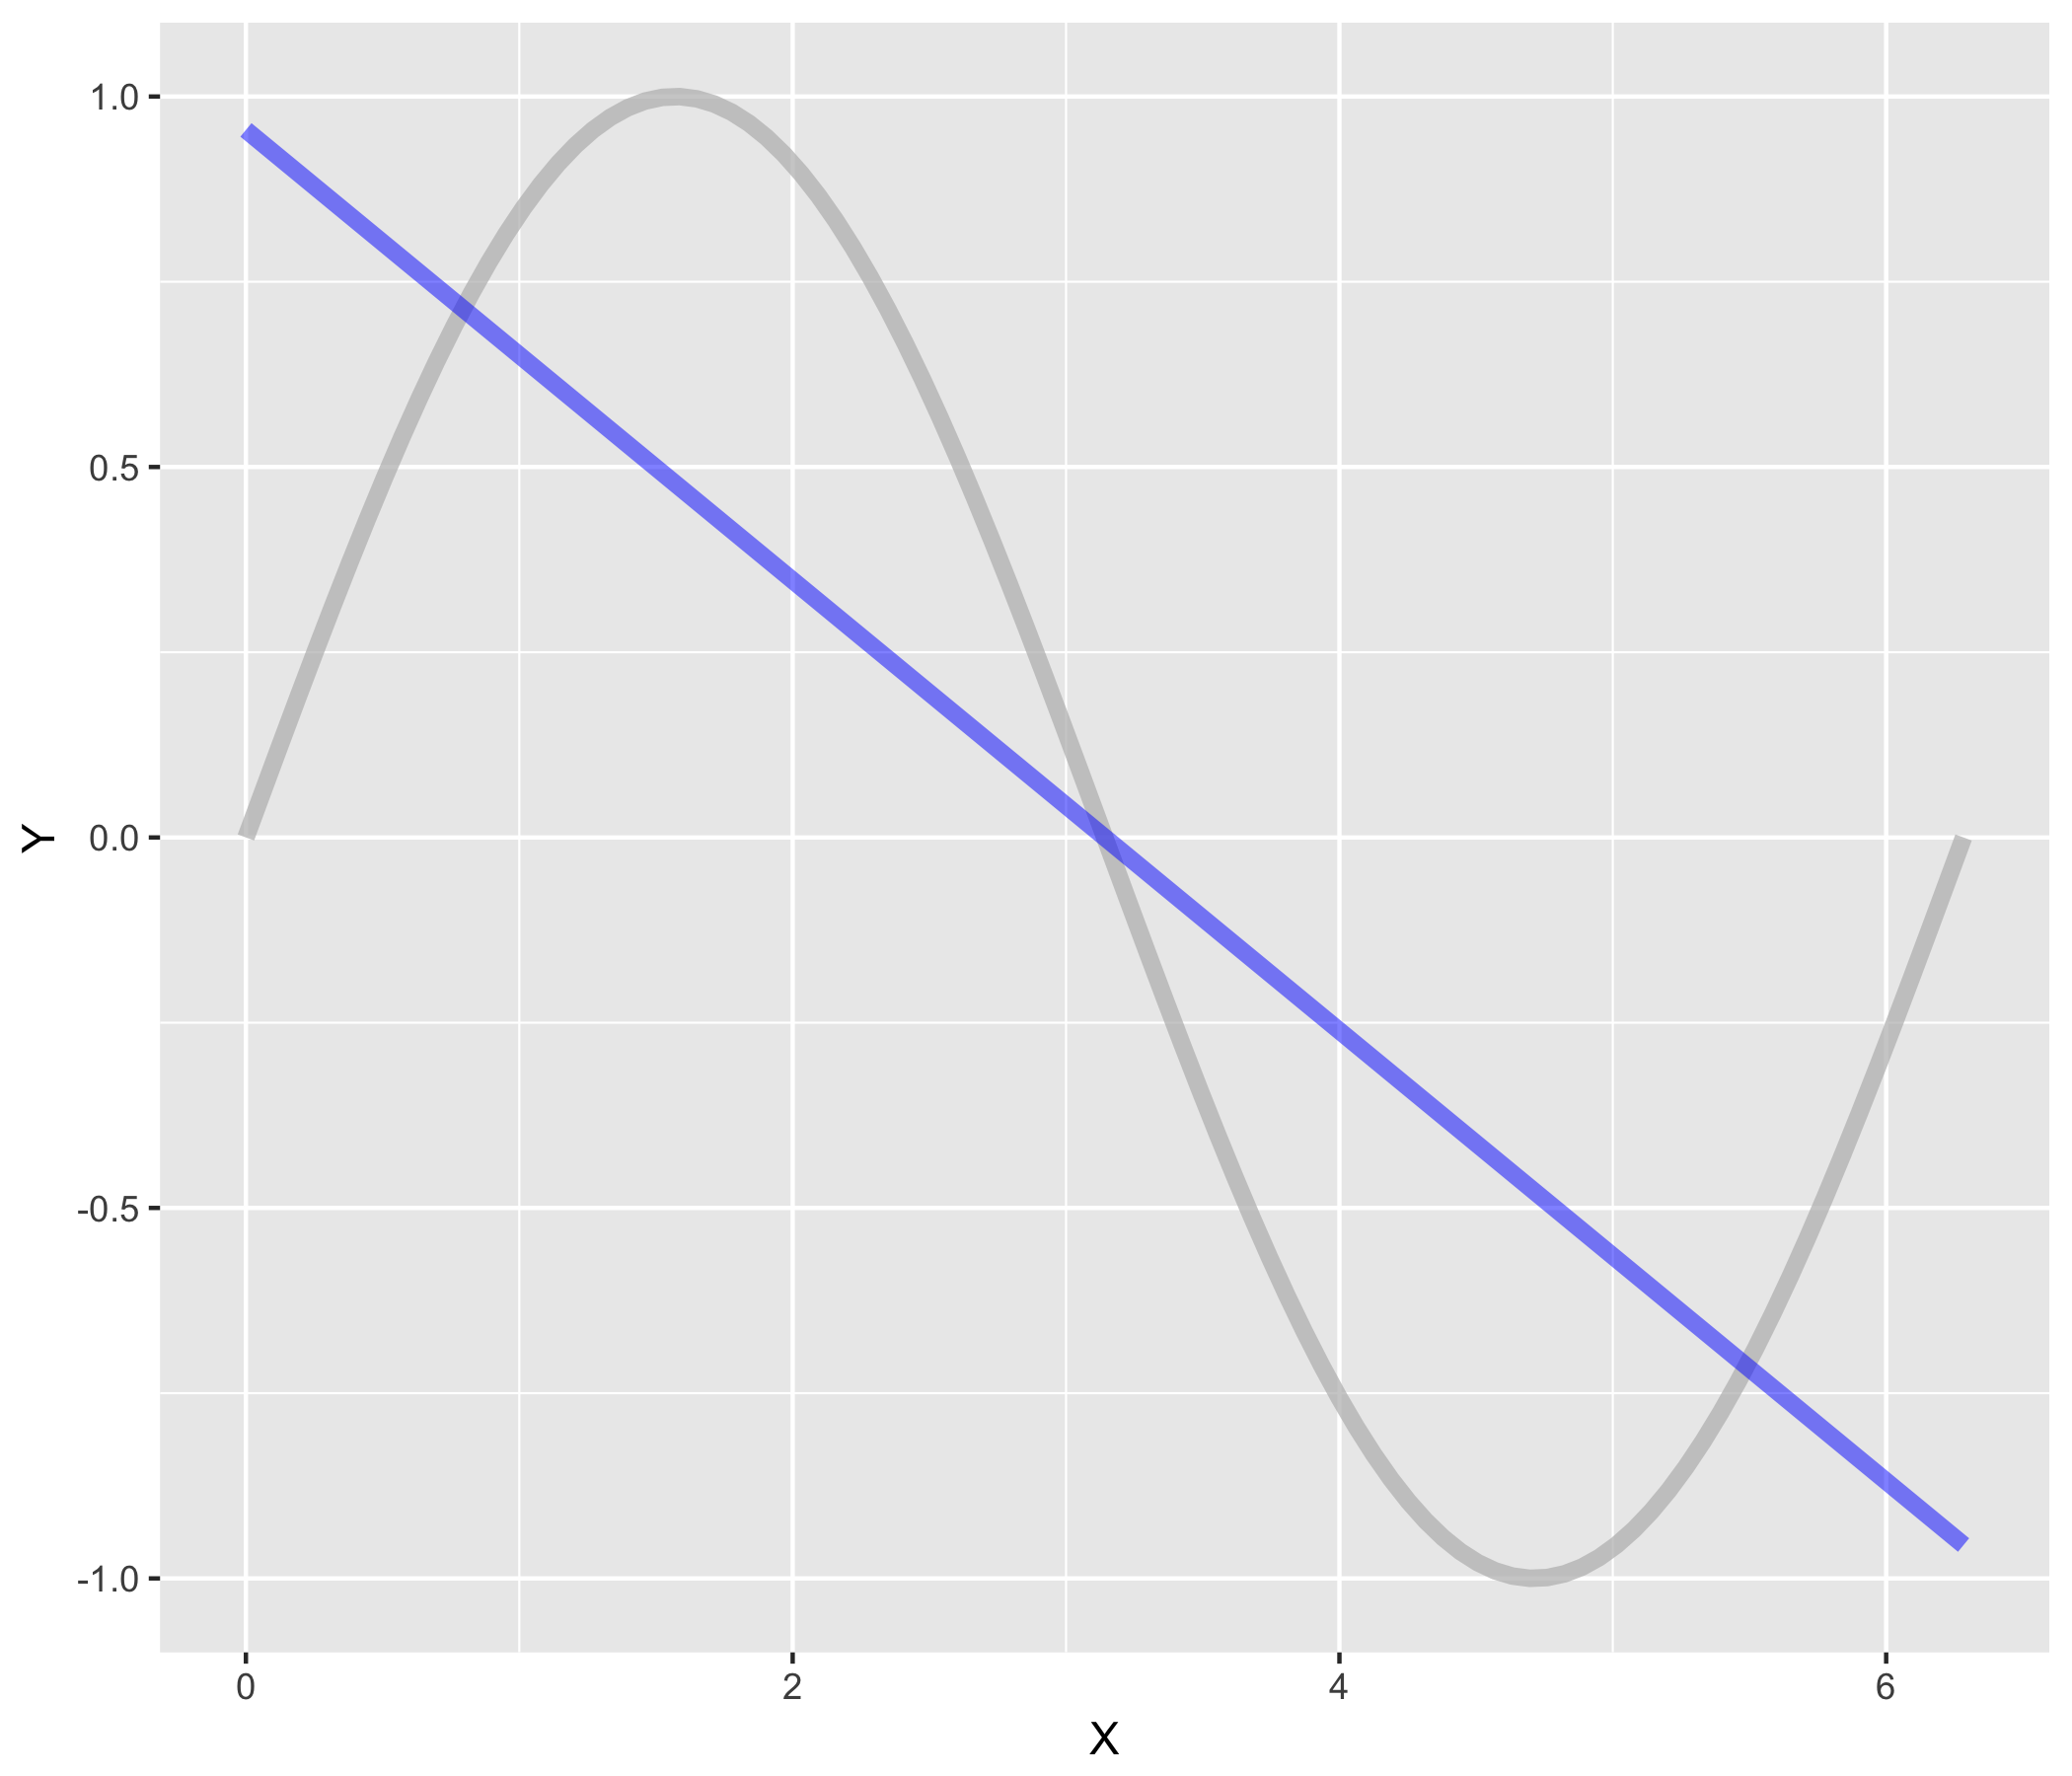
\includegraphics[scale=0.08]{best_linear_fit}
  \end{figure}
\end{frame}
%
%
\begin{frame}
  The total bias is the expectation of the pointwise bias.  Visually, we can
  think of the unsigned area between the best linear fit and the true signal:
  \begin{figure}
    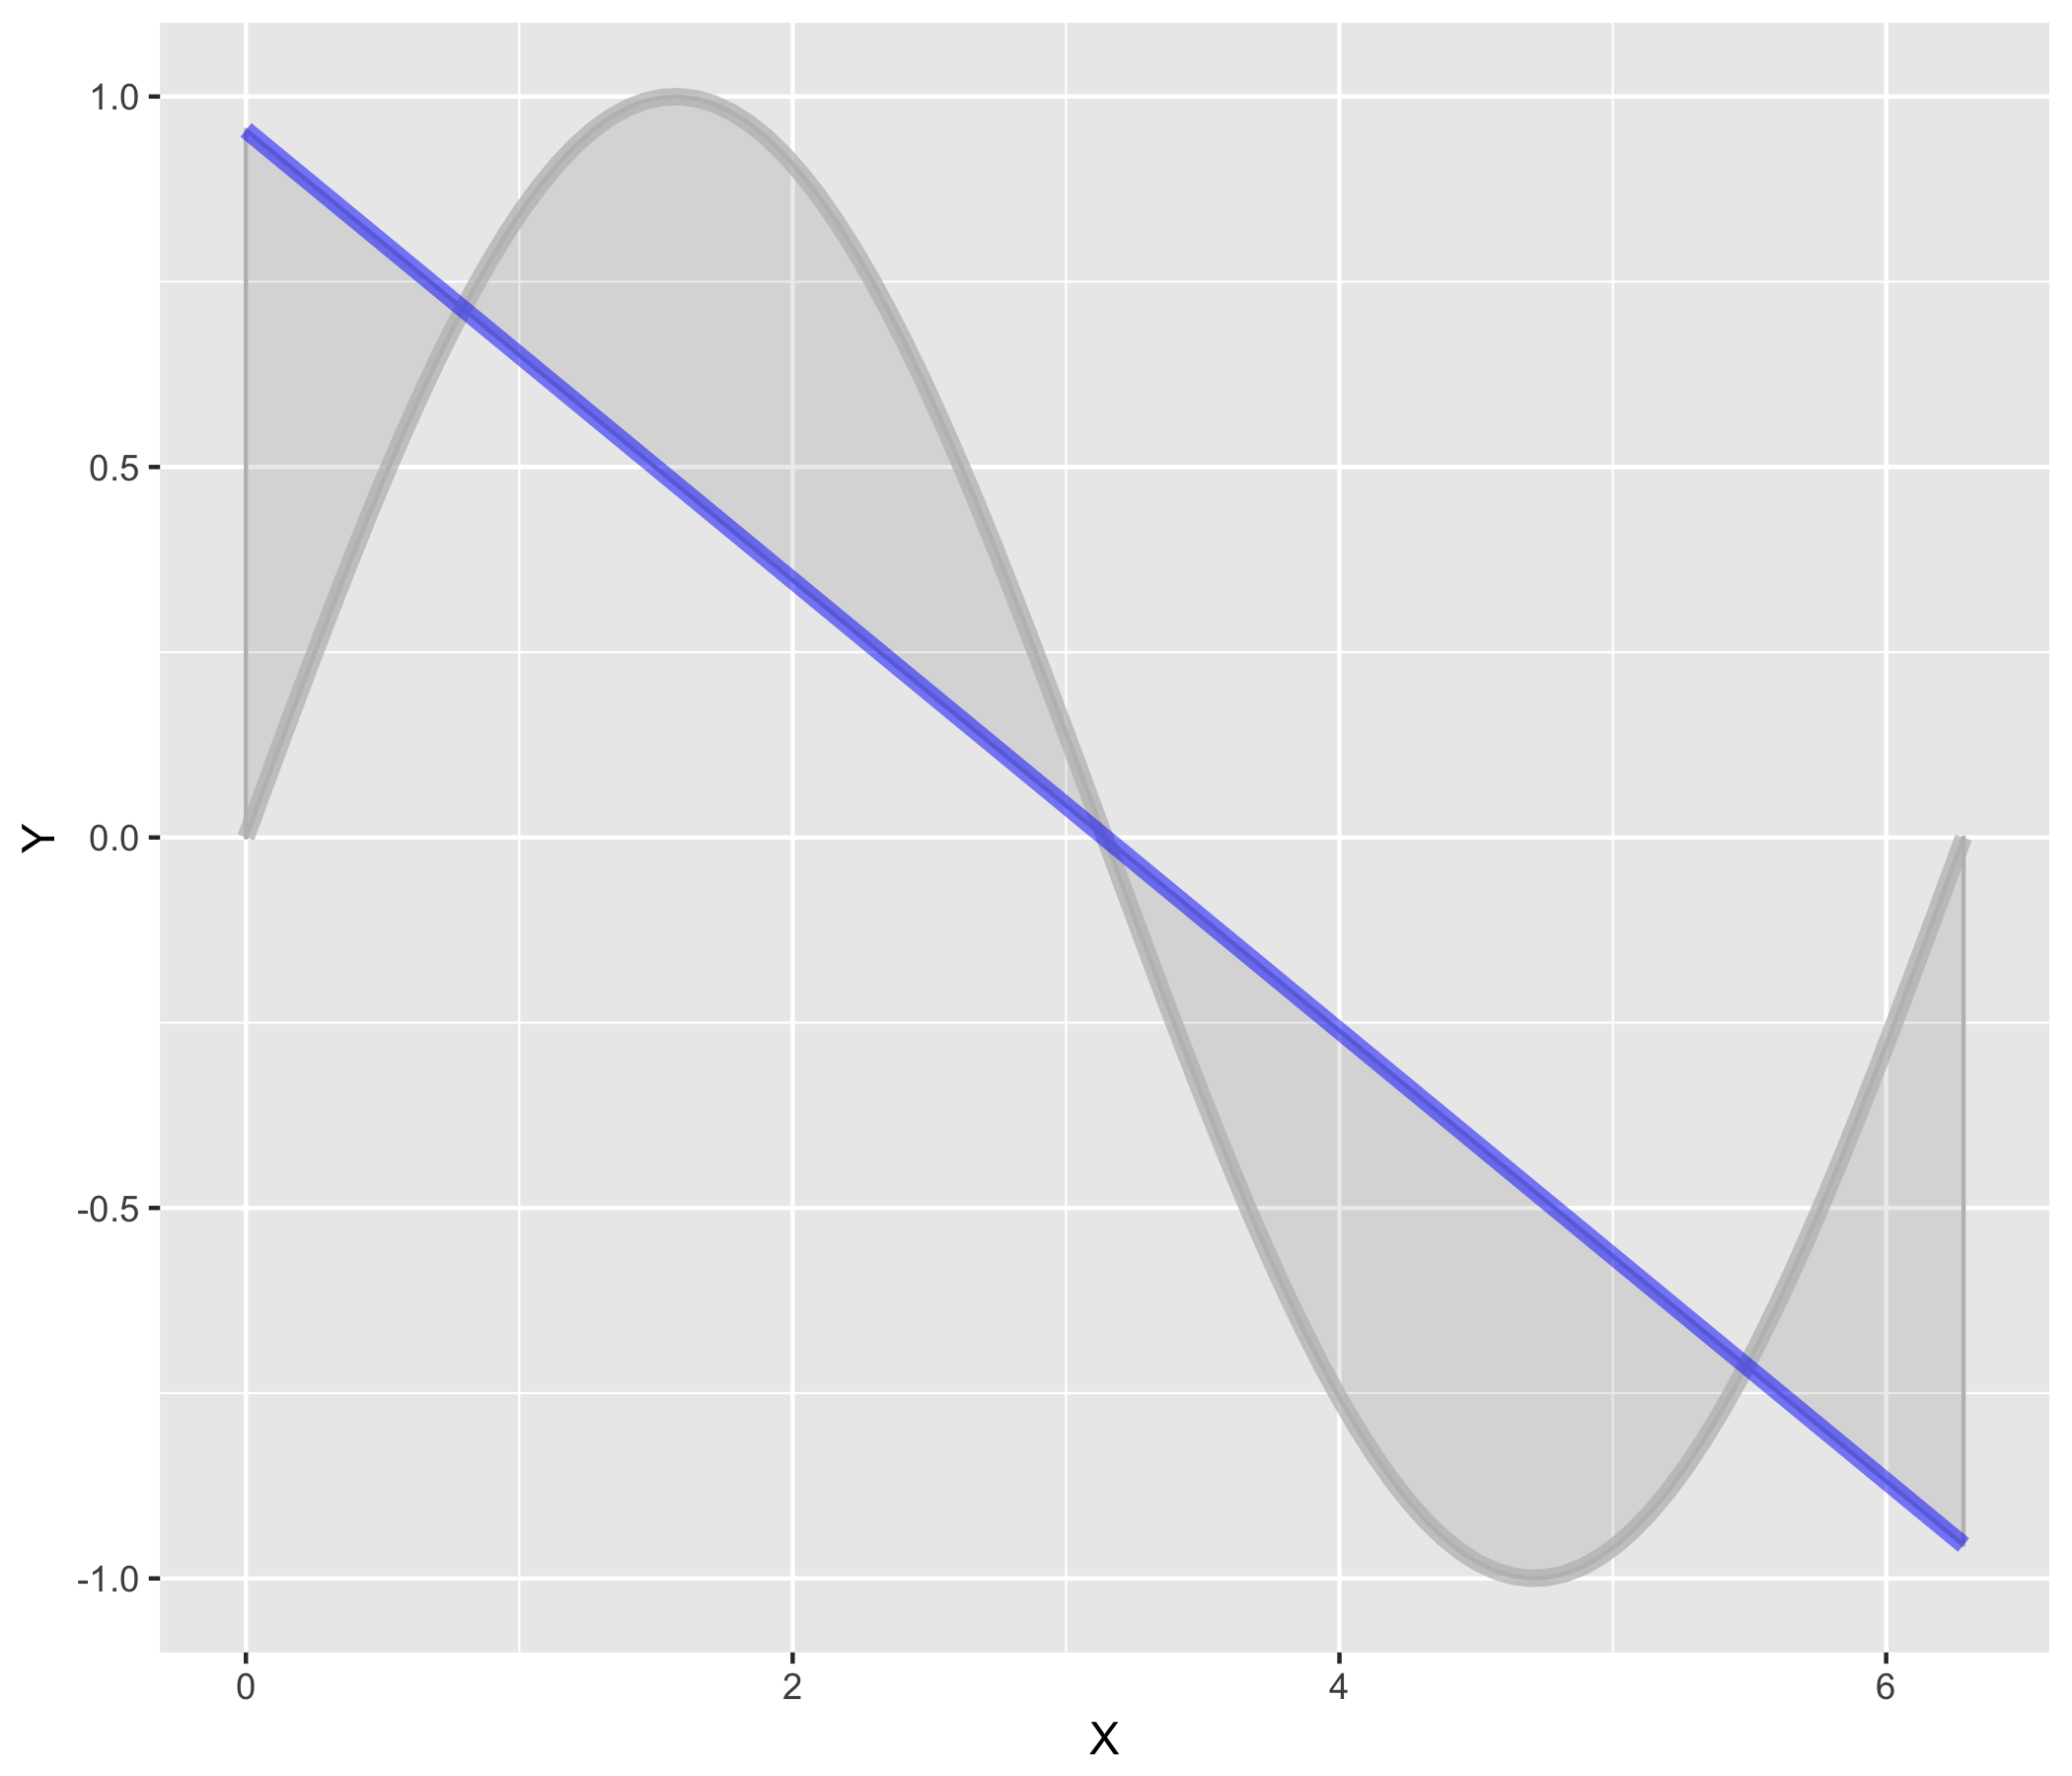
\includegraphics[scale=0.08]{model_bias}
  \end{figure}
\end{frame}
%
%
\begin{frame}
  The total bias can be explicitly calculated in this case (I used a numerical
  integration routine):
  $$ {\BIAS}^2 = E_X \left[ \left( \F(x) - Ef(x) \right)^2 \right] \approx 1.23
  $$
\end{frame}
%
%
\begin{frame}
  Bias can be lowered by making our learning algorithm more complex.  For
  example, fitting a \textit{cubic} regression lowers the bias of our model
  considerably:
  \begin{figure}
    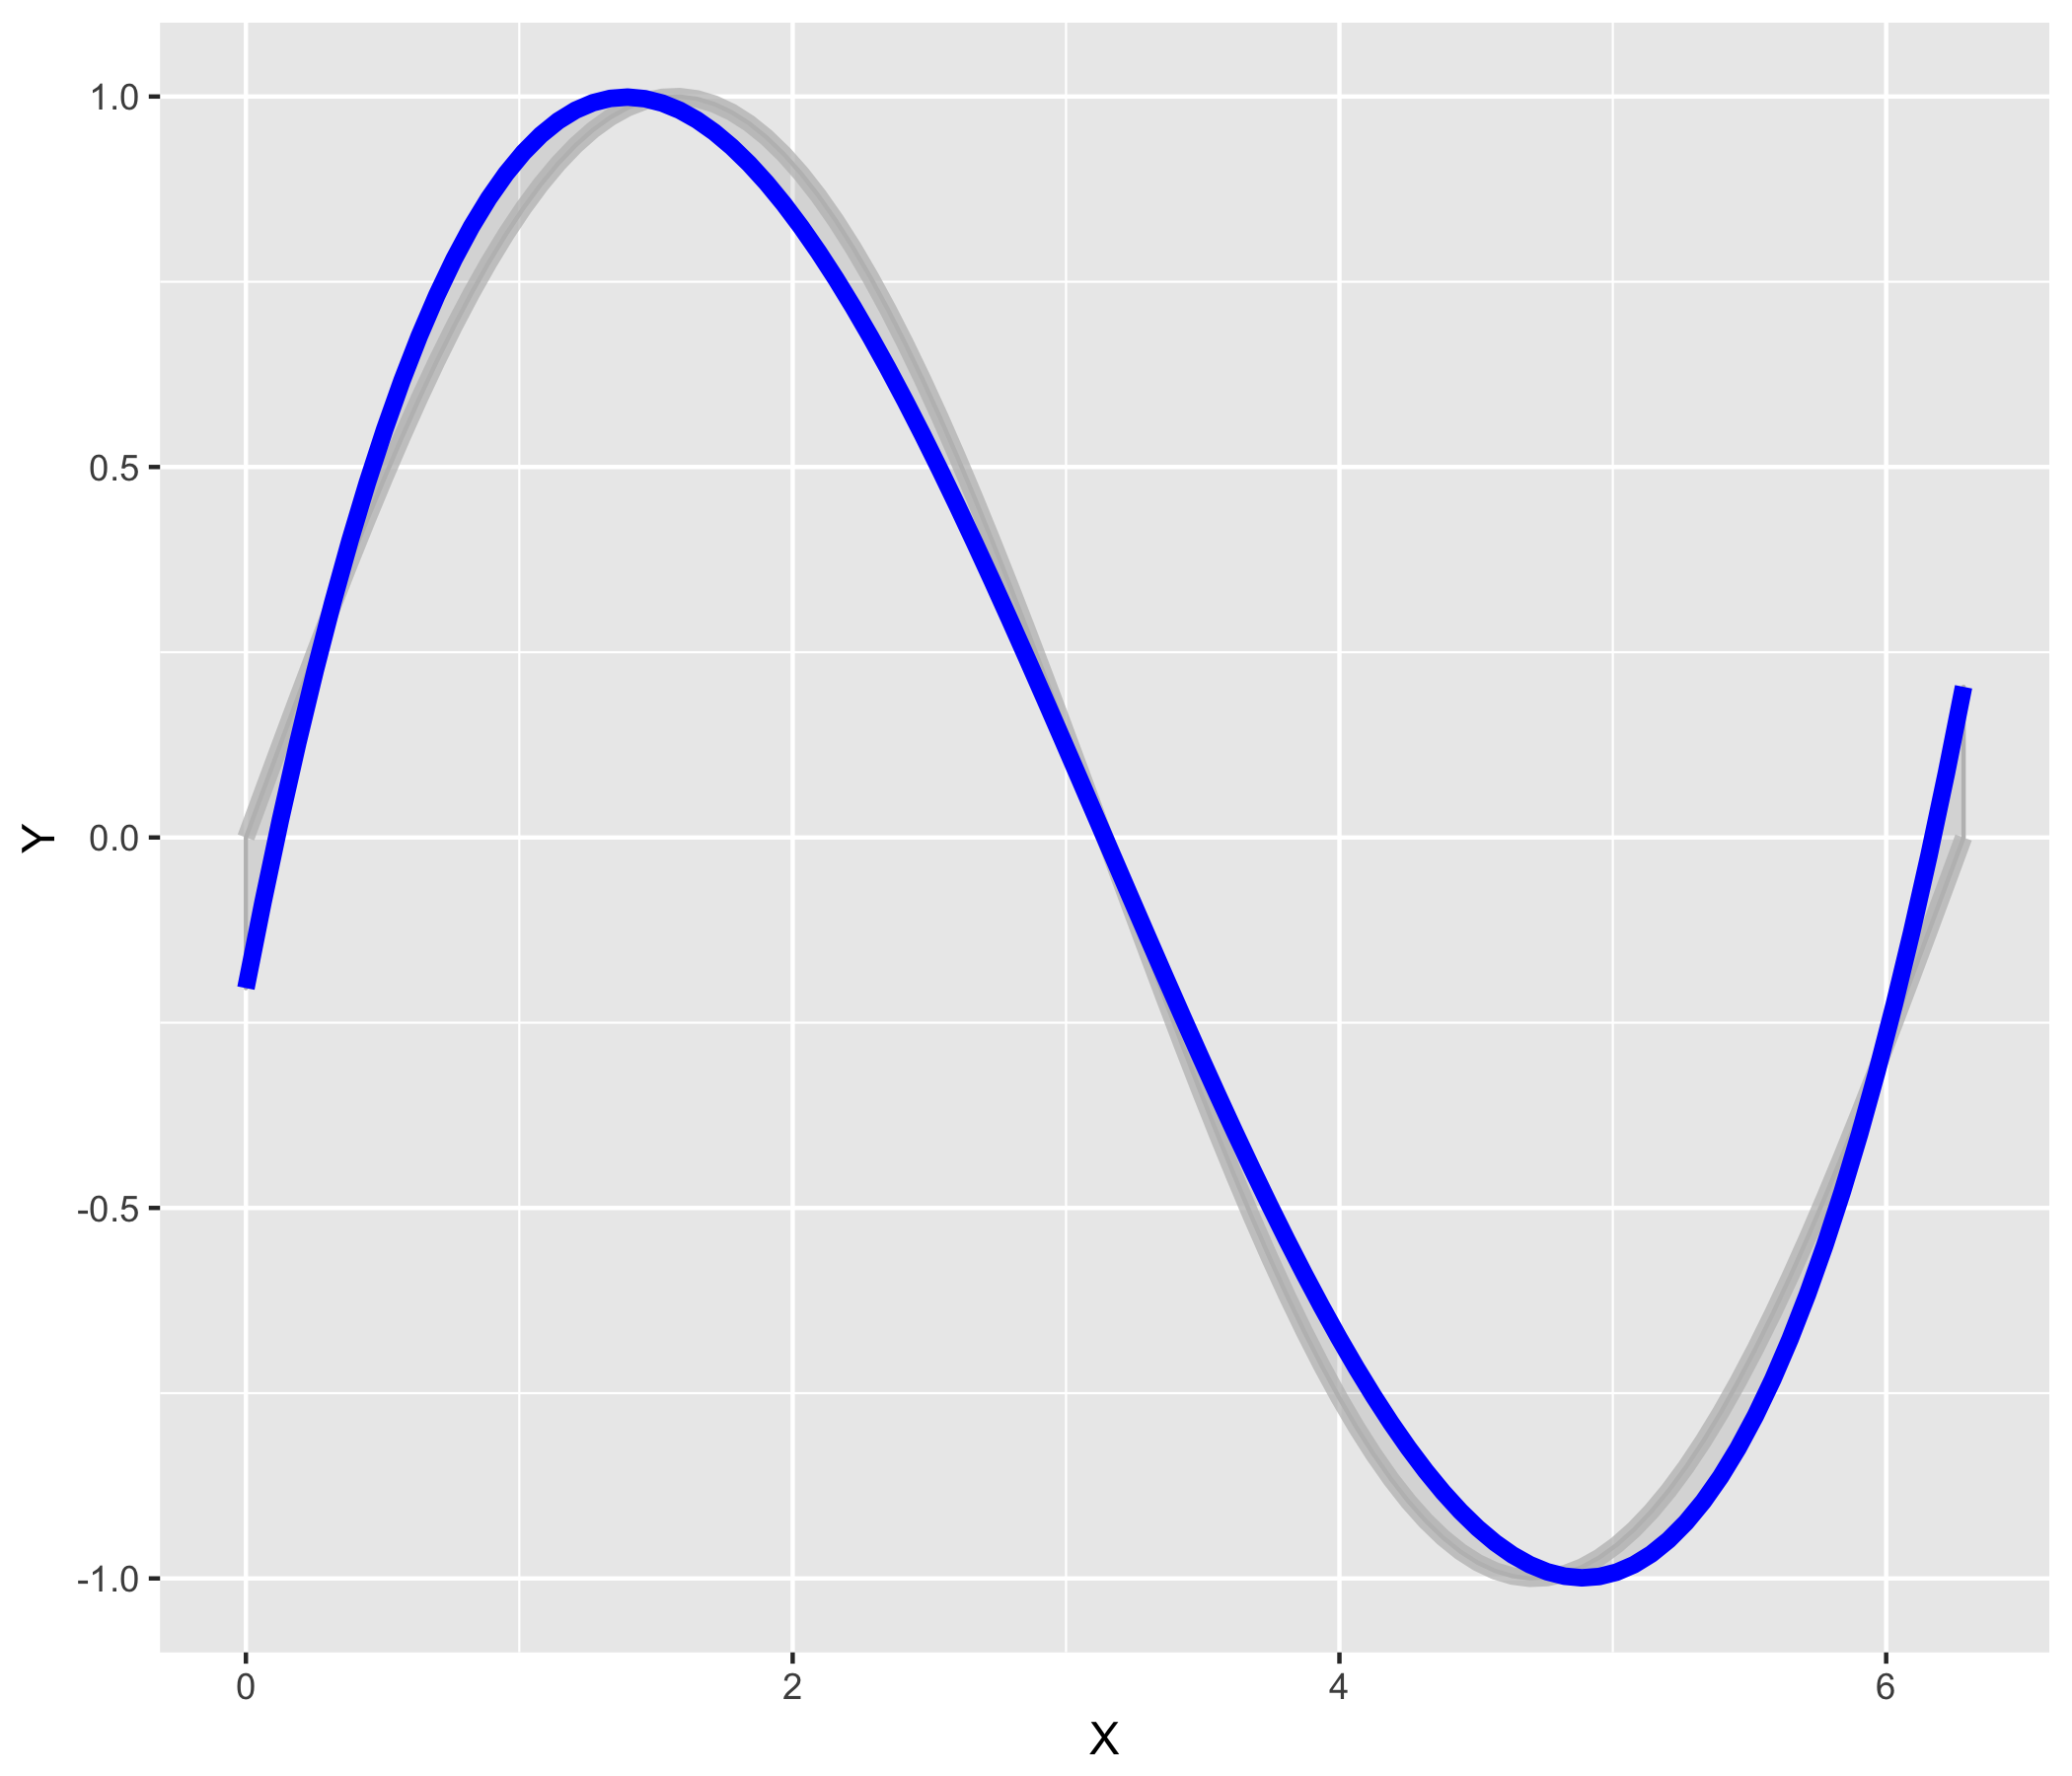
\includegraphics[scale=0.08]{cubic_model_bias}
  \end{figure}
  $$ {\BIAS}^2 = E_X \left[ \left( \F(x) - Ef(x) \right)^2 \right] \approx 0.028
  $$
\end{frame}
%
%
\begin{frame}
  It is tempting to want to lower the bias as much as possible, as this brings
  our expected model close to reality, unfortunately, the model variance is a
  price we pay.
\end{frame}
%
%
\begin{frame}
  The model variance measures how sensitive our estimate is to the specific
  training data used:
      $$ E_{\D} \left[ \left( Ef(x) - f(x,\D) \right)^2 \mid x \right] $$
\end{frame}
%
%
\begin{frame}
   Lines fit to different data sampled from our model distribution tend to
   cluster around the best linear fit, but there is a fair amount of variance in
   the clustering:
  \begin{figure}
    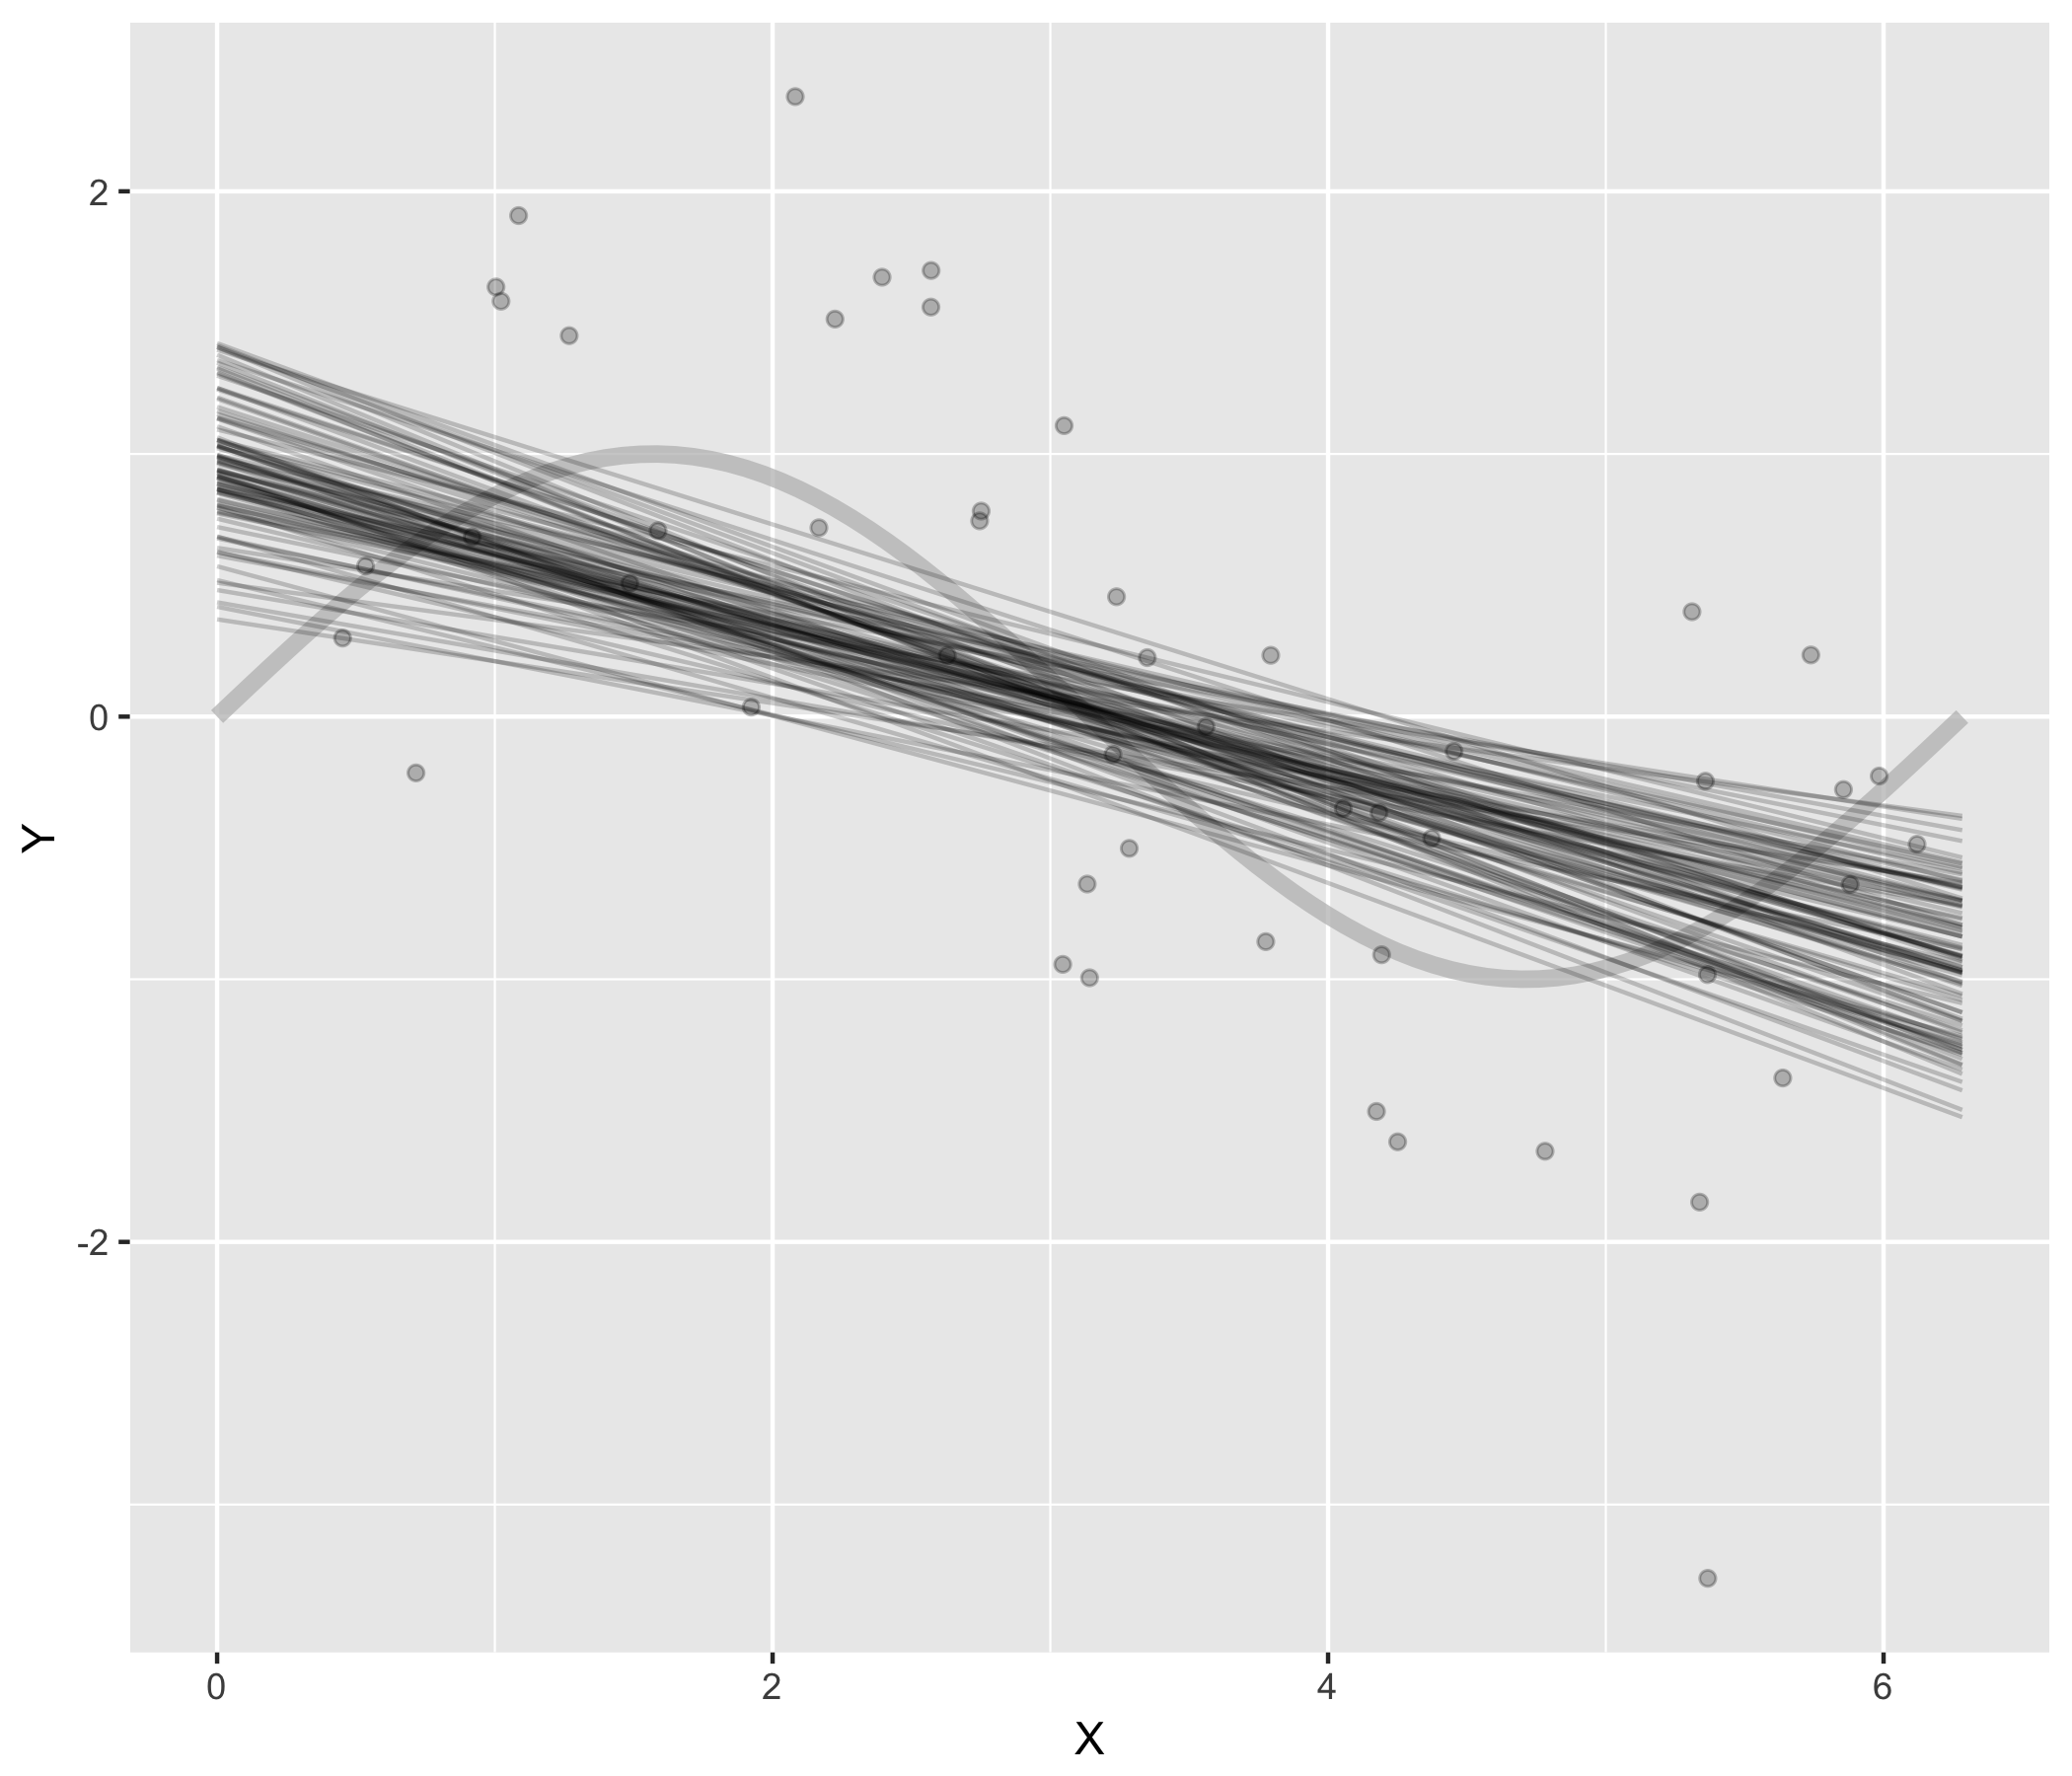
\includegraphics[scale=0.09]{model_variance_standard_samples}
  \end{figure}
\end{frame}
%
%
\begin{frame}
  Increasing the amount of data used to fit reduces the variance:
  \begin{figure}
    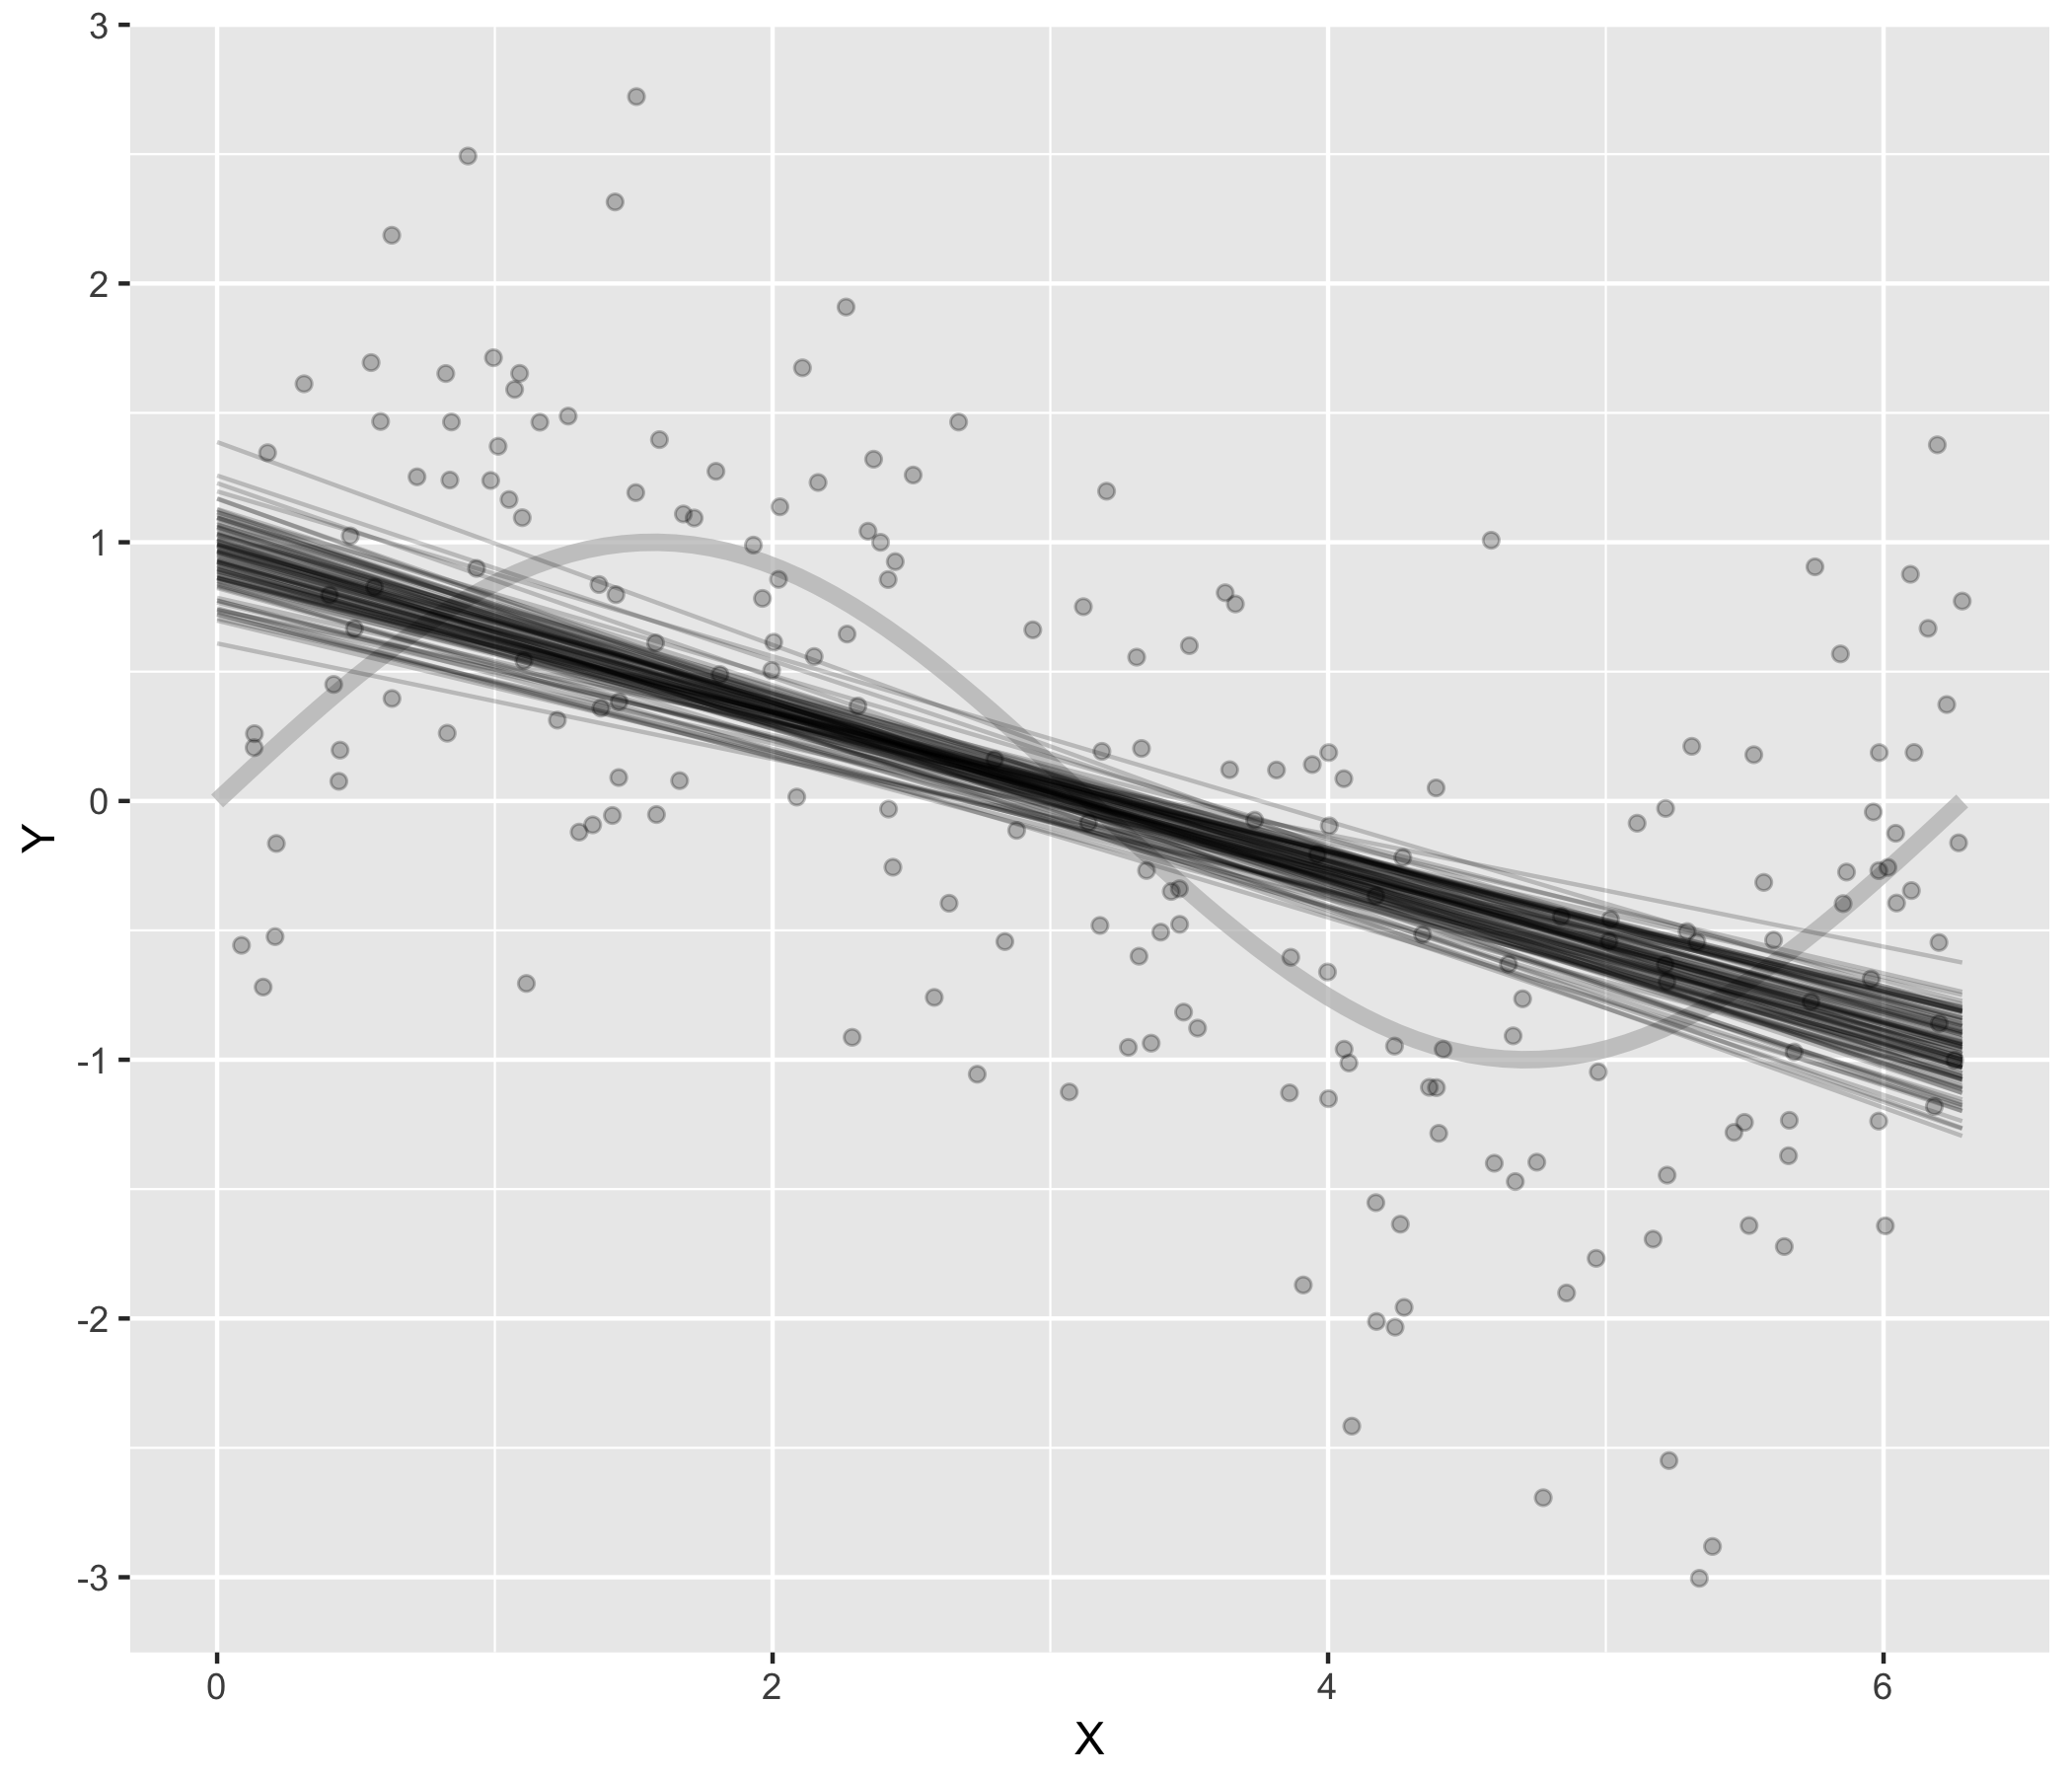
\includegraphics[scale=0.09]{model_variance_more_samples}
  \end{figure}
\end{frame}
%
%
\begin{frame}
  Decreasing the amount of data used to fit increases the variance:
  \begin{figure}
    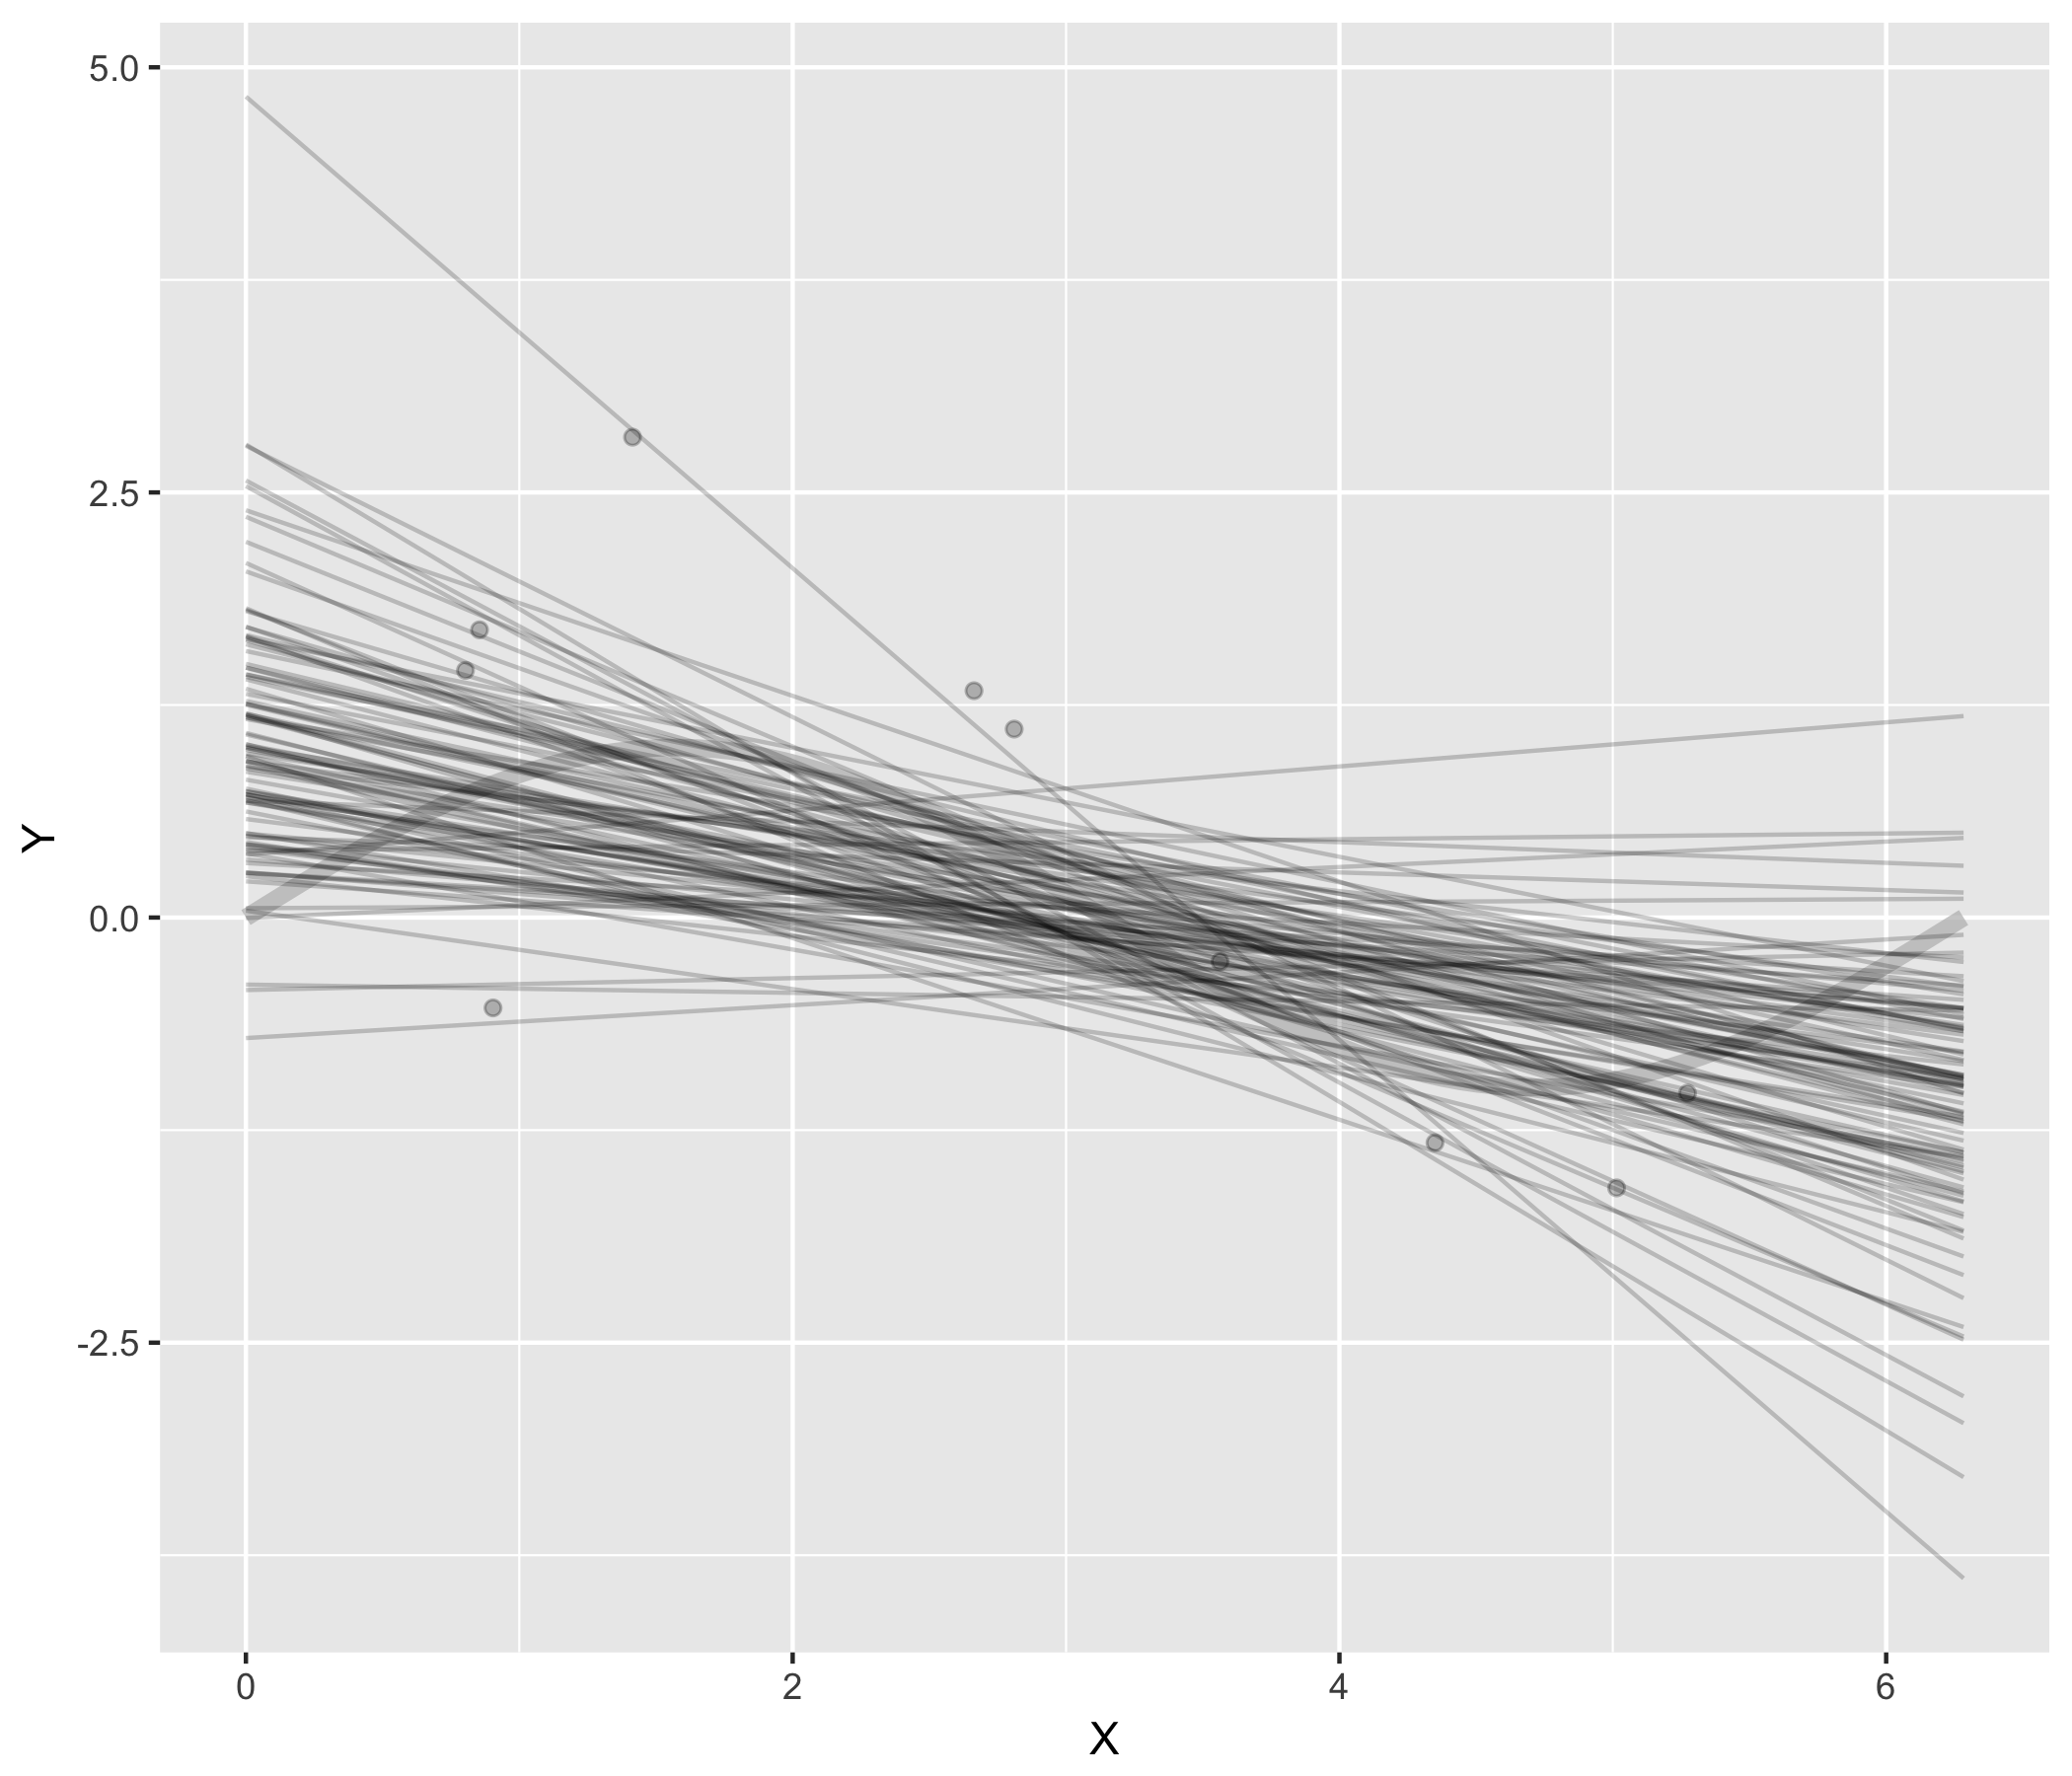
\includegraphics[scale=0.09]{model_variance_less_samples}
  \end{figure}
\end{frame}
%
%
\begin{frame}
  As the amount of data available for training is increased, estimates of
  expected error tend to approach a limit after which they cannot be decreased:
  \begin{figure}
    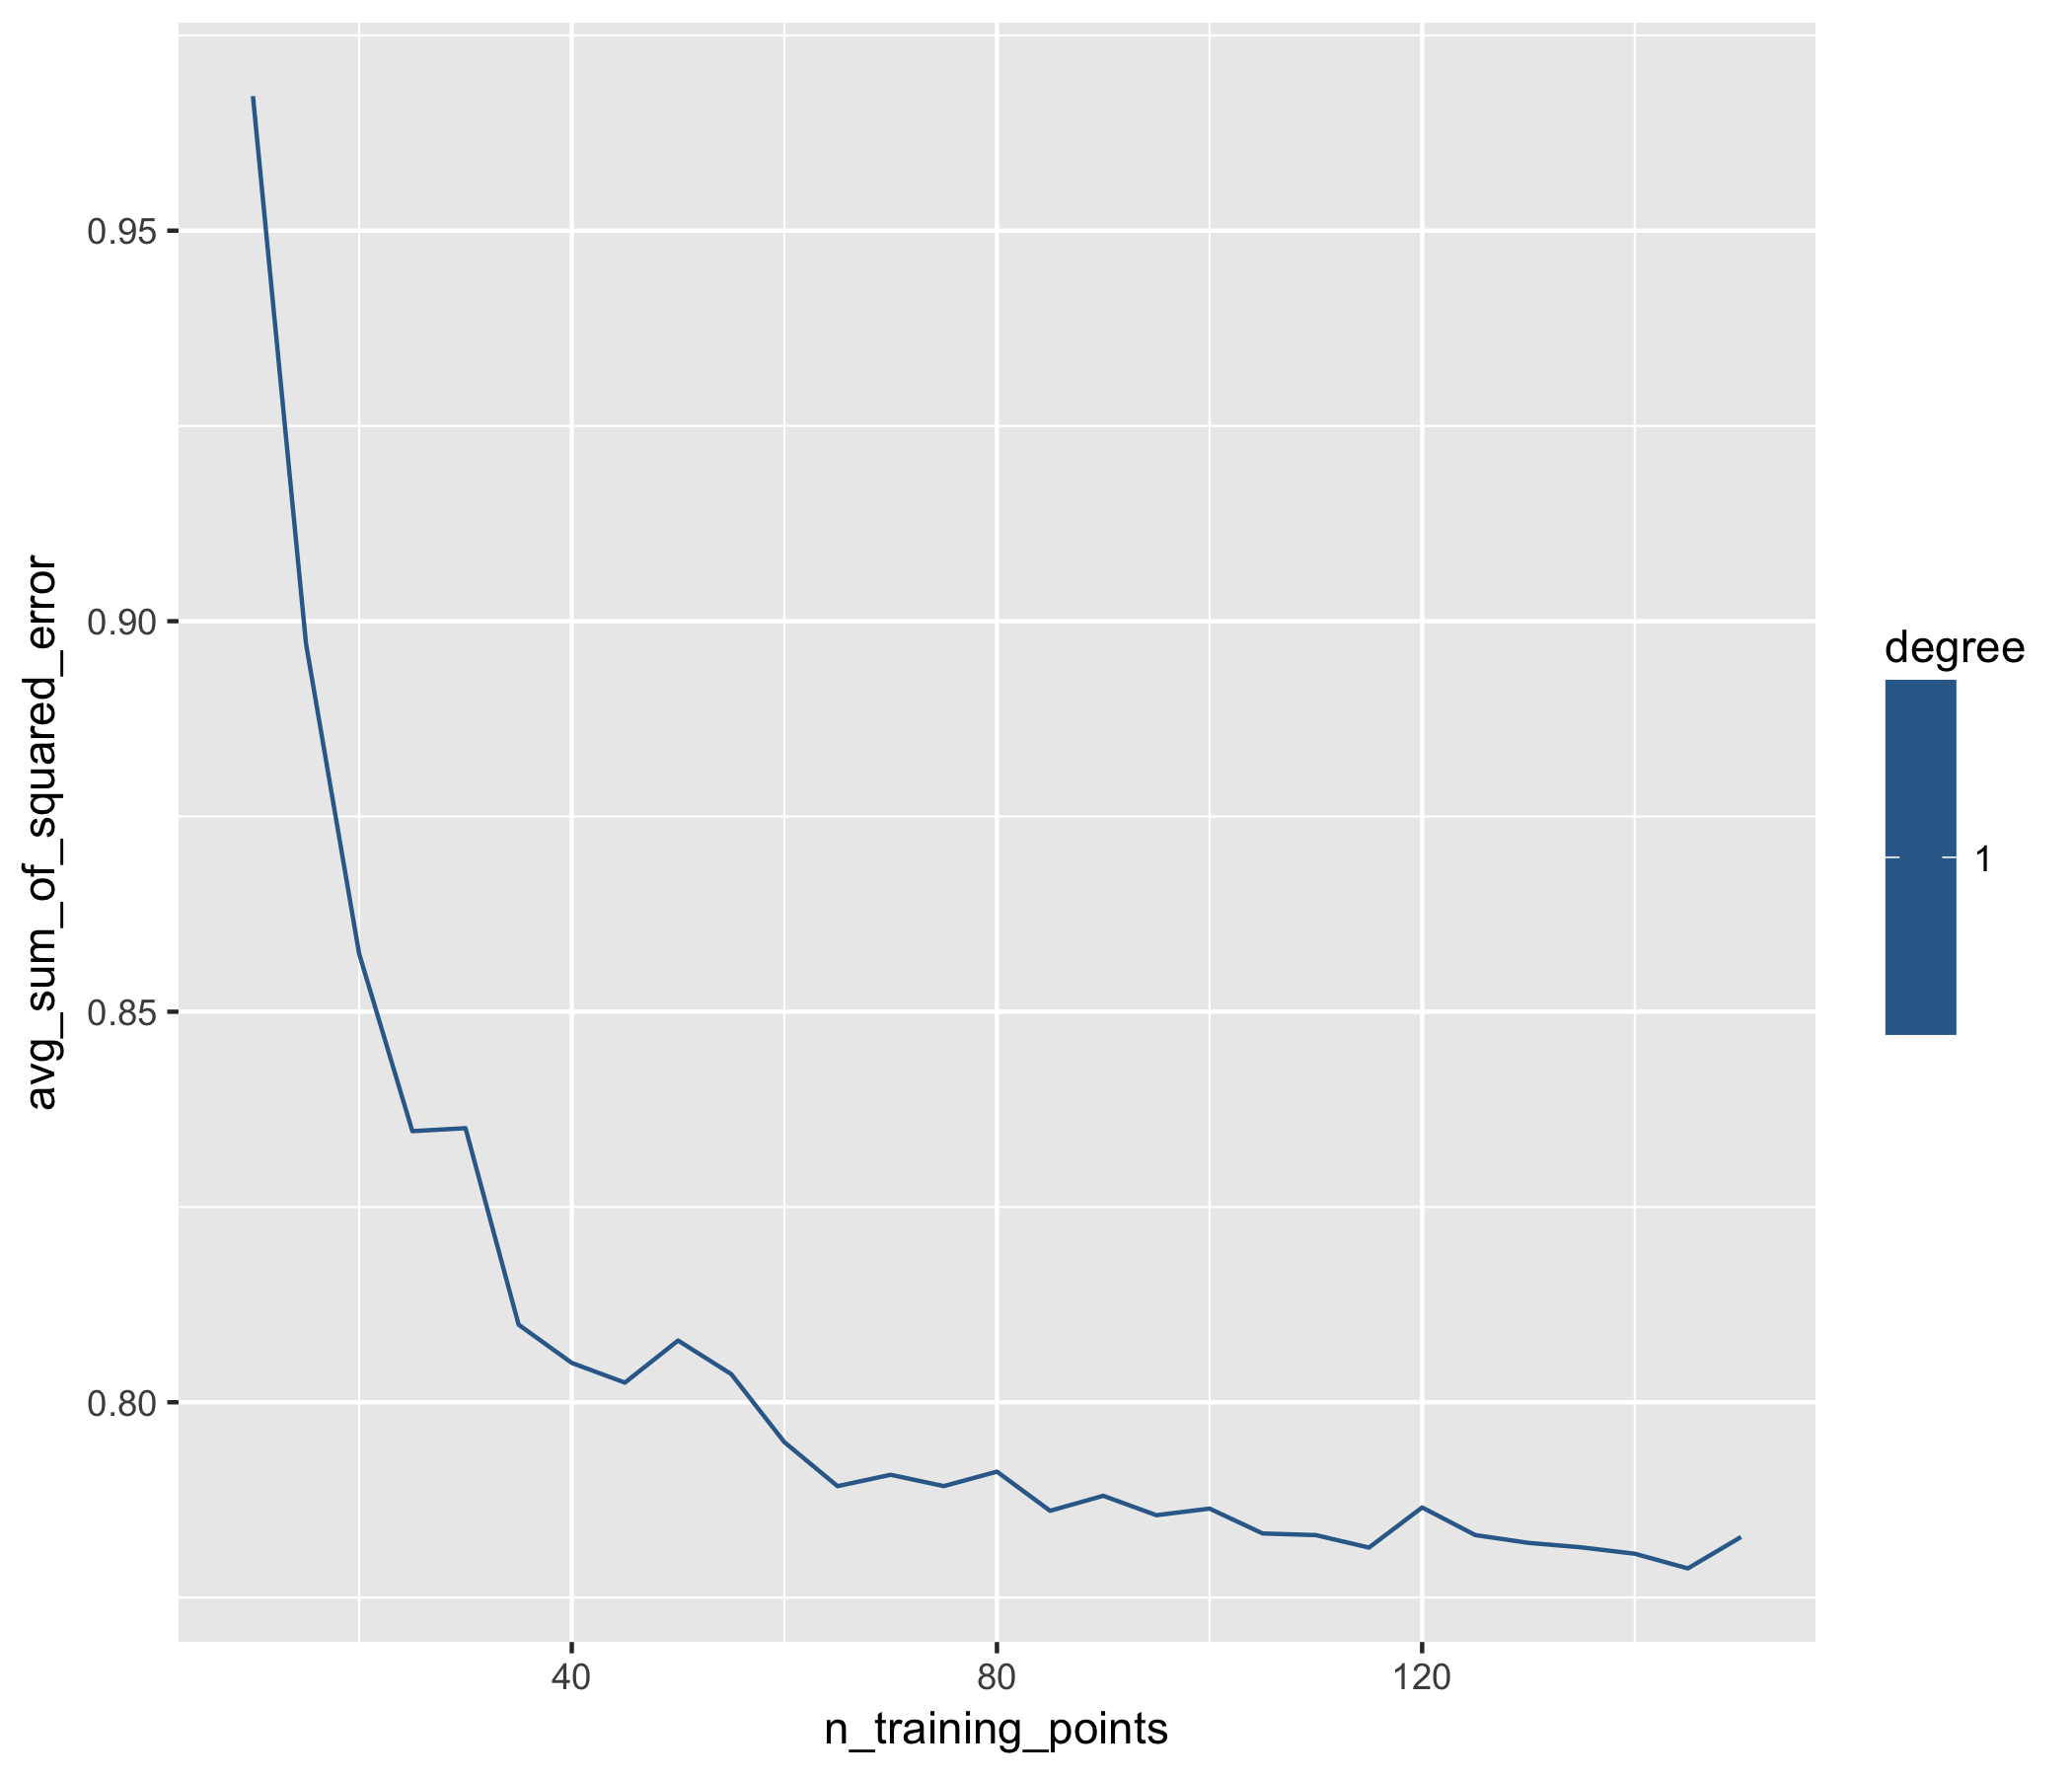
\includegraphics[scale=0.09]{out_of_sample_learning_curve}
  \end{figure}
\end{frame}
%
%
\begin{frame}
  The error remaining after the estimate stabilizes are due to the other error
  components: the irreducible error and the model bias.
  \begin{figure}
    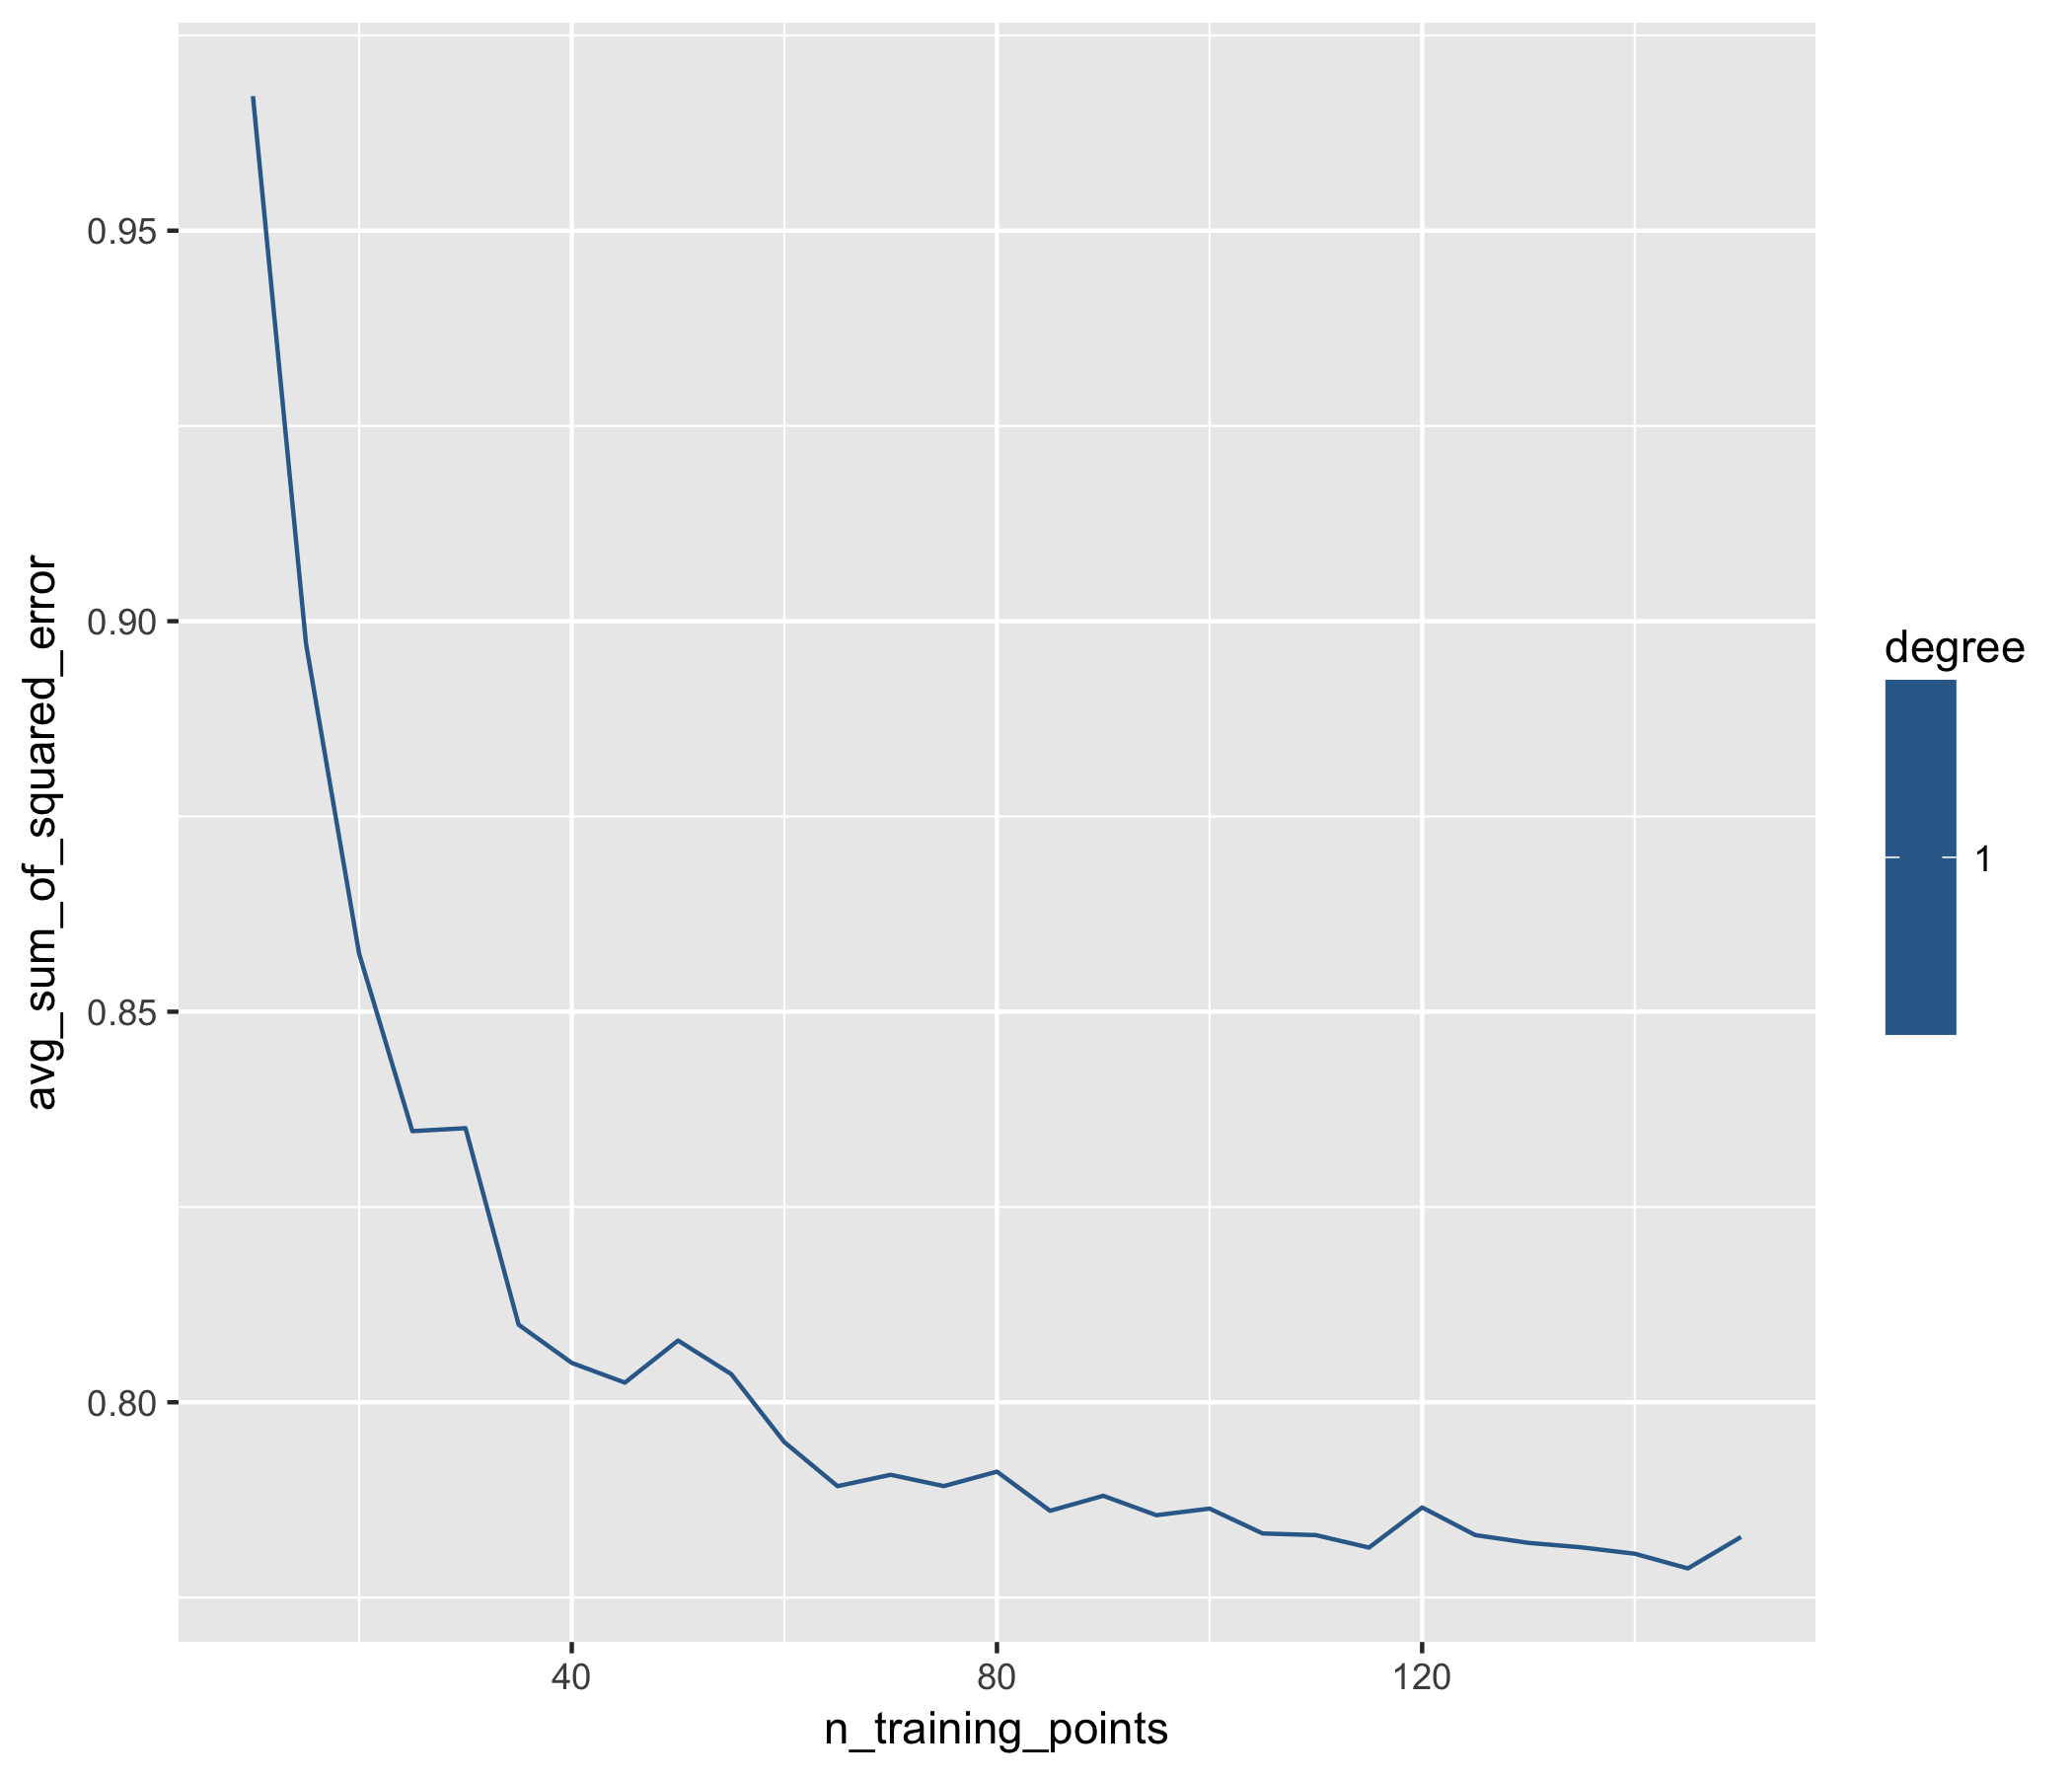
\includegraphics[scale=0.09]{out_of_sample_learning_curve}
  \end{figure}
\end{frame}
%
%
\begin{frame}
  Increasing the complexity of the model also tends to increase the model
  variance:
  \begin{figure}
      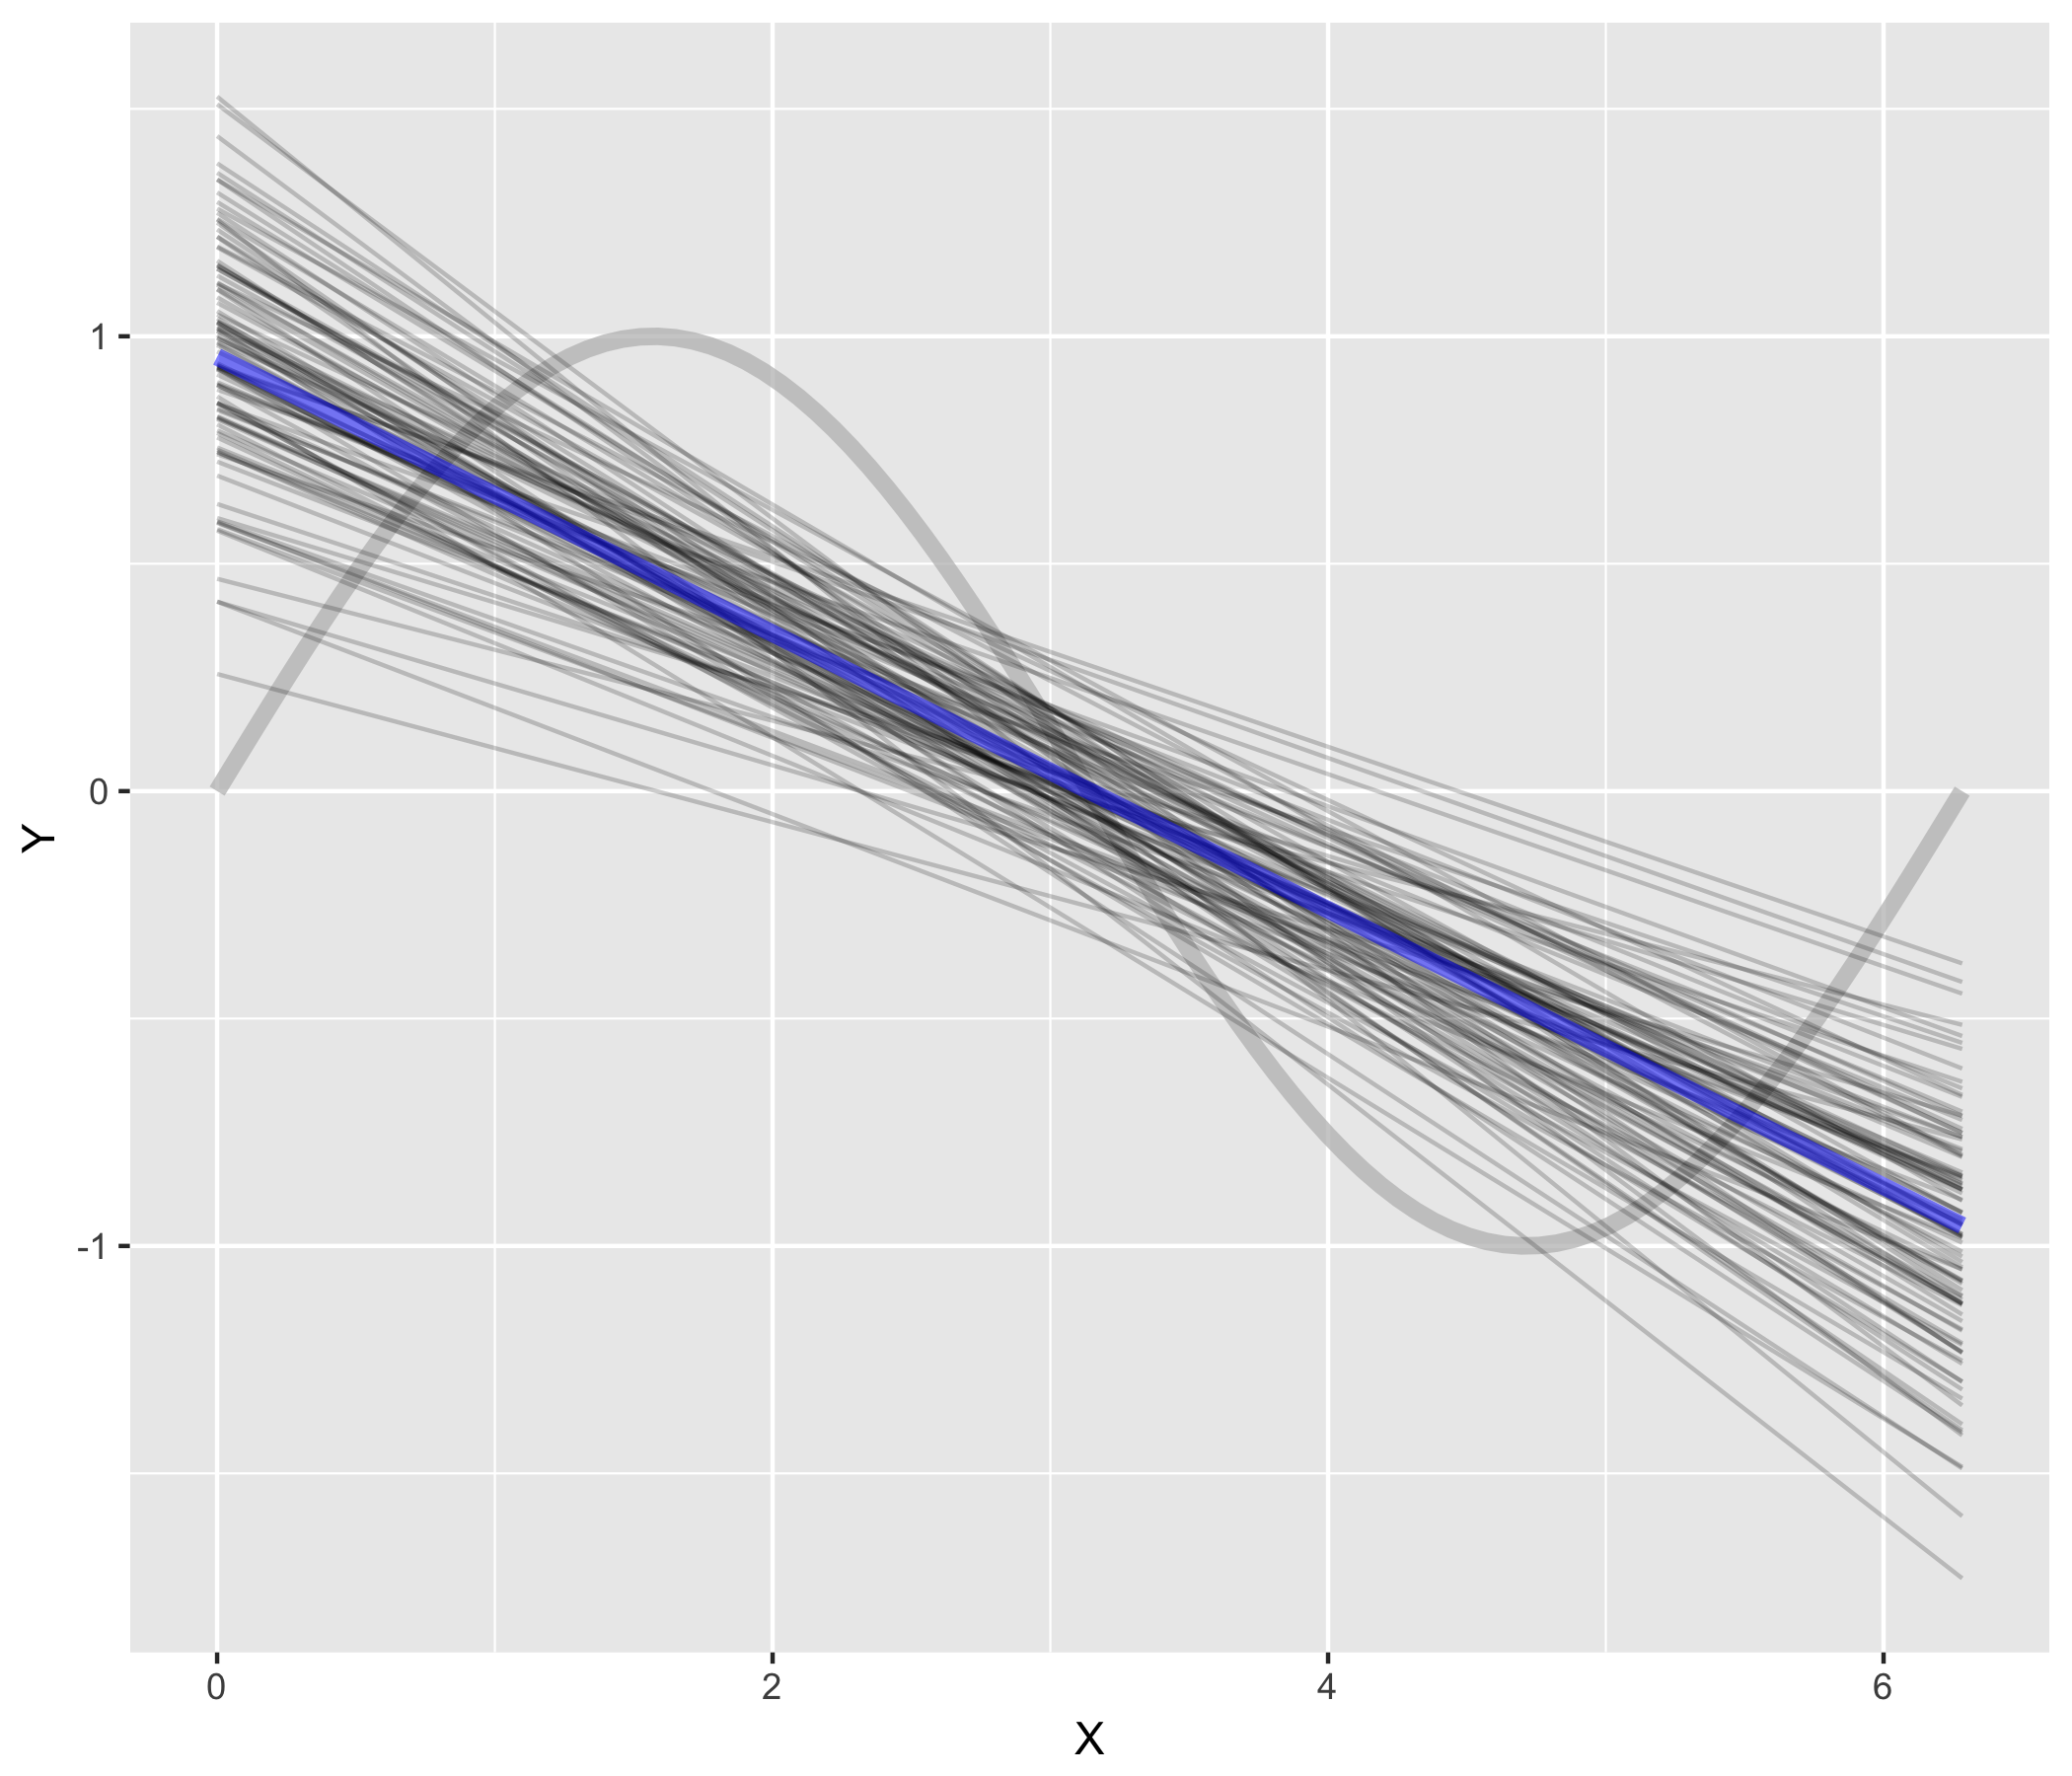
\includegraphics[scale=0.05]{model_variance}
      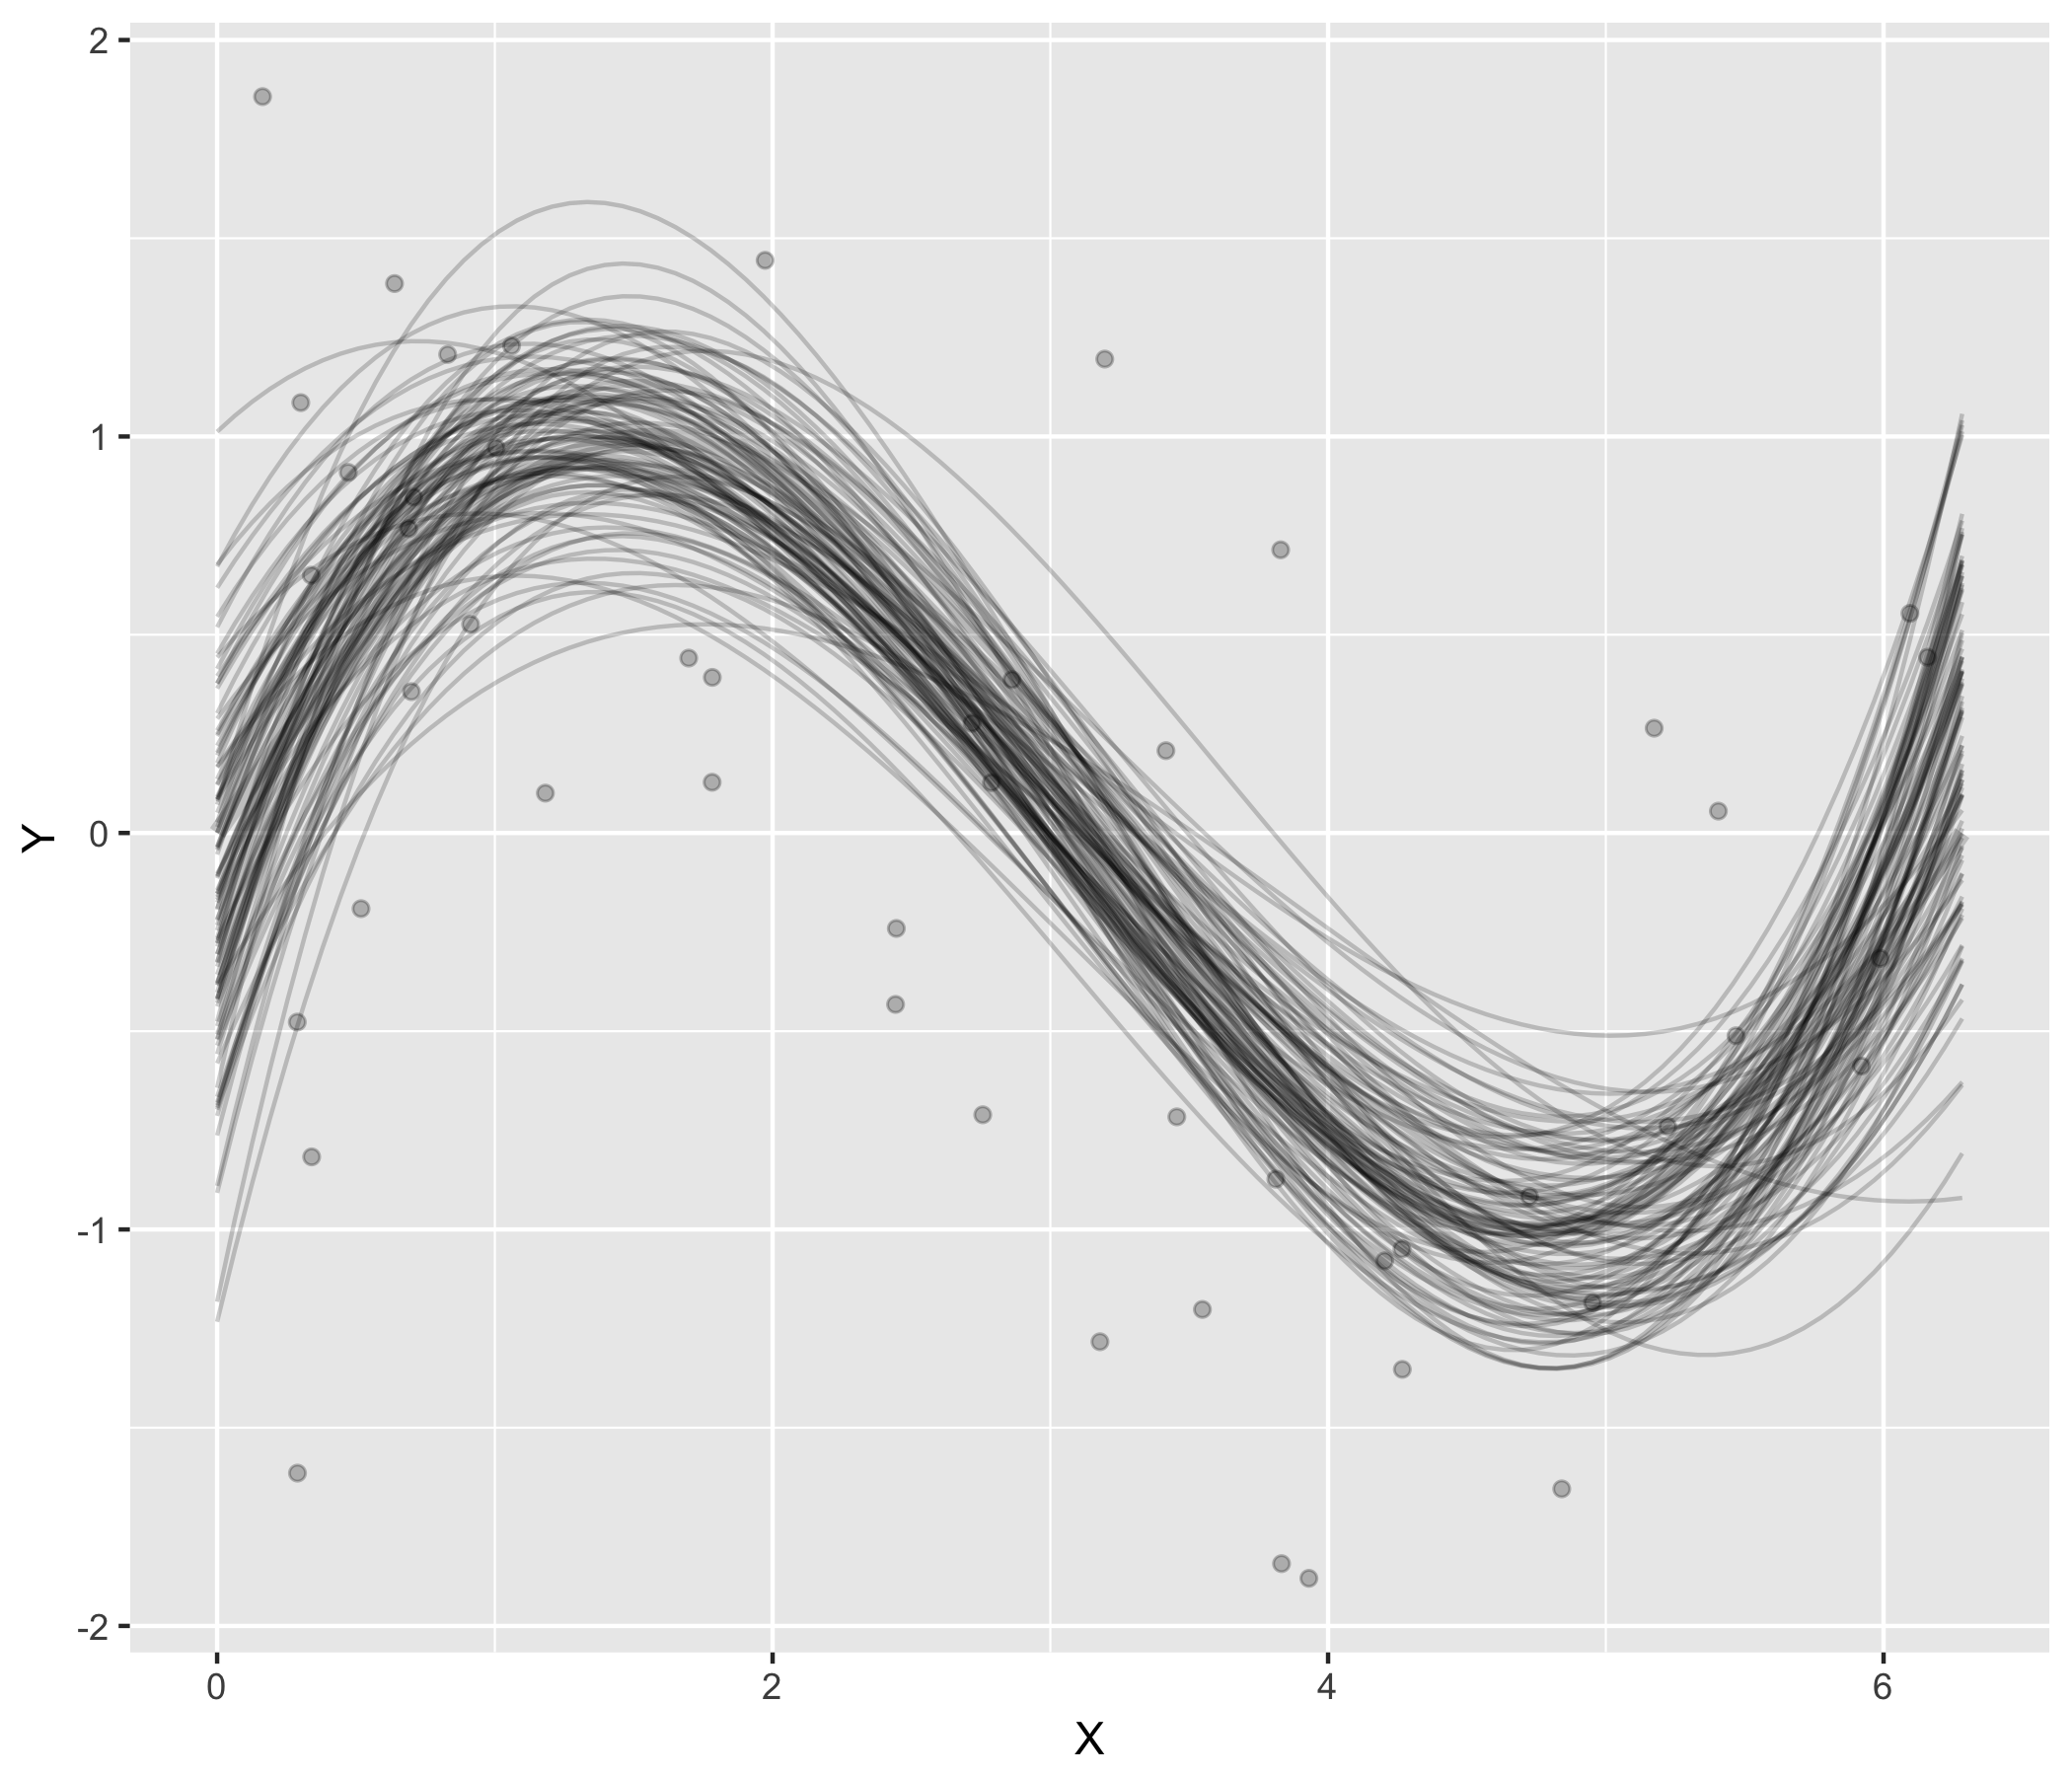
\includegraphics[scale=0.05]{model_variance_cubic}
  \end{figure}
  \begin{figure}
      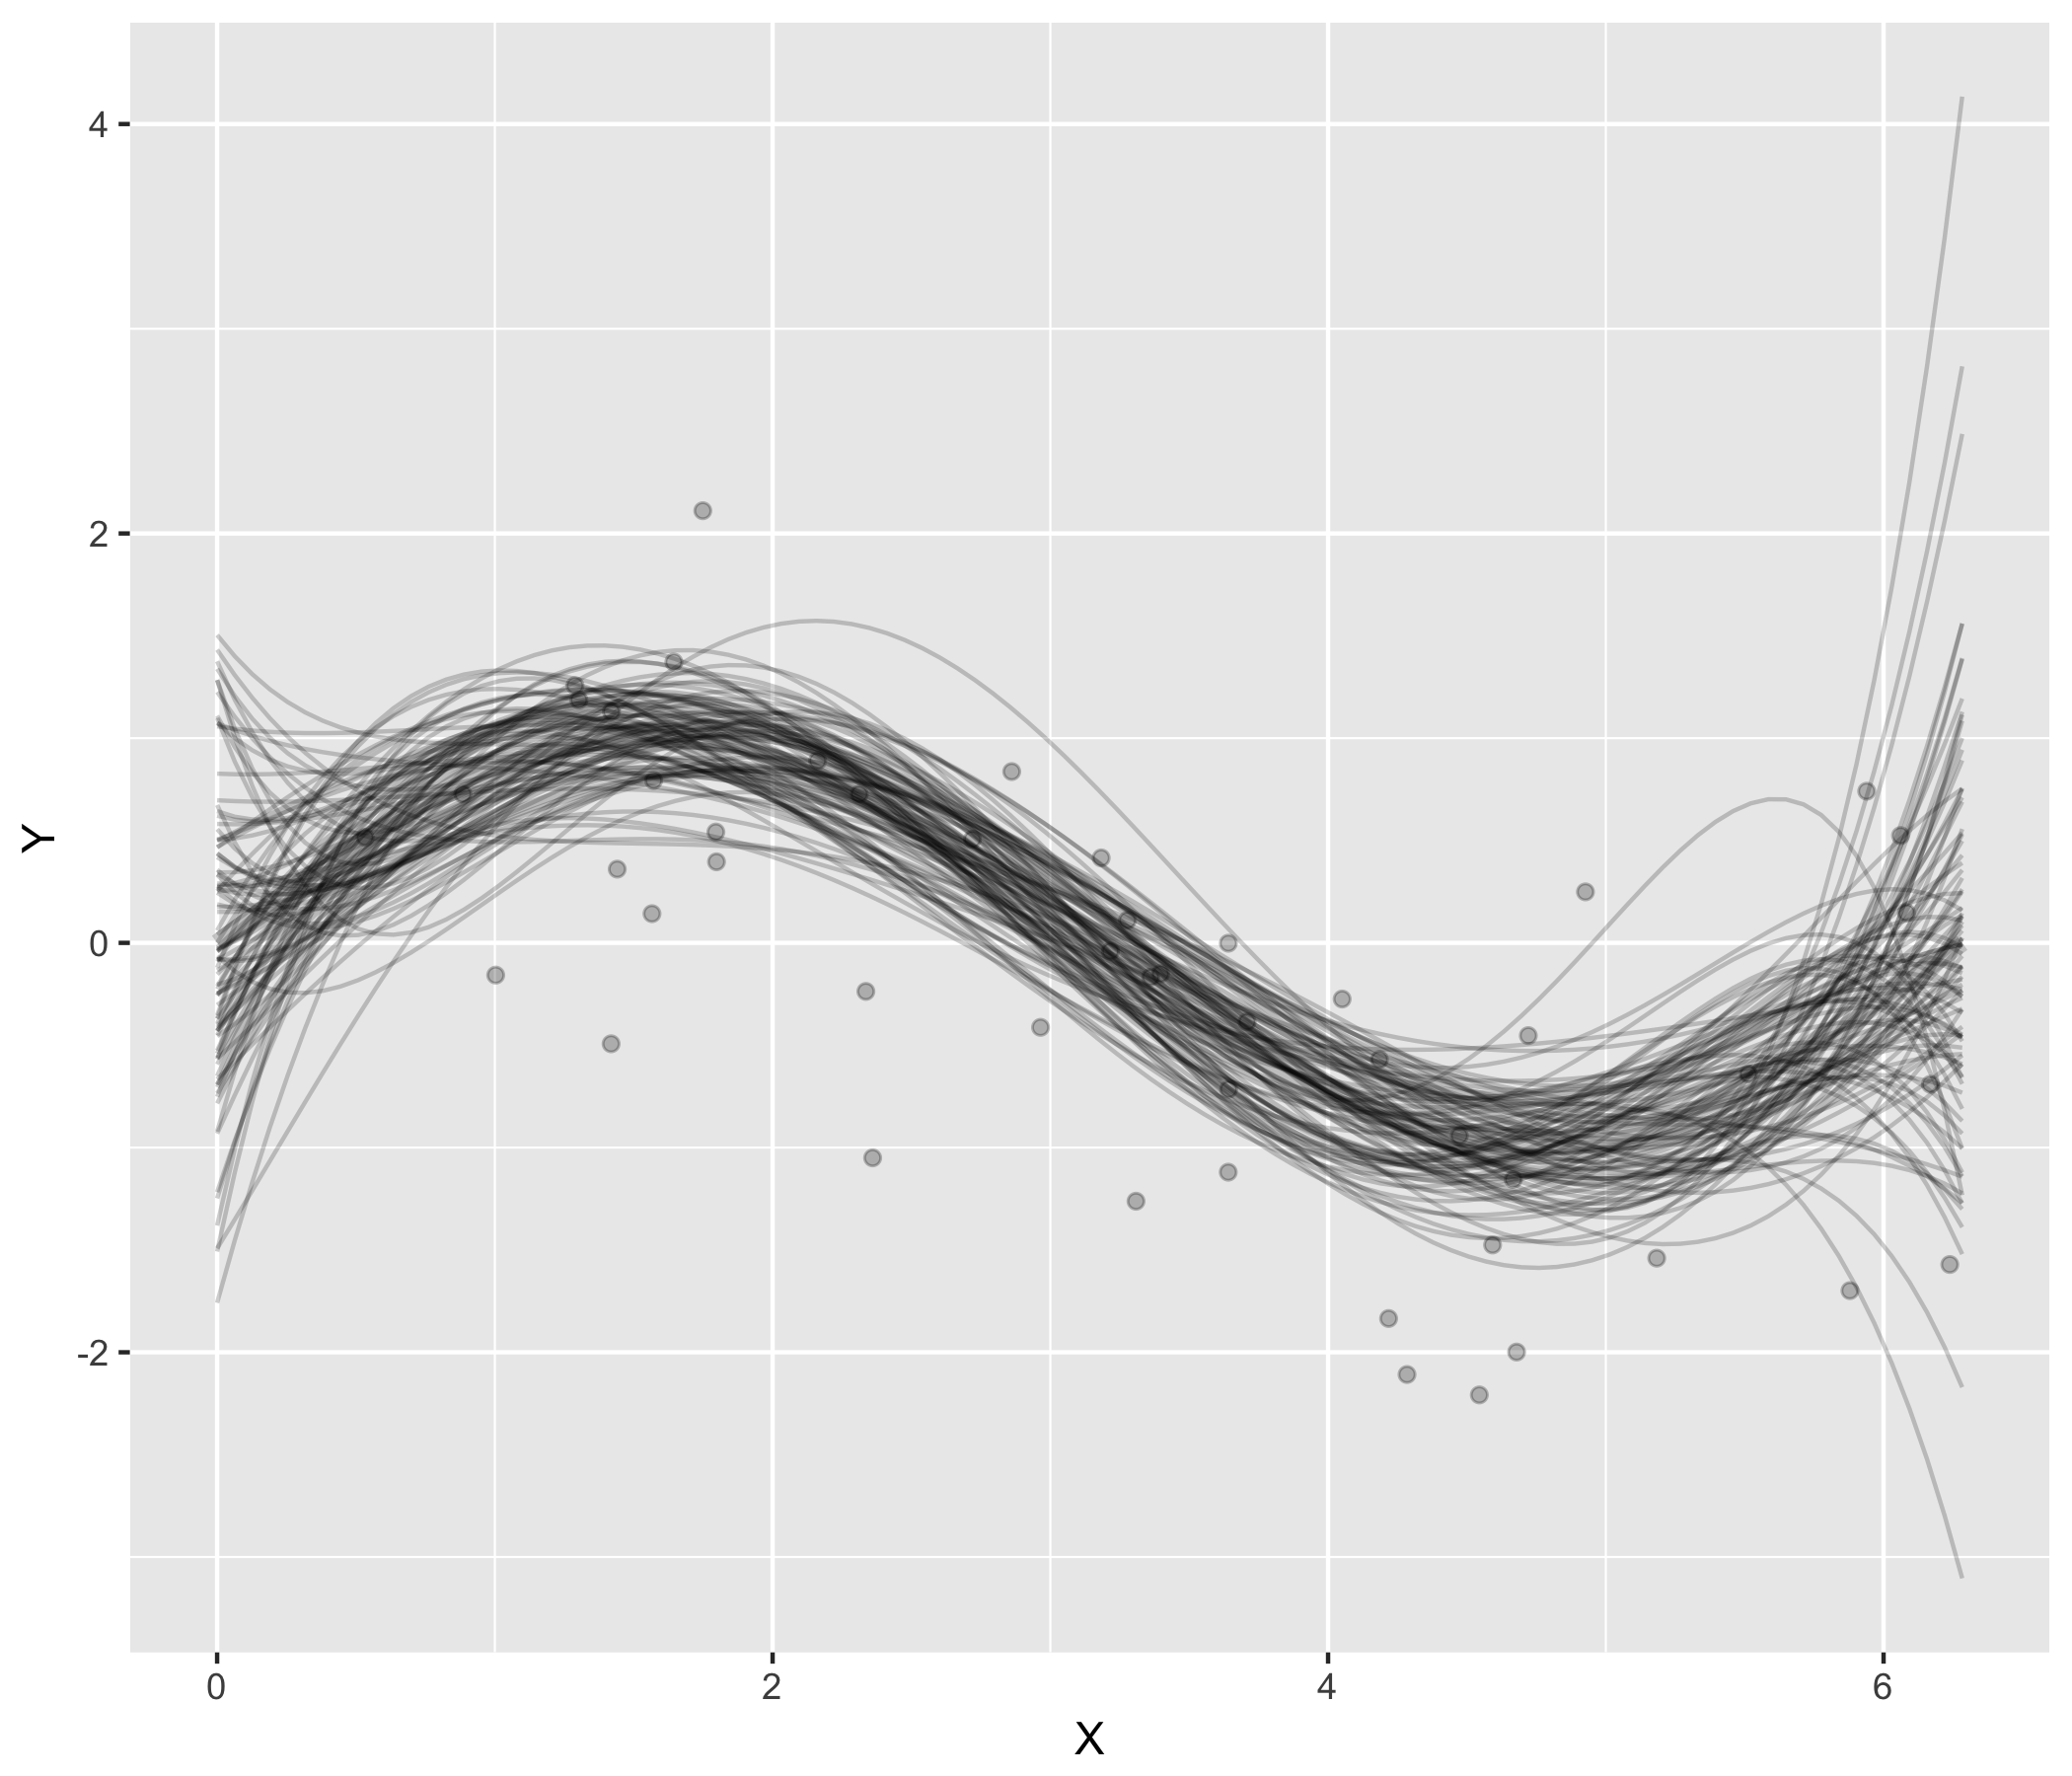
\includegraphics[scale=0.05]{model_variance_quartic}
      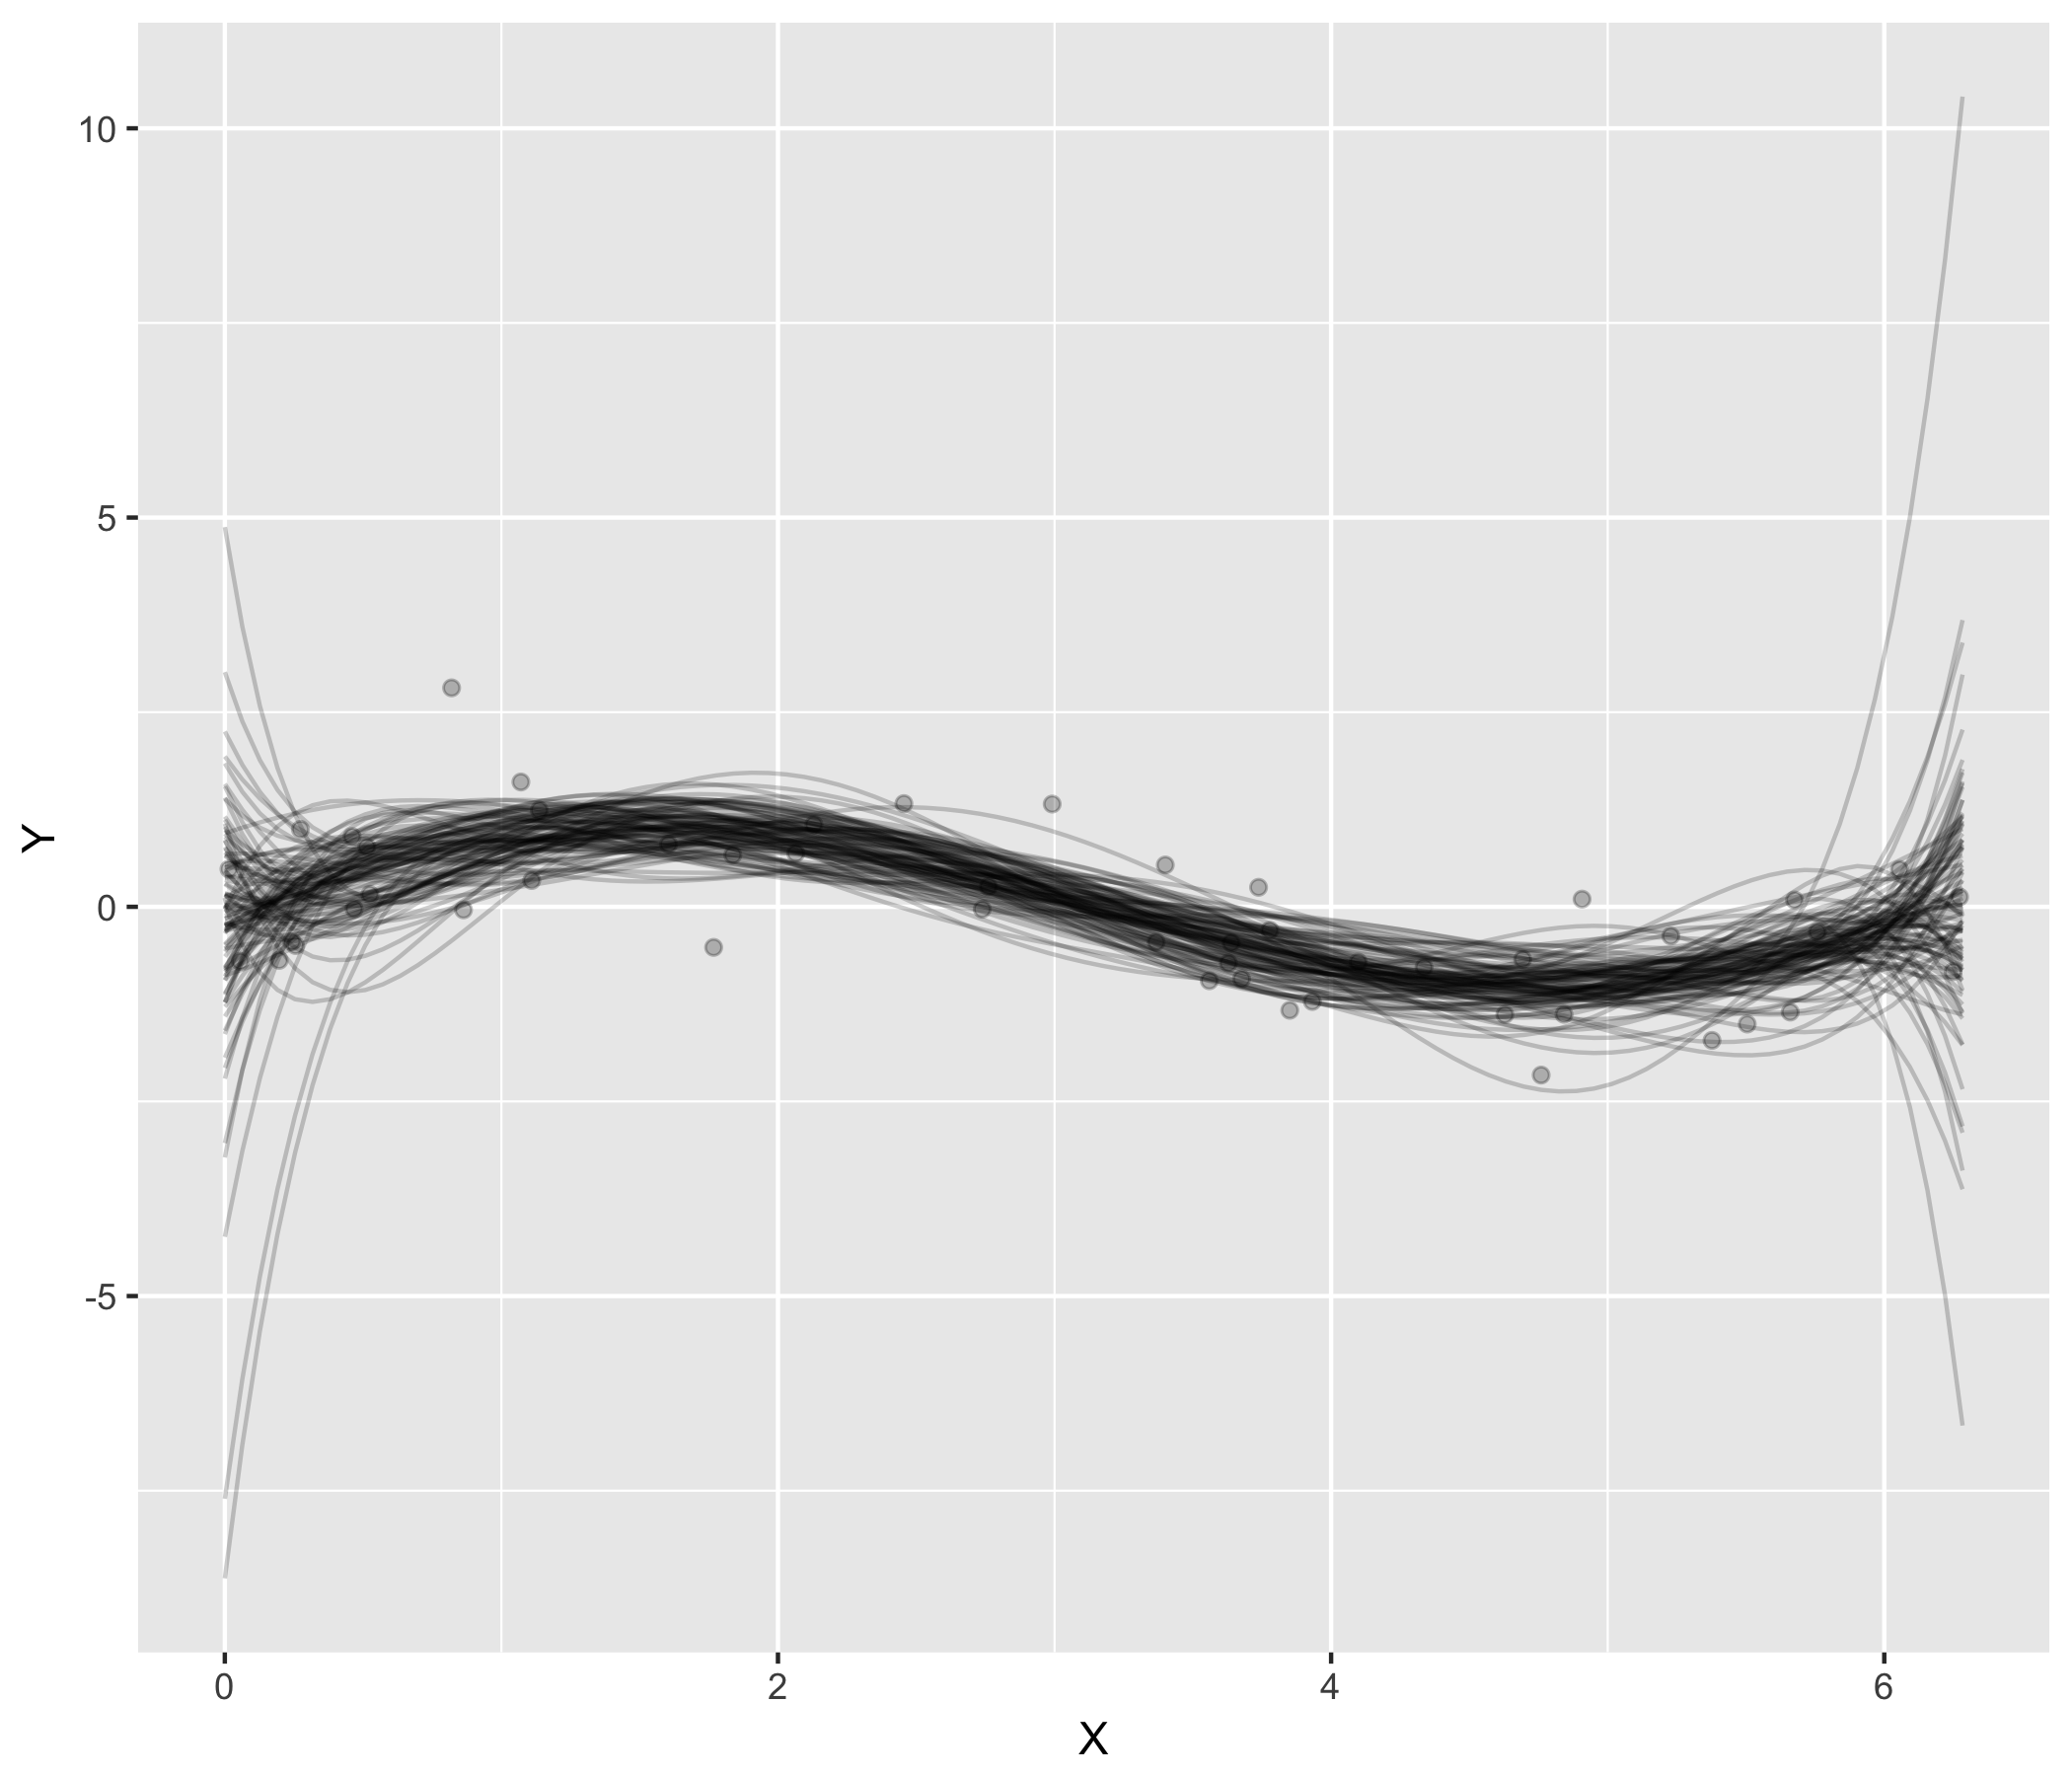
\includegraphics[scale=0.05]{model_variance_septic}
  \end{figure}
\end{frame}
%
%
\begin{frame}
  Near the boundaries of the data the pointwise model variance can be extremely
  large, and dominate the signal:
  \begin{figure}
    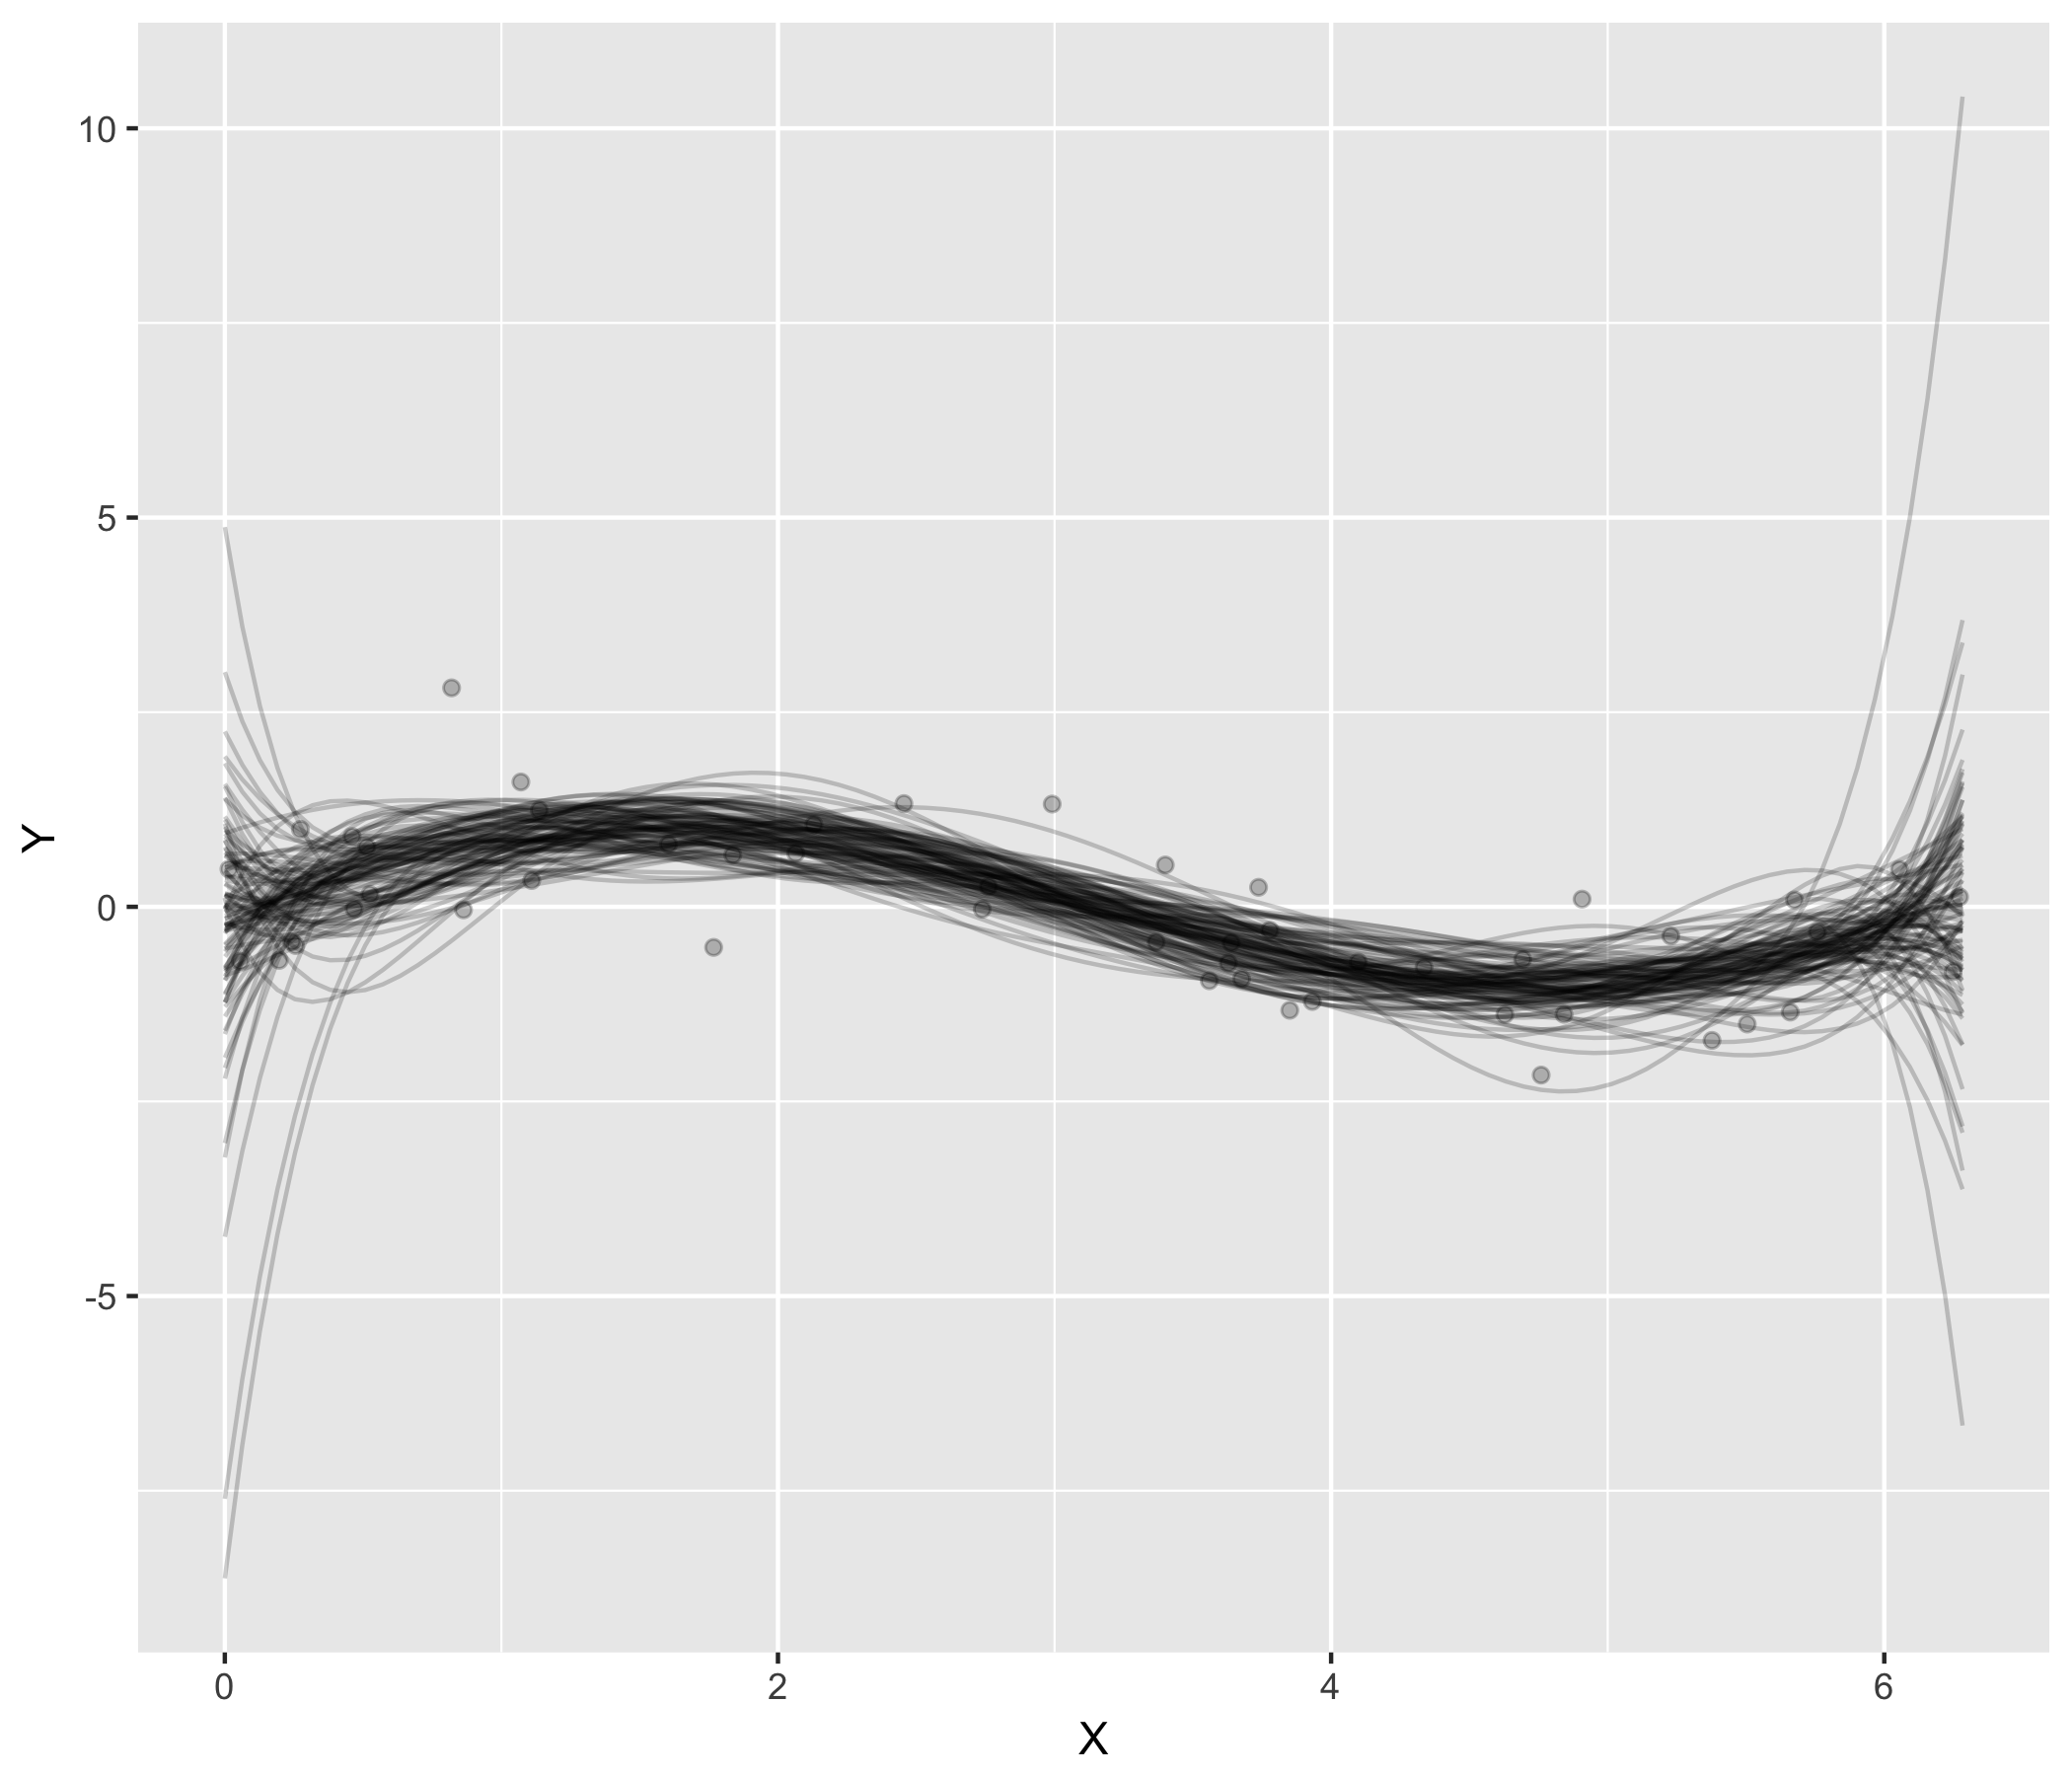
\includegraphics[scale=0.08]{model_variance_septic}
  \end{figure}
\end{frame}
%
%
\begin{frame}
  Increasing the complexity of the model can result in lower bias, and hence a
  lower asymptotic error rate, but enough data is needed to overcome the
  additional model variance:
  \begin{figure}
    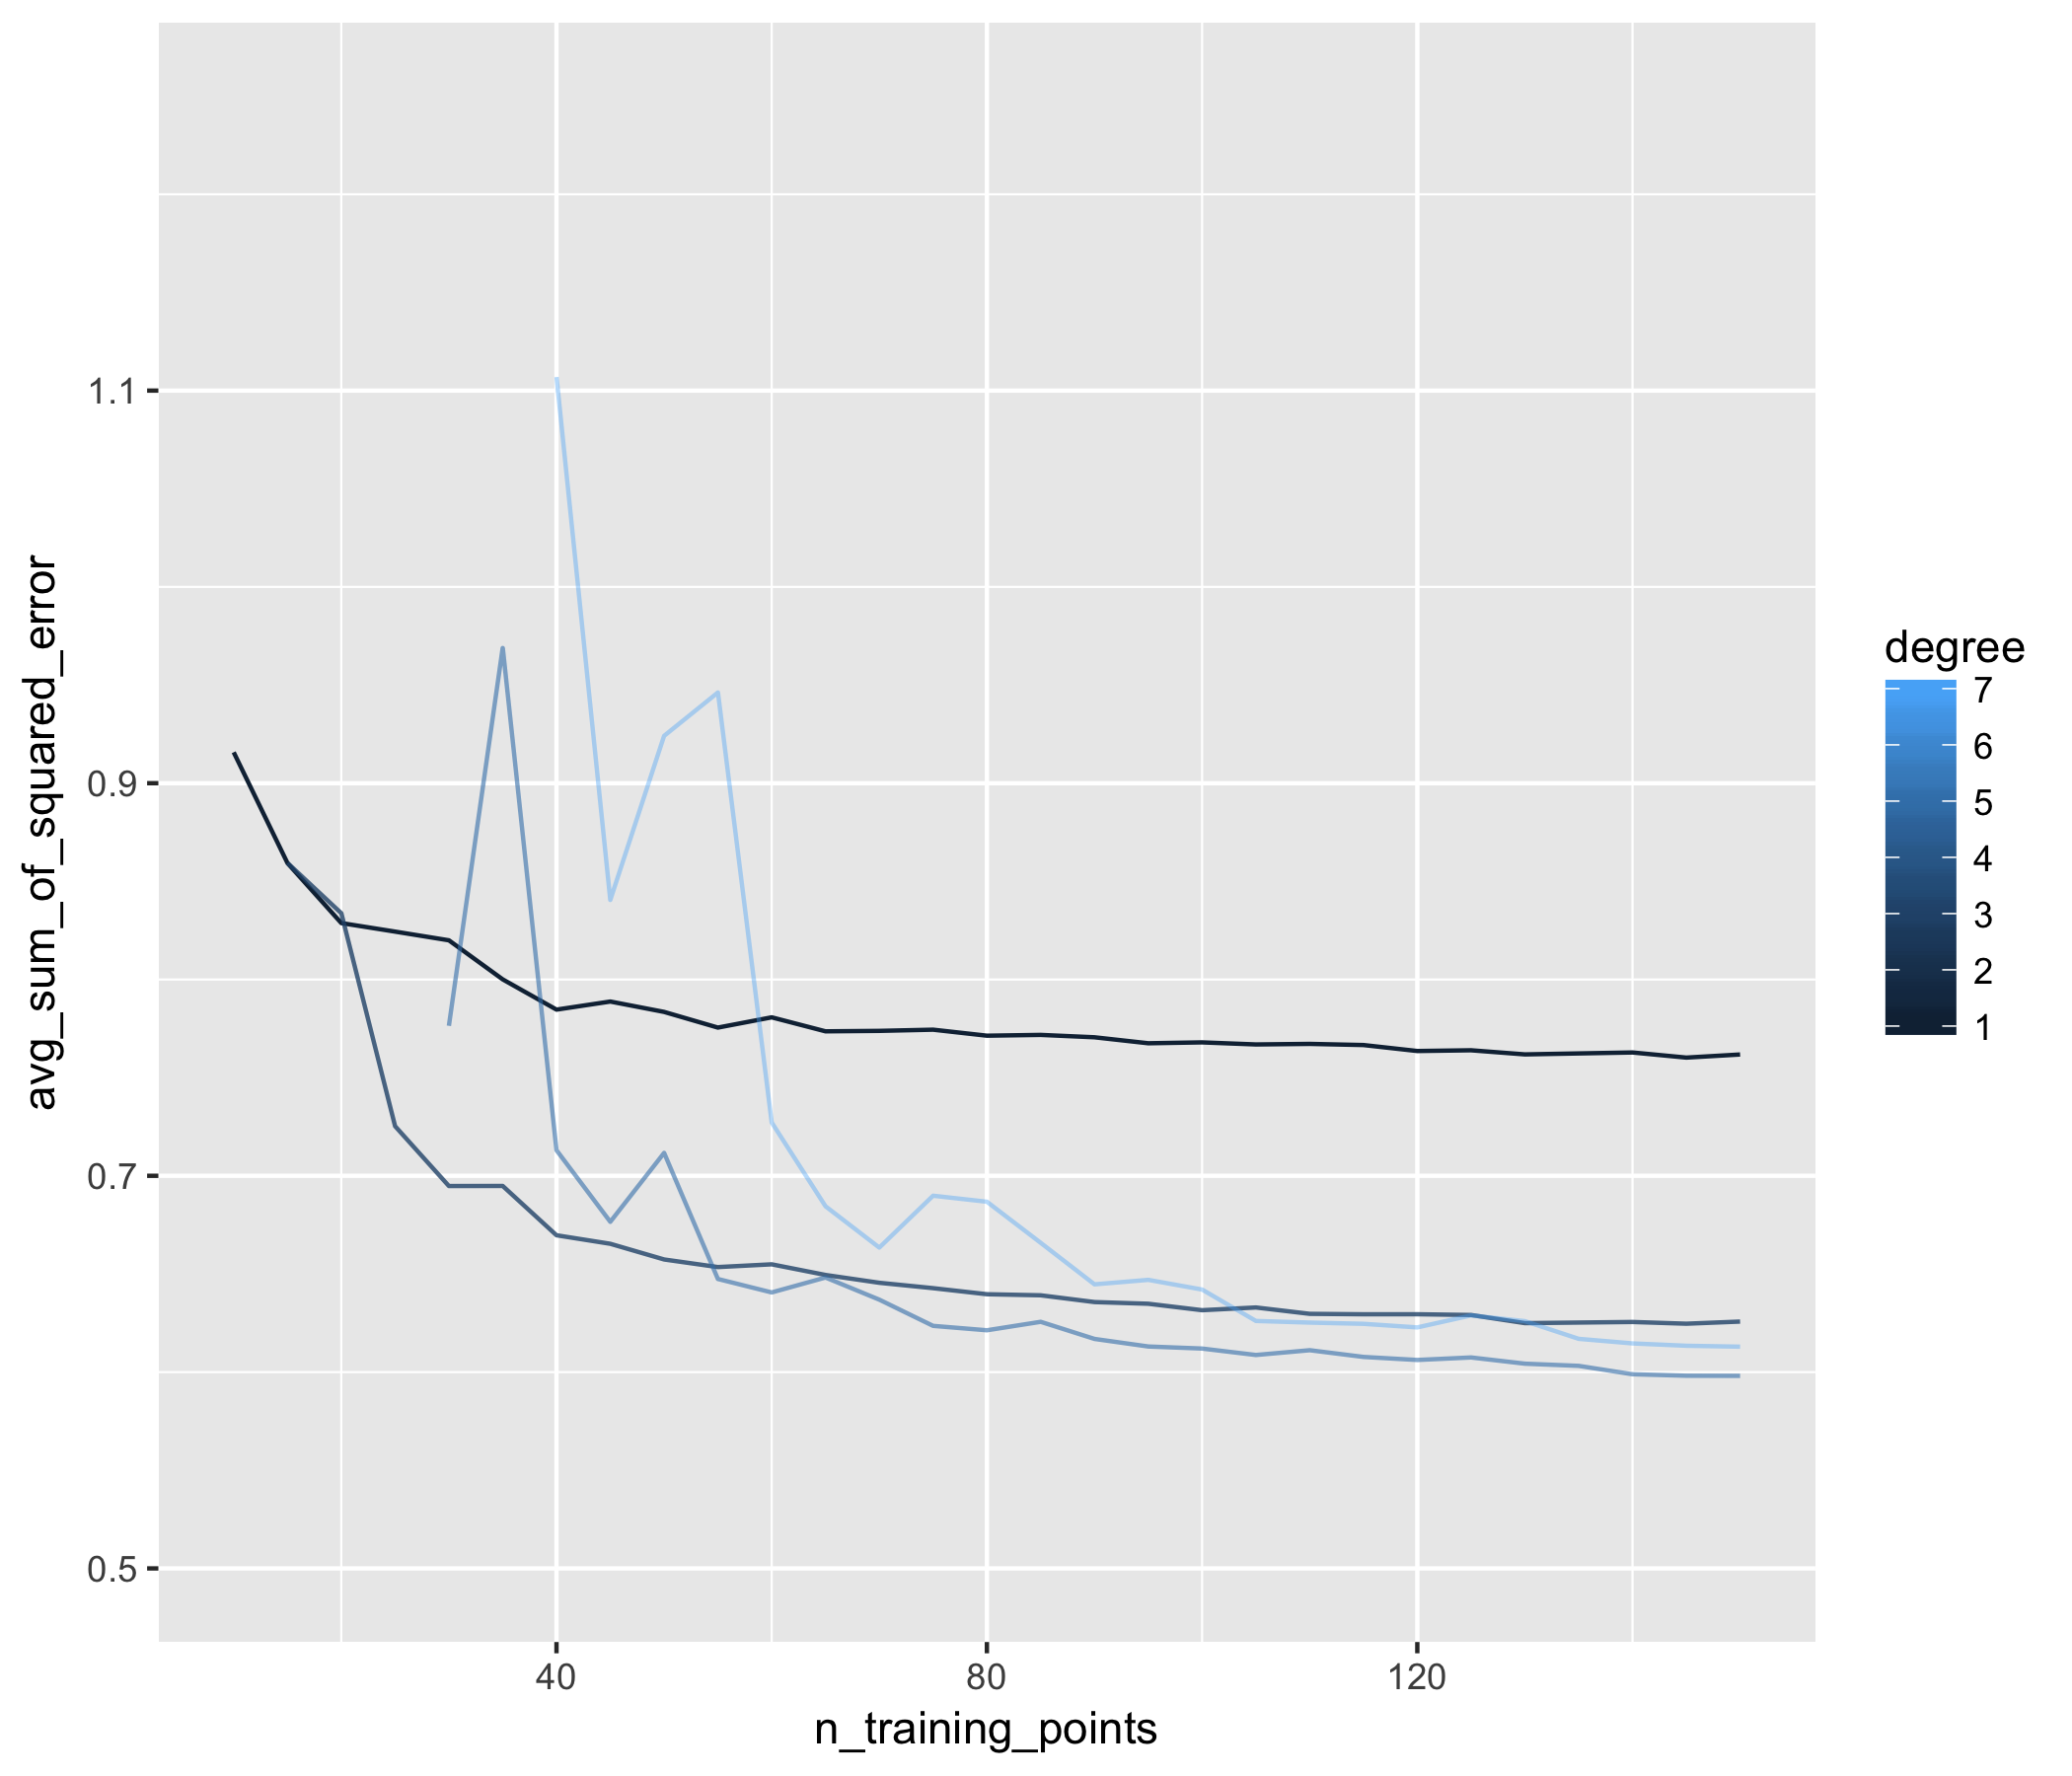
\includegraphics[scale=0.09]{out_of_sample_learning_curves}
  \end{figure}
\end{frame}
%
%
\begin{frame}
  If the complexity is increased too much, the variance can dominate, causing
  the expected error rate to increase
  \begin{figure}
    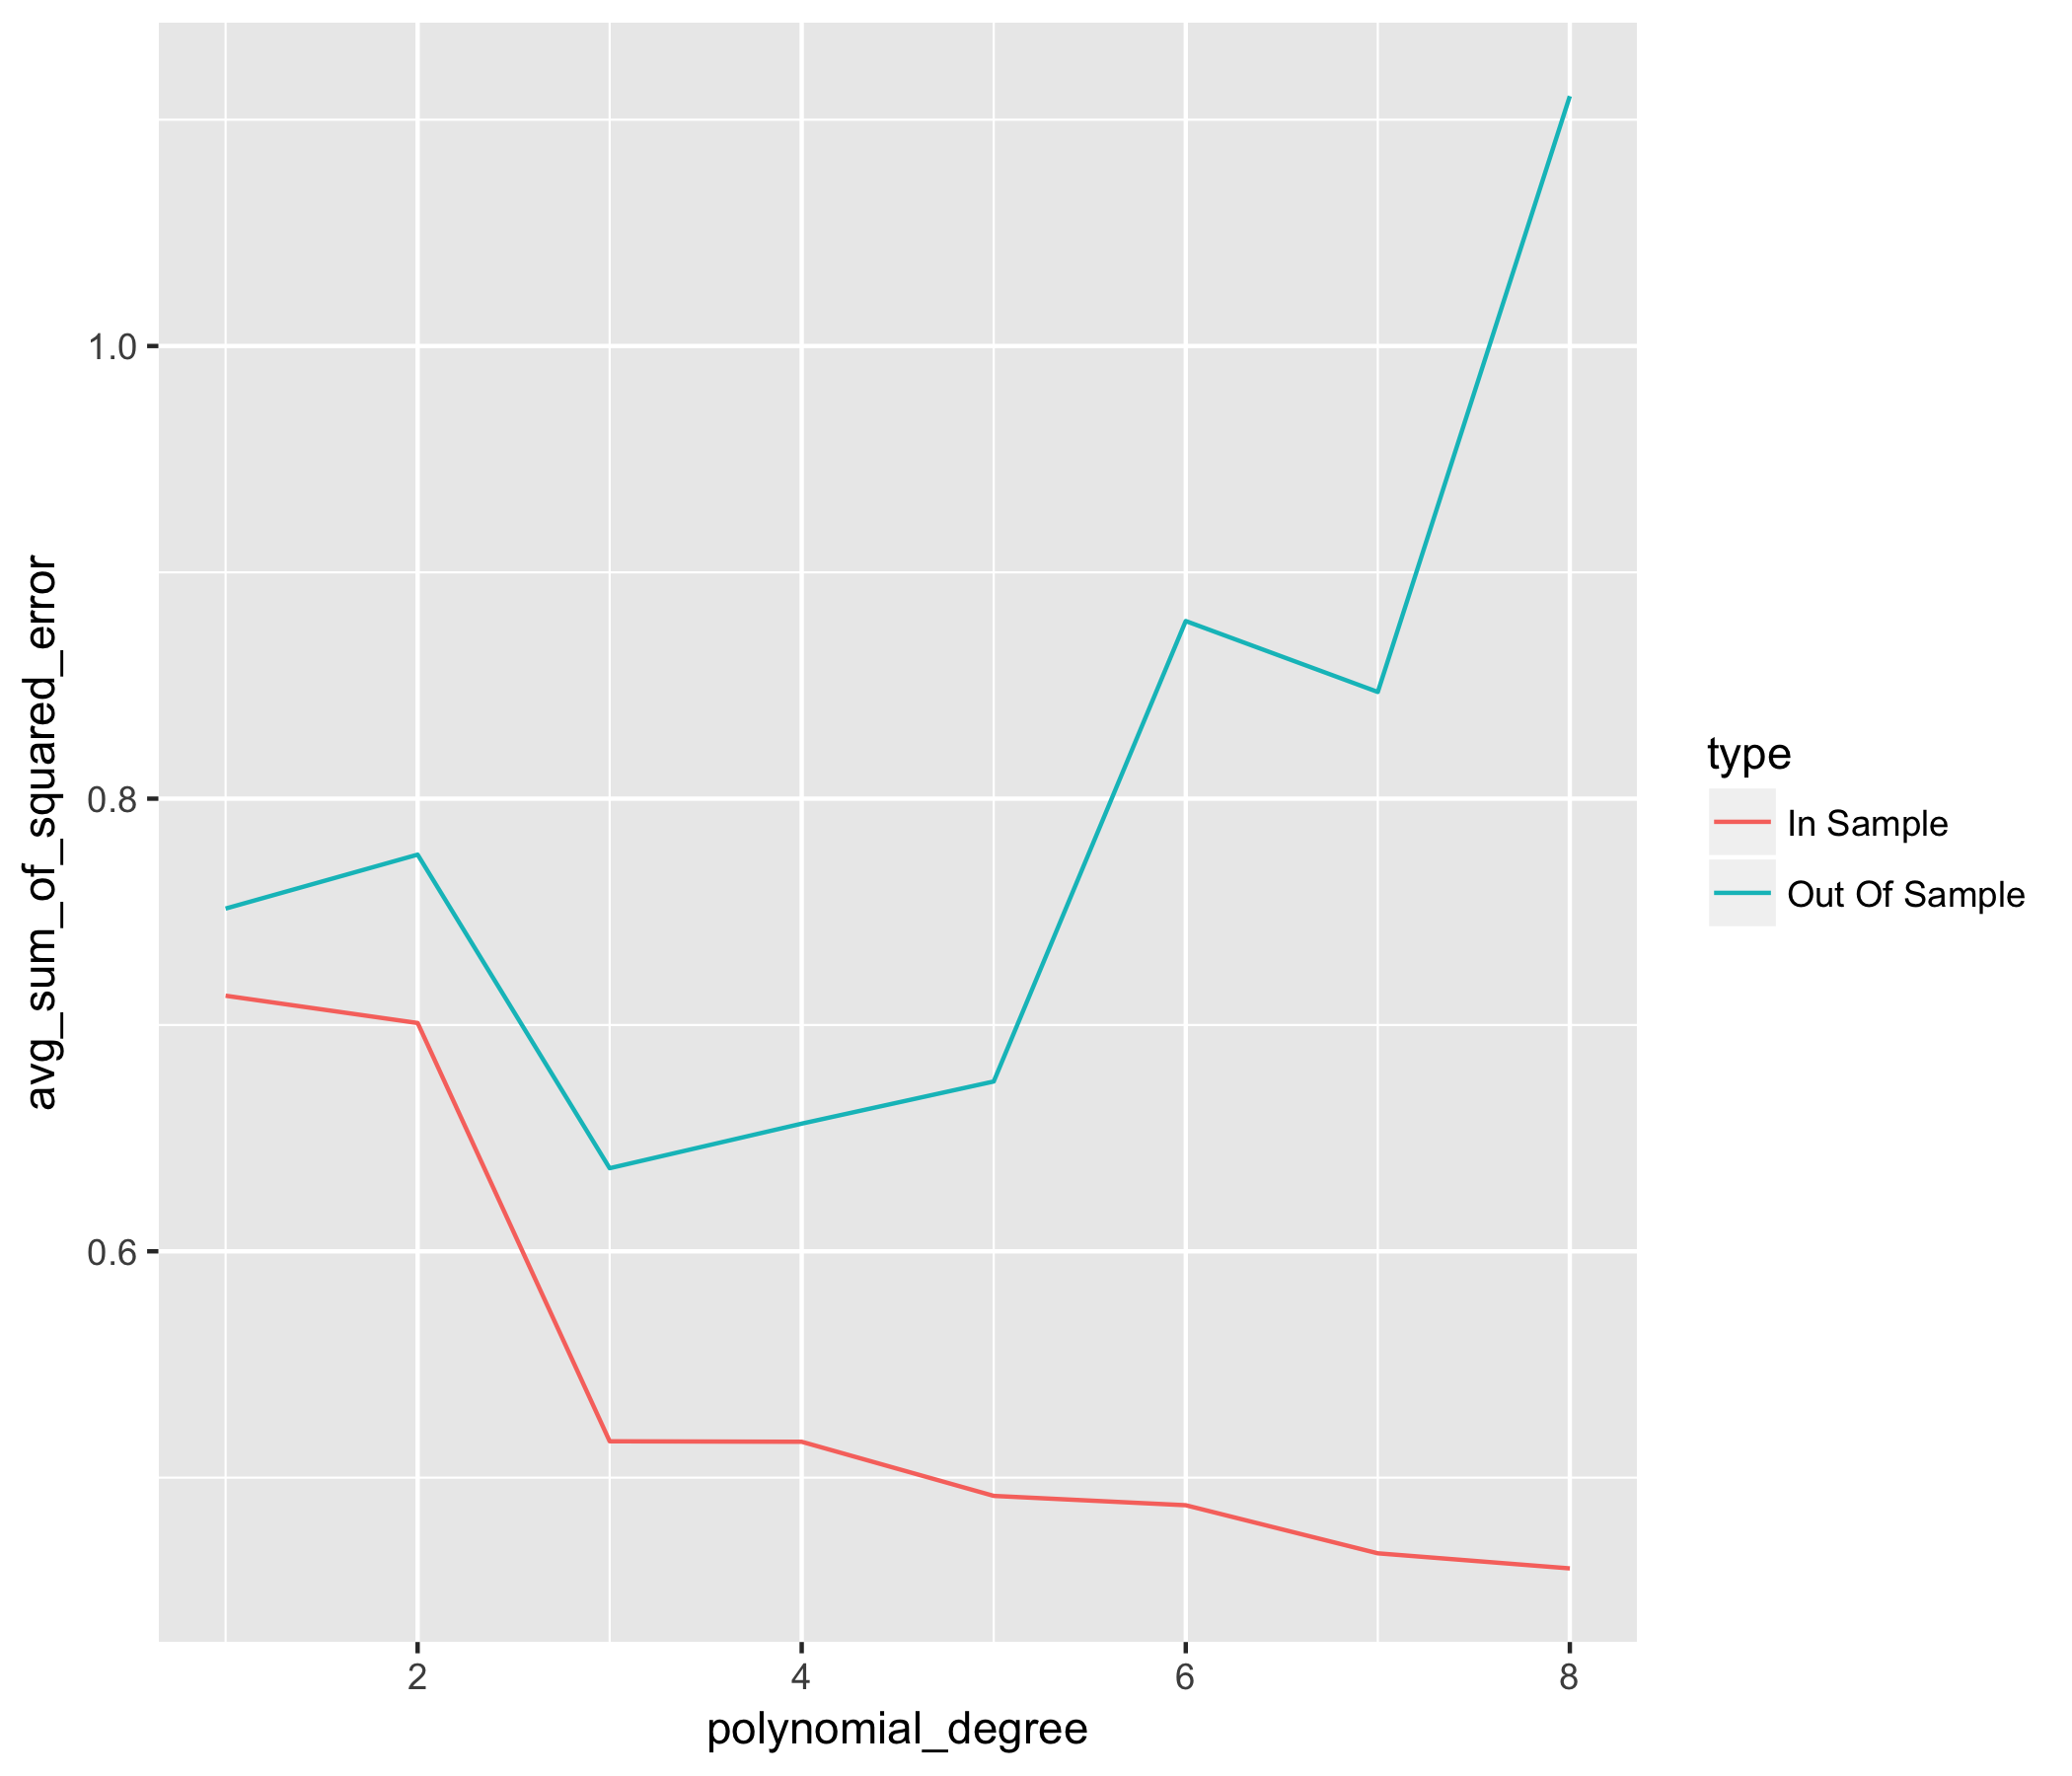
\includegraphics[scale=0.09]{learning_curves_by_degree}
  \end{figure}
\end{frame}
%
%
\begin{frame}
  Finally, increasing the irreducible error rate also increases the model variance:
  \begin{figure}
    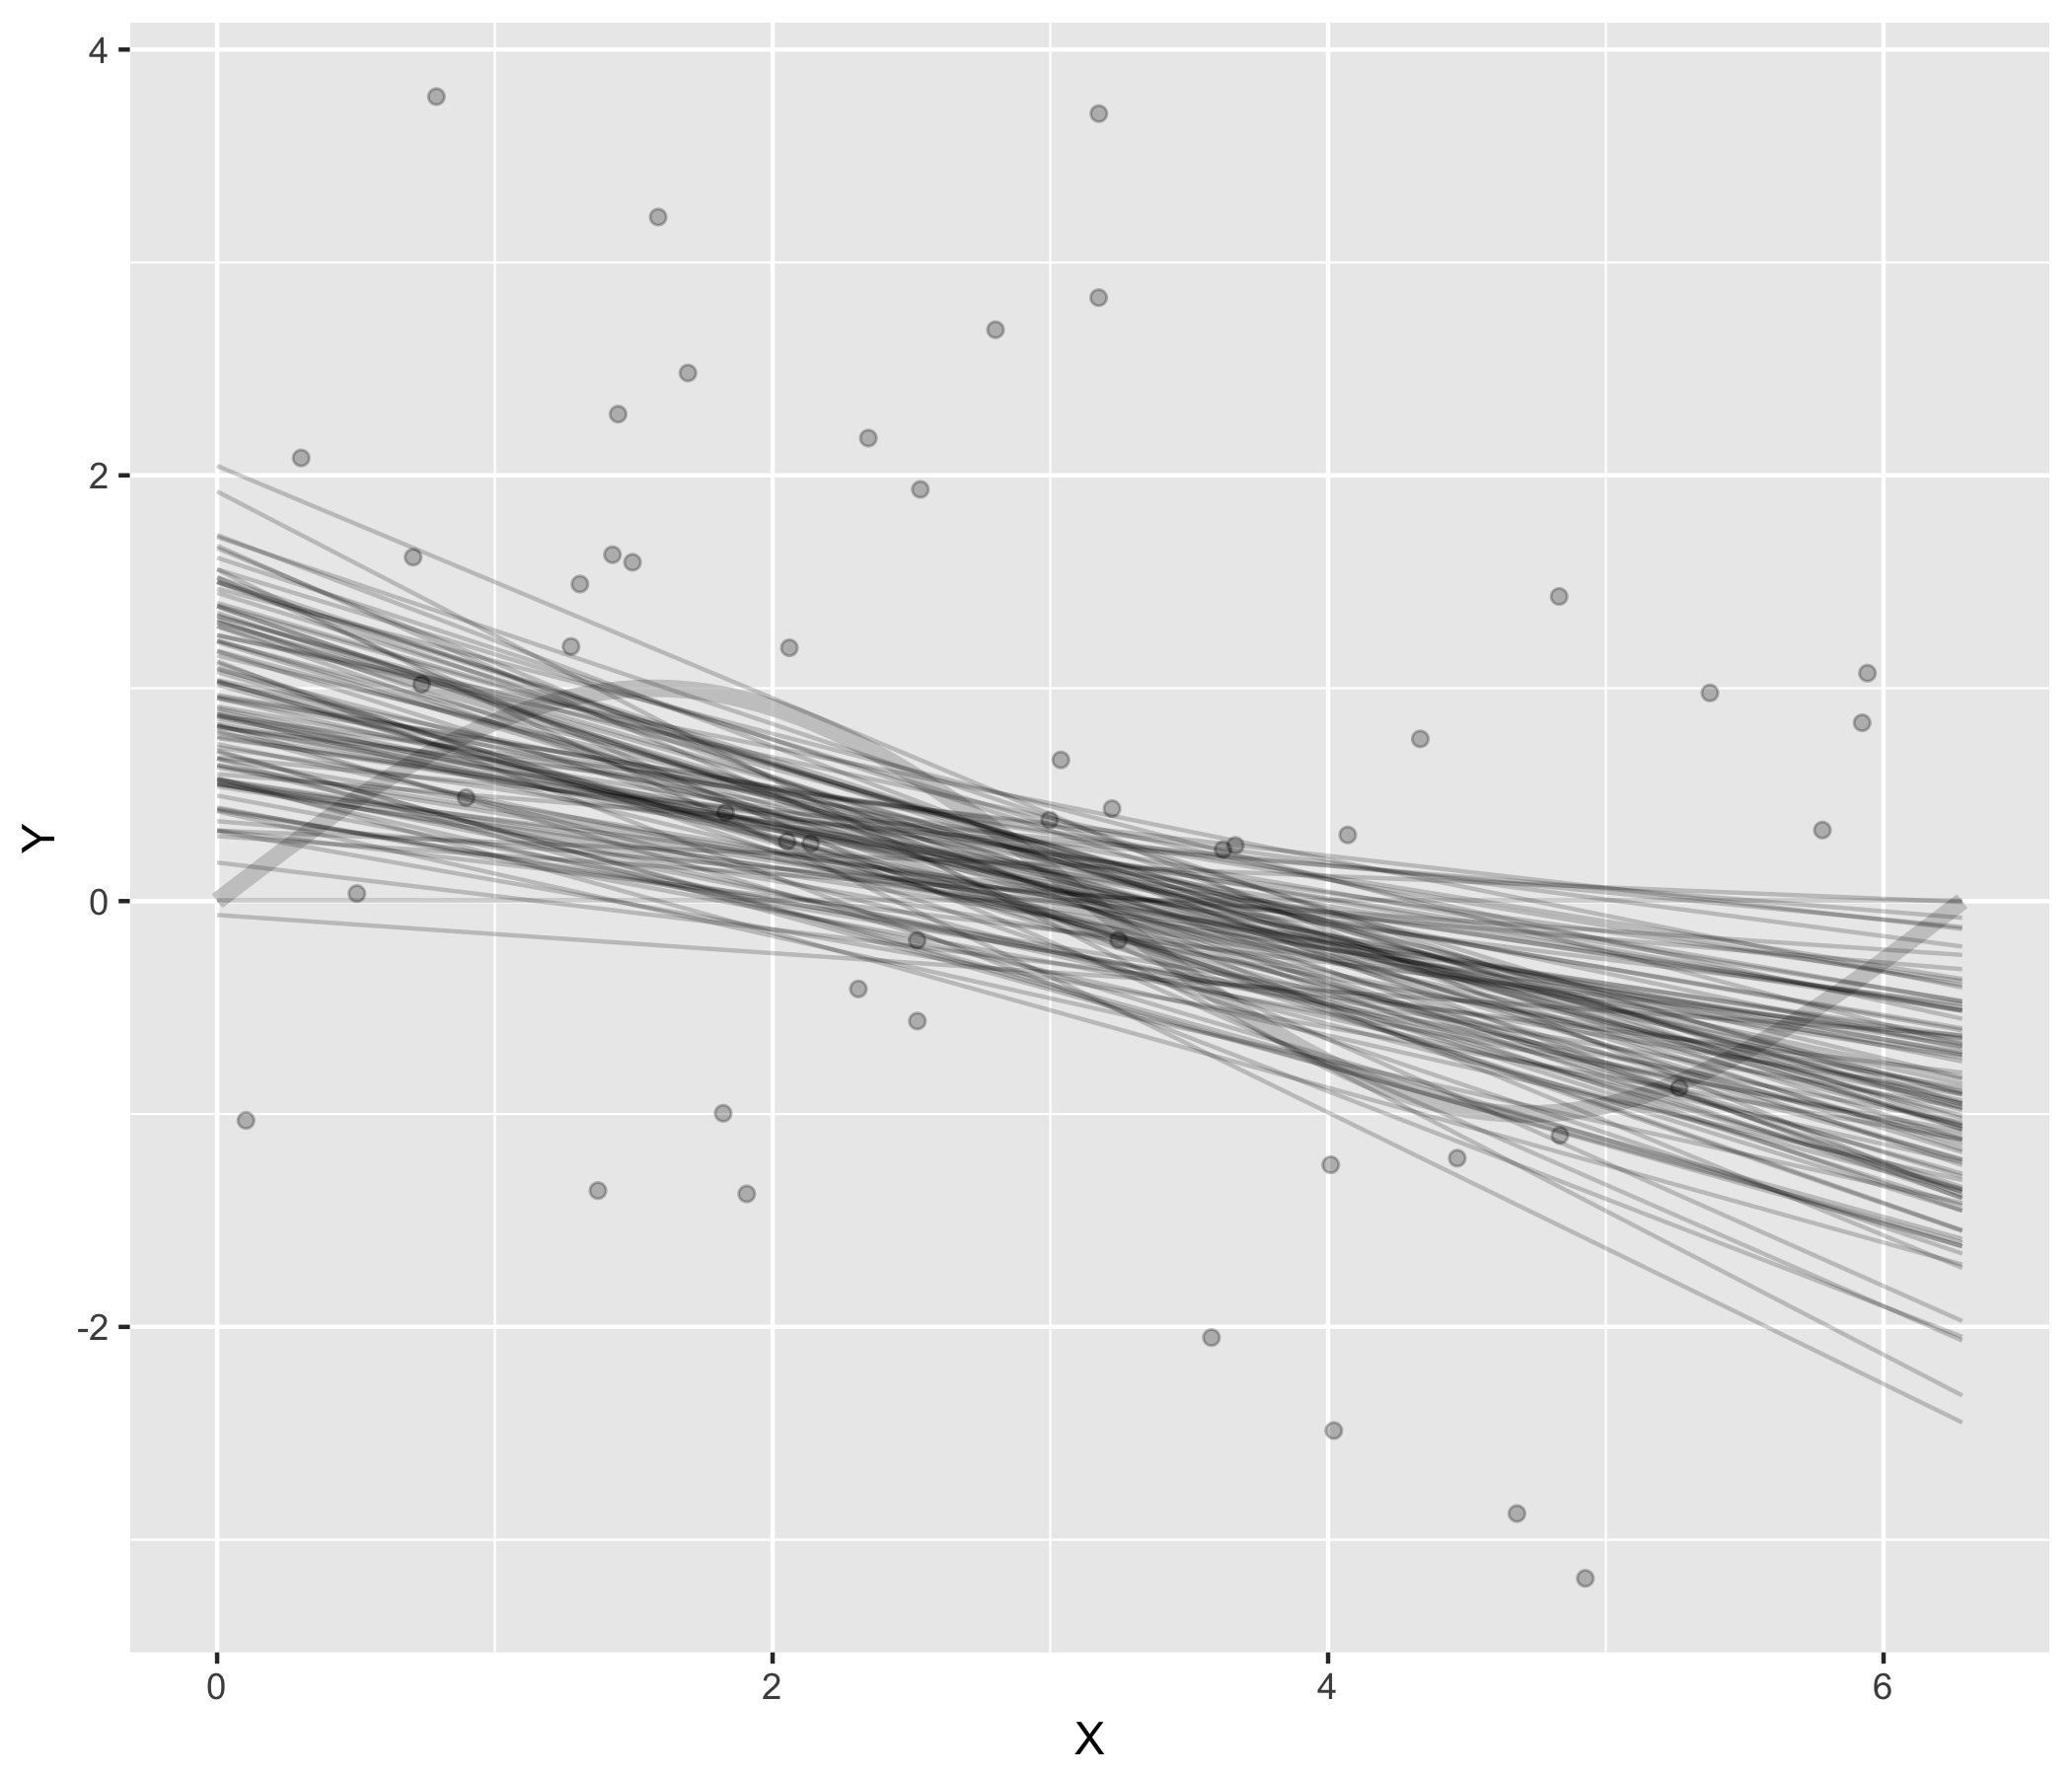
\includegraphics[scale=0.09]{model_variance_more_error}
  \end{figure}
\end{frame}
%
%
\begin{frame}
  A point derived from this discussion is especially important.  The complexity
  of a model should be a function of the \textbf{quantity} and \textbf{quality}
  of the data available.
  \begin{itemize}
    \item \textbf{Quantity}: The variance is a function of the number of samples
    available to train.
    \item \textbf{Quality}: The variance is a function of the irreducible error rate.
  \end{itemize}
\end{frame}
%
%gt
\begin{frame}
  The complexity of a model specification should \textbf{not} be based on
  supposed apriori knowledge of the complexity of the signal function, as
  seductive as this impulse is.
\end{frame}
%
%
\begin{frame}
  This is demonstrated here:
  \begin{figure}
    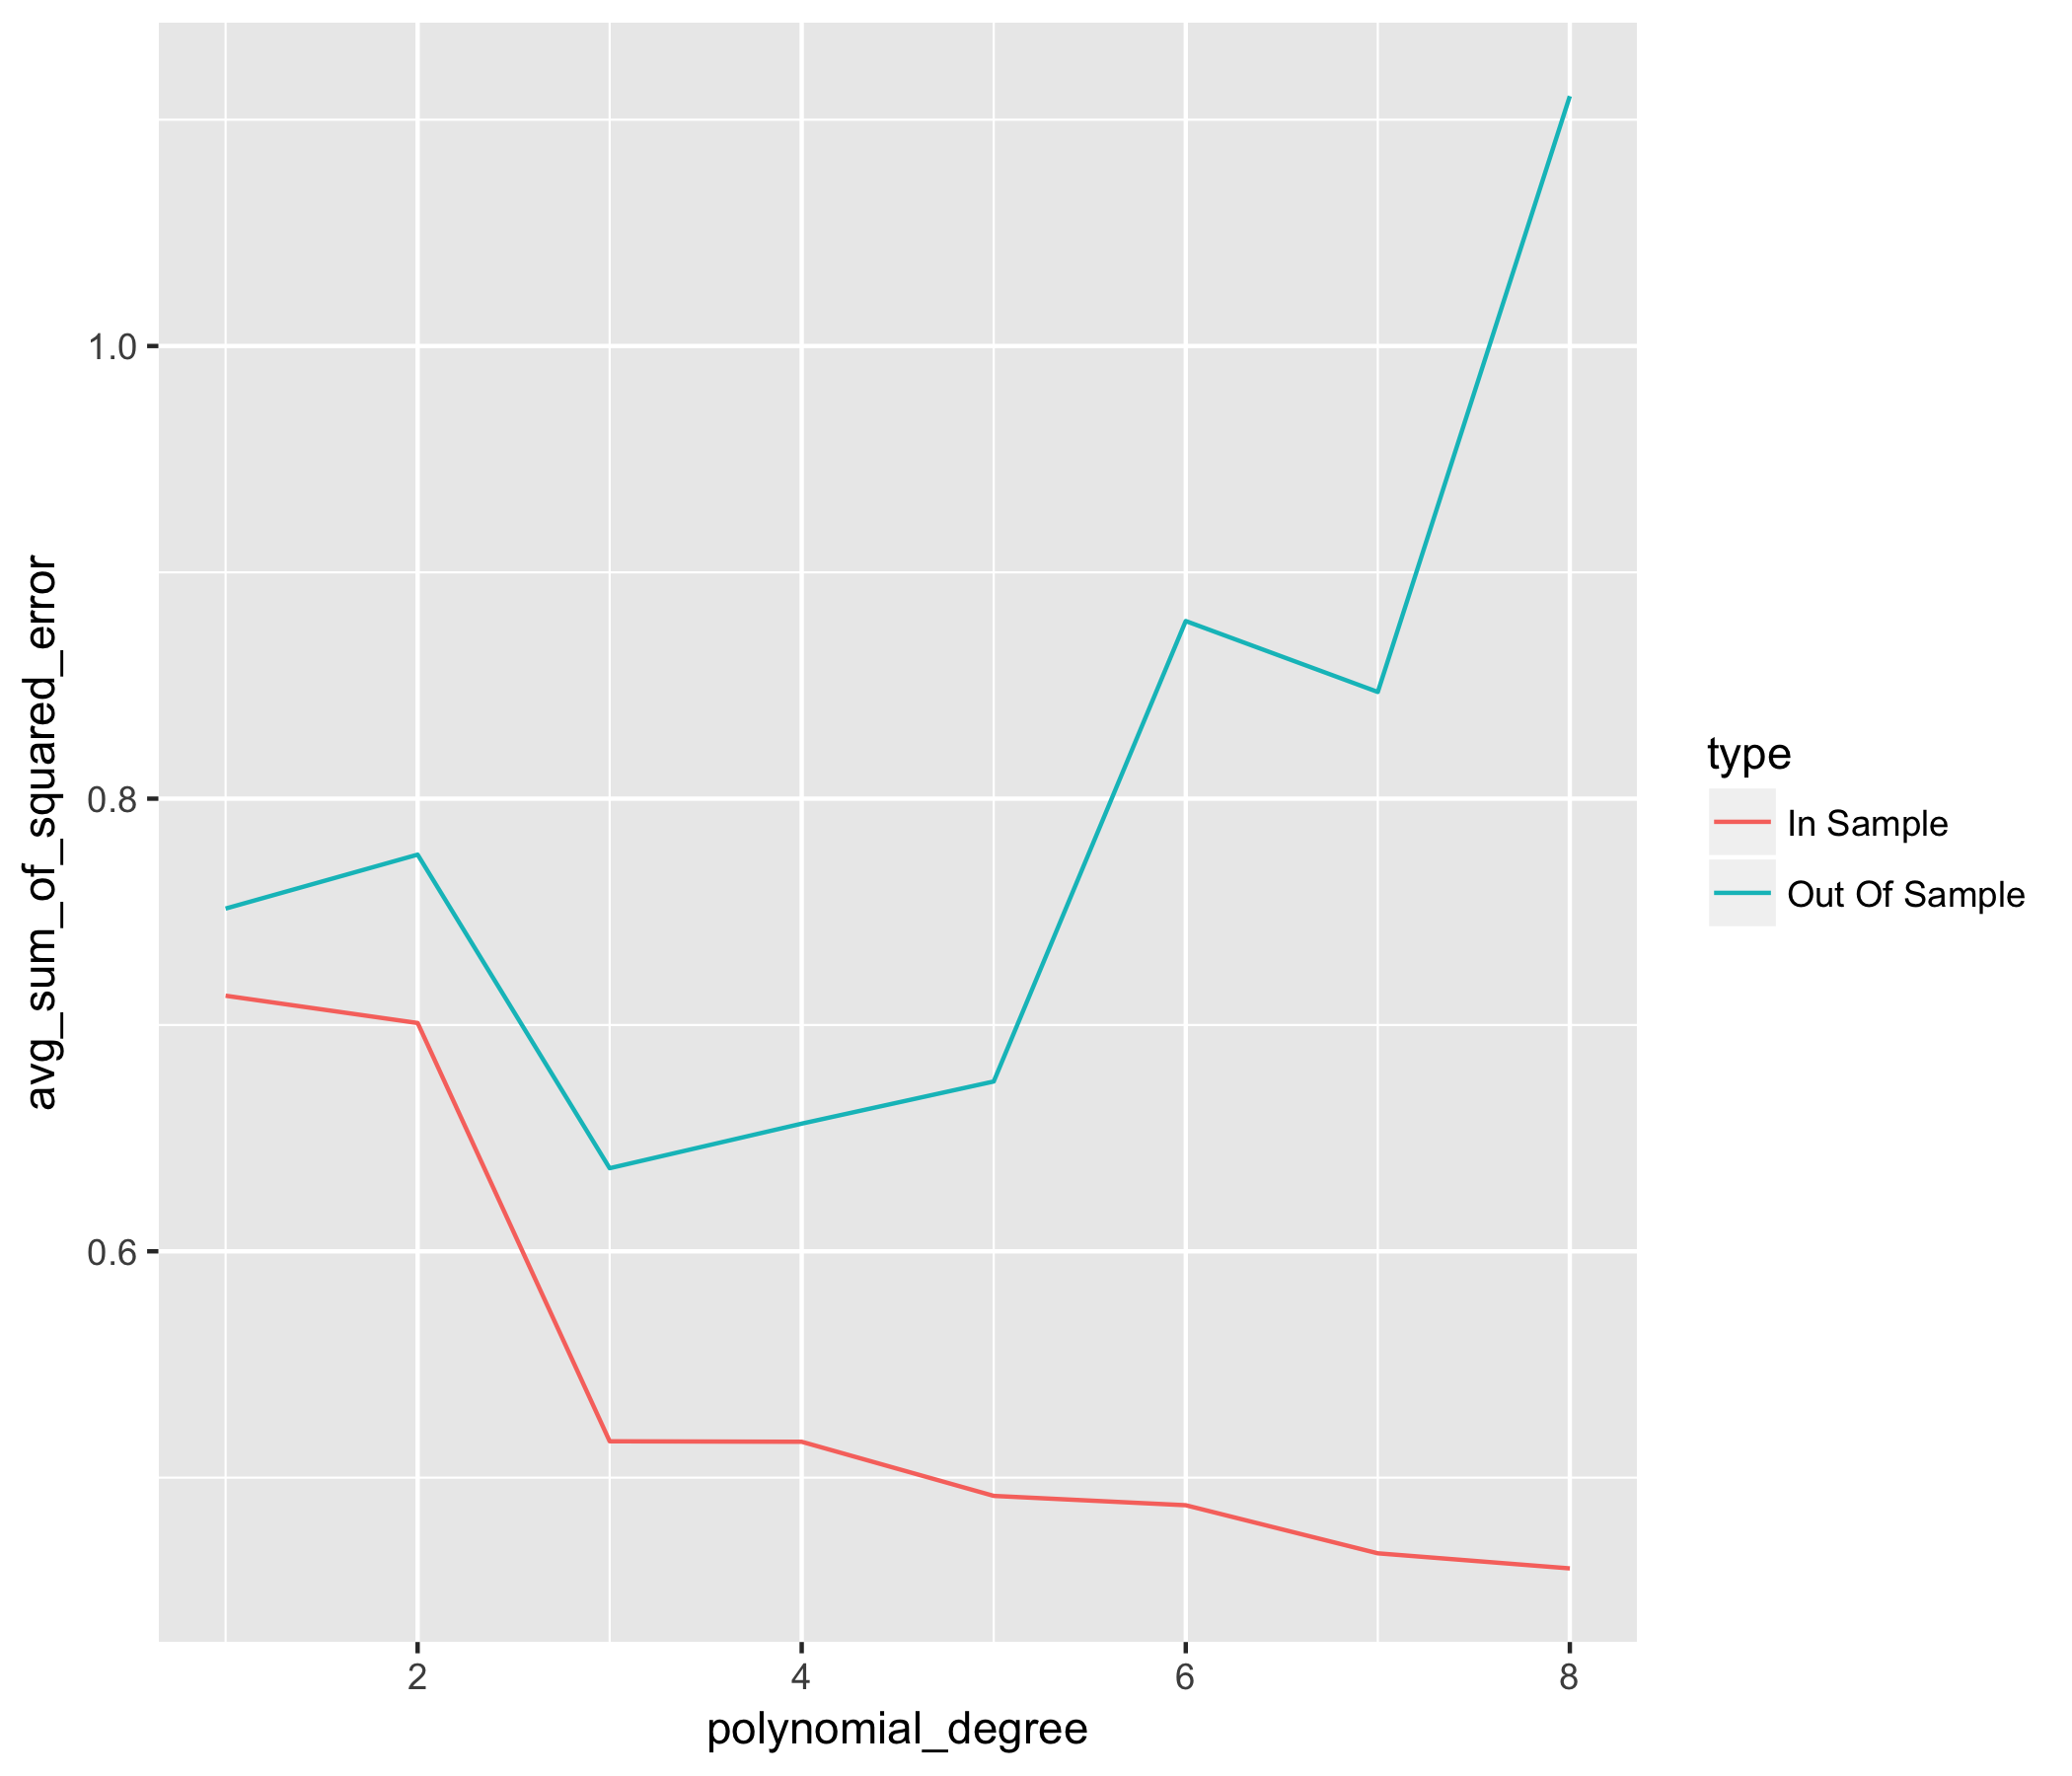
\includegraphics[scale=0.09]{learning_curves_by_degree}
  \end{figure}
  No polynomial curve can capture the true signal completely, but an ideal fit
  is closer the higher the degree.  None-the-less, the decrease in bias is
  overcome by the increase in variance.
\end{frame}

